%%%%%%%%%%%%%%%%%%%%%%%%%%%%%%%%%%%%%%%%%
% Masters/Doctoral Thesis 
% LaTeX Template
% Version 2.4 (22/11/16)
%
% This template has been downloaded from:
% http://www.LaTeXTemplates.com
%
% Version 2.x major modifications by:
% Vel (vel@latextemplates.com)
%
% This template is based on a template by:
% Steve Gunn (http://users.ecs.soton.ac.uk/srg/softwaretools/document/templates/)
% Sunil Patel (http://www.sunilpatel.co.uk/thesis-template/)
%
% Template license:
% CC BY-NC-SA 3.0 (http://creativecommons.org/licenses/by-nc-sa/3.0/)
%
%%%%%%%%%%%%%%%%%%%%%%%%%%%%%%%%%%%%%%%%%

%----------------------------------------------------------------------------------------
%	PACKAGES AND OTHER DOCUMENT CONFIGURATIONS
%----------------------------------------------------------------------------------------

\documentclass[
11pt, % The default document font size, options: 10pt, 11pt, 12pt
oneside, % Two side (alternating margins) for binding by default, uncomment to switch to one side
english, % ngerman for German
onehalfspacing, % Single line spacing, alternatives: onehalfspacing or doublespacing
%draft, % Uncomment to enable draft mode (no pictures, no links, overfull hboxes indicated)
%nolistspacing, % If the document is onehalfspacing or doublespacing, uncomment this to set spacing in lists to single
%liststotoc, % Uncomment to add the list of figures/tables/etc to the table of contents
%toctotoc, % Uncomment to add the main table of contents to the table of contents
%parskip, % Uncomment to add space between paragraphs
%nohyperref, % Uncomment to not load the hyperref package
headsepline, % Uncomment to get a line under the header
chapterinoneline, % Uncomment to place the chapter title next to the number on one line
%consistentlayout, % Uncomment to change the layout of the declaration, abstract and acknowledgements pages to match the default layout
]{MastersDoctoralThesis} % The class file specifying the document structure

\usepackage[utf8]{inputenc} % Required for inputting international characters
\usepackage[T1]{fontenc} % Output font encoding for international characters
\let\latinencoding\relax
\usepackage{fontspec} % Better font handling

\usepackage[newfloat]{minted} % Code Highlighting
\usepackage{caption}
\usepackage{tcolorbox}
\usepackage{etoolbox}

\newenvironment{code}{\captionsetup{type=listing}}{}
\SetupFloatingEnvironment{listing}{name=Snippet}

\BeforeBeginEnvironment{minted}{\begin{tcolorbox}}%
\AfterEndEnvironment{minted}{\end{tcolorbox}}%


\setmainfont{Palatino Linotype}
\setmonofont[Scale=0.85]{Consolas}

\usepackage[backend=bibtex,style=numeric,natbib=true]{biblatex} % Use the bibtex backend with the authoryear citation style (which resembles APA)

\addbibresource{bibliography.bib} % The filename of the bibliography

\usepackage[autostyle=true]{csquotes} % Required to generate language-dependent quotes in the bibliography

\newcommand*\justify{%
    \fontdimen2\font=0.4em% interword space
    \fontdimen3\font=0.2em% interword stretch
    \fontdimen4\font=0.1em% interword shrink
    \fontdimen7\font=0.1em% extra space
    \hyphenchar\font=`\-% allowing hyphenation
}


%----------------------------------------------------------------------------------------
%	MARGIN SETTINGS
%----------------------------------------------------------------------------------------

\geometry{
	paper=letterpaper, % Change to letterpaper for US letter
	inner=2.5cm, % Inner margin
	outer=3.8cm, % Outer margin
	bindingoffset=.5cm, % Binding offset
	top=3.5cm, % Top margin
	bottom=3cm, % Bottom margin
	%showframe, % Uncomment to show how the type block is set on the page
}

%----------------------------------------------------------------------------------------
%	THESIS INFORMATION
%----------------------------------------------------------------------------------------

\thesistitle{A Big Data Architecture: from Ingestion to Analytics} % Your thesis title, this is used in the title and abstract, print it elsewhere with \ttitle
\supervisor{Dott. Luca \textsc{Oneto}} % Your supervisor's name, this is used in the title page, print it elsewhere with \supname
\examiner{} % Your examiner's name, this is not currently used anywhere in the template, print it elsewhere with \examname
\degree{Corso di Laurea Magistrale in Ingegneria Informatica} % Your degree name, this is used in the title page and abstract, print it elsewhere with \degreename
\author{Federico \textsc{D'Ambrosio}, Edoardo \textsc{Ferrante}} % Your name, this is used in the title page and abstract, print it elsewhere with \authorname
\addresses{} % Your address, this is not currently used anywhere in the template, print it elsewhere with \addressname

\subject{Data Analysis} % Your subject area, this is not currently used anywhere in the template, print it elsewhere with \subjectname
\keywords{} % Keywords for your thesis, this is not currently used anywhere in the template, print it elsewhere with \keywordnames
\university{{Università degli studi di Genova}} % Your university's name and URL, this is used in the title page and abstract, print it elsewhere with \univname
\department{\href{http://www.dibris.unige.it/}{DIBRIS - Department of Informatics, Bioengineering, Robotics and Systems Engineering}} % Your department's name and URL, this is used in the title page and abstract, print it elsewhere with \deptname
\group{\href{http://researchgroup.university.com}{Research Group Name}} % Your research group's name and URL, this is used in the title page, print it elsewhere with \groupname
\faculty{\href{http://www.informatica.ingegneria.unige.it/}{Ingegneria Informatica}} % Your faculty's name and URL, this is used in the title page and abstract, print it elsewhere with \facname

\AtBeginDocument{
\hypersetup{pdftitle=\ttitle} % Set the PDF's title to your title
\hypersetup{pdfauthor=\authorname} % Set the PDF's author to your name
\hypersetup{pdfkeywords=\keywordnames} % Set the PDF's keywords to your keywords
}

\begin{document}
\hypersetup{colorlinks, urlcolor=blue, linkcolor=blue}

\frontmatter % Use roman page numbering style (i, ii, iii, iv...) for the pre-content pages

\pagestyle{plain} % Default to the plain heading style until the thesis style is called for the body content

%----------------------------------------------------------------------------------------
%	TITLE PAGE
%----------------------------------------------------------------------------------------

\begin{titlepage}
%\linespread{1.5}
\thispagestyle{empty}
\begin{center}
	
\includegraphics[width=0.2\linewidth]{Figures/unige.eps}
\end{center}

\begin{center}
	\LARGE\sc
	\univname\\
	
	\vspace{0.5cm}
	\large
	\degreename\\
\end{center}

\begin{center}
	\small
	Tesi di Laurea per il conseguimento del titolo di\\
	Dottore Magistrale in Ingegneria Informatica\\
\end{center}

\vfill

\begin{center} 
	\LARGE
	{\bf \ttitle}\\
	\vspace{0.5cm}
	\large
	\authorname\\
	\vspace{0.5cm}
	\small
	Anno Accademico 2016/2017
\end{center}

\vfill

\begin{tabular}{lll}%
	{\em Relatore}:	& Luca Oneto\\
	{\em Relatore}:	& Davide Anguita\\
    {\em Correlatore}: & Alberto Galletto\\
\end{tabular} 

\hfill


\end{titlepage}


%----------------------------------------------------------------------------------------
%	QUOTATION PAGE
%----------------------------------------------------------------------------------------

%\vspace*{0.2\textheight}

%\noindent\enquote{\itshape Thanks to my solid academic training, today I can write hundreds of words on virtually any topic without possessing a shred of information, which is how I got a good job in journalism.}\bigbreak

%\hfill Dave Barry

%----------------------------------------------------------------------------------------
%	ABSTRACT PAGE
%----------------------------------------------------------------------------------------

\begin{abstract}
\addchaptertocentry{\abstractname} % Add the abstract to the table of contents
This thesis aims to analyse the many components required for a Big Data infrastructure and to identify the ideal ones among the state-of-the-art products in the ever renewing environment of Big Data analytics, amidst the context of Business Intelligence and Data Driven Decision Making for industries.
Real world applications need, in this context, a well defined, scalable and flexible infrastructure with interchangeable components as the use case needs. In order to show this, we applied the aforementioned concepts in an air traffic monitoring application, a service similar to those provided by FlightRadar24 or FlightAware, through the implementation of a data processing pipeline, starting from the ingestion of the raw data, ending with the processing and visualization of analytics.
The results show that the tools available are powerful and customizable and allow for a wide range of useful implementations ranging from reporting systems and real time monitoring to decision support applications.
\end{abstract}

%----------------------------------------------------------------------------------------
%	ACKNOWLEDGEMENTS
%----------------------------------------------------------------------------------------

%\begin{acknowledgements}
%\addchaptertocentry{\acknowledgementname} % Add the acknowledgements to the table of contents
%The acknowledgments and the people to thank go here, don't forget to include your project advisor\ldots
%\end{acknowledgements}

%----------------------------------------------------------------------------------------
%	LIST OF CONTENTS/FIGURES/TABLES PAGES
%----------------------------------------------------------------------------------------

\tableofcontents % Prints the main table of contents


%----------------------------------------------------------------------------------------
%	DEDICATION
%----------------------------------------------------------------------------------------

%\dedicatory{For/Dedicated to/To my\ldots} 

%----------------------------------------------------------------------------------------
%	THESIS CONTENT - CHAPTERS
%----------------------------------------------------------------------------------------

\mainmatter % Begin numeric (1,2,3...) page numbering

\pagestyle{thesis} % Return the page headers back to the "thesis" style

% Include the chapters of the thesis as separate files from the Chapters folder
% Uncomment the lines as you write the chapters


\chapter{Introduction}

\section{Big Data: What are they?}

Big Data, as the name suggests, are a collection of huge amount of data, that requires a sophisticated infrastructure to be managed and for its valuable information to be extracted.\newline
It is customary to define Big Data as having three fundamental features, known as the \textbf{3 Vs}:

\paragraph{Volume}

The quantity of data generated and stored must be huge, even in the orders of magnitude of the Brontobytes ($10^{27}$ bytes).
Every bit of data might hide some interesting piece of information, so the infrastructure must always be able to retrieve as much data as possible and store it for later use.

\paragraph{Velocity}

In the ever changing environment of our digital world, floating in a widespread network linking every device of our life (Internet of Things), data are flowing at an increasing pace. The infrastructure must be able to keep up with this rhythm, as data ages faster each day.

\paragraph{Variety}

With the rapid increase of published information, known as information explosion, data has begun to diversify more and more, and it is now unrealistic to expect just structured textual information such as classical database tables; the new data flow includes unstructured data such as images, audio, PDFs and raw text files. The infrastructure must be able to extract information from heterogeneous sources.


\section{A Big Data Infrastructure}

As we have established, a Big Data Infrastructure must meet several requirements in order to function properly. 
To manage the complexity needed for this heavy feat, the whole system is organized in several layers; each layer may be implemented with one of several products without changing the rest of the structure.

\begin{figure}
	\centering
	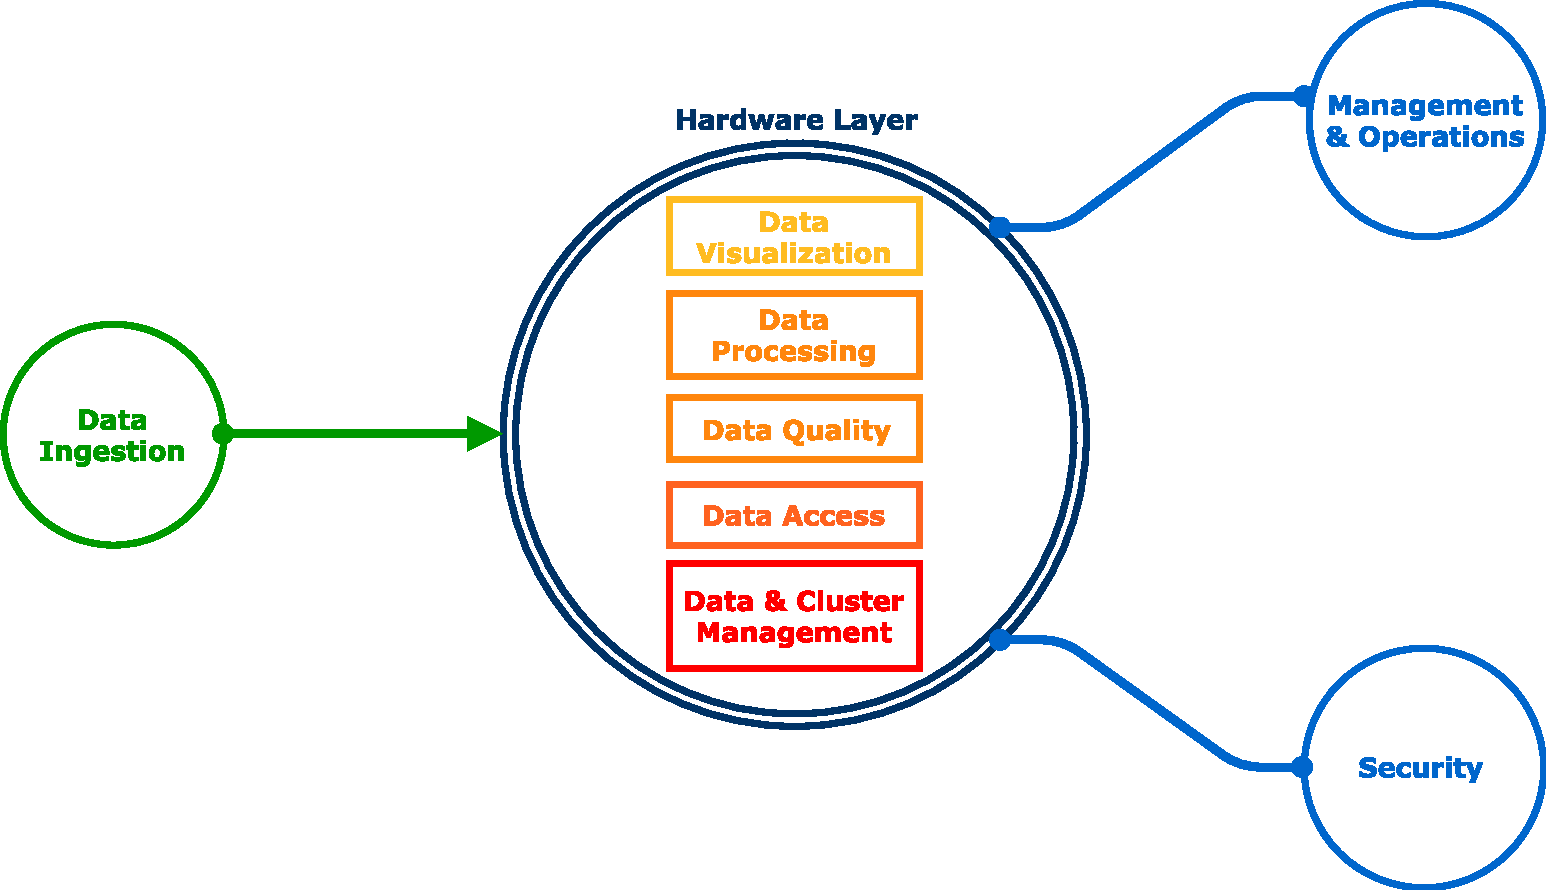
\includegraphics[scale=0.6]{Figures/stack_infrastructure}
	\decoRule
	\caption[Infrastructural Stack]{A model of a Big Data Infrastructure}
	\label{fig:InfrastructuralStack}
\end{figure}

\paragraph{Hardware}

At the foundations of the stack we find the hardware (real or virtualised), which is, in general, a group of several machines called a cluster.\newline
The machines are tied together in a single network each to one another, so that communication between them is as easy and reliable as possible and the cluster can act like a single machine with high performance and reliability.

\paragraph{Data \& Cluster Management}

Over the first layer of software provided by each machine's Operating System, the cluster needs an interface, so that from an higher point of view, like that of a developer or of an application, the whole system may seem a single entity. \newline
That interface, provided by the Data \& Cluster Management layer, must offer: 
\begin{itemize}
	\item A distributed filesystem, able to be accessed like a standard one while providing high fault tolerance thanks to the replication of data on the different machines of the cluster.
	\item A distributed Operating System, able to manage access to resources on the whole cluster and to schedule application jobs.
\end{itemize}

\paragraph{Data Access}

Having reached a more unified view on the cluster thanks to the previous layer, we can forget about the details of the single machines.\newline
As we would use databases on a normal computer, so we add, on top of the data access layer, a distributed database able to store our data efficiently and for easy access on the distributed filesystem.
Distributed databases come in different shapes and styles, ranging from the familiar relational ones to non-relational document stores and key-value row based stores.

\paragraph{Data Quality}

As mentioned before, our goals are to store as much data as we feasibly can and then process them: the acquisition of big data sets will often lead to a certain amount of dirty data and, what’s more, these huge swaths of data, even cleaned, could be hard to be accessed or made valuable because of their lack of a well defined structure.
\newline
Therefore, data must go through the Data Quality layer in order to be ready for further processing, this layer must offer applications for:
\begin{itemize}
	\item Data Cleaning, the process of detection, correction and removal of dirty data such as corrupt or wrong records or documents.
	\item Data Wrangling, the process of mapping raw data to a more structured format; wrangling unstructured data also helps their future Cleaning.
\end{itemize}

\paragraph{Data Processing}

Over all the previous strata, we can finally run some applications on the Data Processing layer; those applications, executed in jobs scheduled and managed by the distributed Operating System, process the clean data stored on the distributed database or on the distributed filesystem.\newline
This layer provides for distributed processing frameworks where applications can be deployed and run seamlessly on the cluster as a whole, in-memory or on disk, in batches or in real time.\newline
Processed data can then be stored again on the filesystem or on the database, formatted or enriched in information for later visualisation or further elaboration.

\paragraph{Data Visualisation}

The topmost layer of the main part of the stack is the Data Visualisation layer which supplies a visualising software, whose job is to load data stored on the database or filesystem, processed and enriched in the previous layer, and make its information intelligible to humans through the use of images, which can convey several dimensions on a 2D plot thanks to their geometric shape, position and size and their colours.

\paragraph{Data Ingestion}

Orbiting our main stack we find other transversal layers, first among them the Data Ingestion layer.\newline
As described, Big Data infrastructures must be able to handle huge amounts of incoming data at high speed and in real time; this layer provides for applications that can manage incoming real time traffic of data from a source to the cluster, through filtering, mediating and queueing. It might also involve real time cleaning, wrangling and processing applications.

\paragraph{Management \& Operations}

The complexity of the infrastructure with its numerous layers and strong connection between each of them requires an intuitive interface for humans to monitor, manage and maintain the whole infrastructure.\newline
This layer provides a one stop shop for all cluster related operations, showing a dashboard for all the services running on it and supplying an easy way to perform maintenance and updating the system.

\paragraph{Security}

Dulcis in fundo, the valuable information we have extracted so far must not be accessible to our competitors or other malicious agents, therefore the cluster must be secured against external attacks.\newline
Also, we need to prevent users from performing operations they are not allowed to perform and to give access to information selectively to each user.
This layer must, then, provide:
\begin{itemize}
	\item A secure perimeter, so that only authenticated and authorized users might access services on the infrastructure.
	\item Tools for data governance and access control, so that each user is allowed to and only to the data he or she needs.
	\item Tools for auditing so that failed attempts at breaching the perimeter and at performing disallowed operations can be investigated.
\end{itemize} 
\chapter{Data Management \& Data Access}

\section{HDFS}

The Hadoop Distributed File System, or HDFS for short, is a distributed File System engineered to run on any kind of hardware and to be easily scalable into huge clusters. Originally developed for Apache Nutch, it is now part of the Hadoop project, providing high fault-tolerance thanks to data replication and high throughput access to application data, making it suitable for Big Data applications \cite{hadoop_doc}.

\subsection{Architecture} 

HDFS has a master-slave architecture, comprised of two main components: a single \textbf{NameNode} which functions as a master and is in charge of the filesystem namespace management and the access control on its data by the clients and a list of \textbf{DataNodes} spread among the cluster's machines which handle the storage on the node they run on.\newline
HDFS interface, managed by the NameNode exposes a filesystem namespace and allows users to store data in files within a directory-based hierarchy, much like a regular filesystem used in general purpose machines; under the surface, the file is split in one or more blocks which are then stored on a subset of DataNodes called rack.\newline The NameNode stores the metadata of the content of the whole filesystem and is responsible for the filesystem namespace operations over the files and directories and determines how blocks are mapped to the DataNodes.
The DataNodes serve the read and write requests sent by the filesystem's clients and can perform basic operations on the block (creation, deletion, copy) when so instructed by the NameNode.

\subsection{Replication} 

Using a filesystem built upon a cluster of many machines requires the technology to be reliable in case of a malfunction, since the chance of failure of the whole system is inherently greater if its functions depend on any of the single machines that comprise it. \newline Therefore, to make sure that data is always available to clients, whenever a file is stored on the filesystem namespace and the NameNode chooses where to store the single blocks, it actually stores the same block on more than one DataNode (the number depends on a configuration aptly named \textit{Replication Factor}), in such a way that if any of those nodes become inaccessible for any reason, among all the others will always be a reachable copy of each block stored on it.

\subsection{Persistence}

The filesystem metadata, as previously stated, is managed by the NameNode. The NameNode uses a log to store persistently all the changes to these metadata, such as changing the replication factor, creating a new file, renaming an old one; the log, called \textbf{EditLog}, and the filesystem state, called \textbf{FsImage}, are stored in the host machine's local filesystem.\newline
In case of HDFS failure, on restart the NameNode will load in memory the FsImage and then apply all the transactions stored on EditLog, returning to the last safe state before failure.
\newline
If no failures occur and the NameNode is not restarted, FsImage will become stale while EditLog's size will continue to increase to unmanageable size, to cope with this problem, HDFS uses a \textbf{Secondary NameNode} whose purpose is to query EditLogs to the \textbf{Primary NameNode} at regular intervals, to update its own copy of FsImage accordingly and to then send its copy to the \textbf{Primary NameNode}.

\subsection{Robustness}

HDFS is designed to be reliable in the event of the three most common failures: NameNode failures, DataNode failure and network failures.

Each DataNode regularly sends a heartbeat to the NameNode to prove its liveness: the latter considers dead the DataNodes without recent heartbeats and stop sending read and write requests to them until a new heartbeat arrives.\newline
While DataNodes failures may cause them to be dead, network failures can cause alive DataNodes to lose their heartbeats and be considered dead.\newline
Whatever the root of the problem, the NameNode tracks the blocks that are now under replicated and marks them to be replicated as soon as it has available space on a machine that doesn't already have a copy of them.\newline
Checksums for each block of stored files make sure that corruption caused by faults in Nodes are spotted and their corrupted blocks rejected.\newline
As for NameNode problems, the Secondary NameNode manages a consistent copy of FsImage and EditLog that functions as a backup in case of the corruption of the original ones. Nevertheless the NameNode is a single point of failure in the whole system; this is solved through \textbf{High Availability}, by providing another NameNode, which serves both as a Secondary NameNode during uptime and as a Primary NameNode if the main one is not available.

\pagebreak
\section{YARN} \label{YARN}

\textbf{YARN (Yet Another Resource Negotiator)} \cite{yarn_doc} is Hadoop's cluster and resource manager, whose fundamental principle is to split up the functionalities of resource management, job scheduling and monitoring into separate daemons: a global daemon, the \textbf{Resource Manager (RM)}, and a daemon for each application, either a single job or a DAG of jobs, \textbf{Application Master (AM)}.
\newline\newline
The \textbf{Resource Manager}, together with the \textbf{Node Manager (NM)}, forms the data computation framework: the first one is the authority that arbitrates and manages resources among all the applications in the cluster, while the other is the per-machine framework agent who is responsible for containers, monitoring their resource usage and reporting it to the Resource Manager.
\newline\newline
The Application Master is, in effect, a framework specific library and is tasked with negotiating resources from the Resource Manager and working with the Node Manager(s) to execute and monitor the tasks.

\subsection{Resource Manager}

The \textbf{Resource Manager}, the master component in YARN architecture, has two main components: the Scheduler and the Applications Manager.

The \textbf{Scheduler} is responsible for allocating resources to the various running applications subject to constraints of capacities, queues etc. It performs no actual monitoring or status tracking for the application and takes no part in offering guarantees about restarting failed tasks due to failures. 

Scheduling is performed starting from the base concept of a \textbf{Container}, a basic computation unit incorporating elements such as memory, CPU, disk, network etc. and representing the requirements of the applications in terms of those resources. The Scheduler has a pluggable policy which is responsible for partitioning the cluster resources among the various queues, applications etc. There are two current default implementations of scheduling policies: the \textit{Capacity Scheduler} and the \textit{Fair Scheduler}.

The \textbf{Applications Manager} is responsible for accepting job-submissions and negotiating the first container for executing the application specific Application Master. Additionally, it provides the service for restarting the Application Master container in case of failure. The Application Master has the responsibility of negotiating appropriate resource containers from the Scheduler, tracking their status and monitoring for progress.

In order to ensure the predictable execution of important jobs, YARN grants the possibility to use a \textbf{Reservation System} allowing users to specify resources requirements over-time and applications' temporal constraints (e.g., deadlines) and thus reserve the necessary resources. The Reservation System  performs admission control, tracks resources over-time and dynamically instruct the scheduler to ensure that the reservation is fulfilled.

\subsubsection{Schedulers}

As already mentioned, there are two possible schedulers that can be used in a YARN cluster: \textbf{Capacity Scheduler} and \textbf{Fair Scheduler}. While the first one is designed for the secure sharing of a large cluster, with multiple-tenants, allocating resources in a timely manner under capacity constraints, the other allows for YARN applications to share cluster resources fairly.

\paragraph{Capacity Scheduler}

The Capacity Scheduler makes its purpose to maximize both utilisation and throughput of the cluster, being designed specifically to run Hadoop applications in a shared, multi-tenant cluster.

A traditional way to organize computing resources is such that each organization has its own fixed set of machines, needed to meet the client’s Service Level Agreement under peak or near-peak conditions. This way, average utilization is poor and the overhead of managing multiple independent clusters is a burden from a cost-effective standpoint: a unique cluster shared between organizations is a benefit on the long run, since large shared Hadoop installations minimize economic losses, preventing the need for private clusters and reaping the benefits of economies of scale. Nonetheless, there should be guarantees when it comes to resources reservation for each client.

The Capacity Scheduler delivers capacity guarantees to each organization, while sharing the resources with the cluster: multiple organizations collectively fund the resources' cluster based on their computing needs with the added benefit of the possibility to access any excess capacity not being used by others, providing elasticity for the organizations in a cost-effective manner.

For this kind of guarantees, there needs to be a strong support for multi-tenancy in order to ensure that a single rogue application, user or sets thereof, don't monopolise the resources. This is provided by the Capacity Scheduler through a stringent set of limits including \textbf{queues} resource-bounded and limits on initialized and pending applications in order to ensure fairness and stability of the cluster.

The primary abstraction provided by the Capacity Scheduler is the concept of queues, typically set up by administrators to reflect the economics of the shared cluster, in terms of vCPUs and memory.

The Capacity Scheduler supports the following features:

\begin{itemize}

\item \textbf{Hierarchical Queues} - Whenever there are free resources, within a hierarchy of queues, they are shared among sub-queues before being available to other queues, thereby providing more predictability and control. 

\item \textbf{Capacity Guarantees} - Each queue is allocated a fraction of the capacity of the cluster. All applications submitted to a queue will have at its disposal to that capacity. Still, administrators can configure additional soft and hard limits on that capacity. 

\item \textbf{Security} - Each queue has strict ACLs\footnote{ACL: Access Control List, a data structure holding the permissions on an object for each user.} controlling the users allowed to submit the applications. Additionally, system administrator roles are supported per-queue and there are specific safe-guards to prevent users from viewing and/or modifying applications from other users.

\item \textbf{Multi-tenancy} - 
A rich set of limits is provided from the Capacity Scheduler in order to ensure that a single application, user and queue don't monopolise resources of the queue or the whole cluster and the cluster isn't overwhelmed.
\pagebreak
\item \textbf{Operability}
    \begin{itemize}
    \item \textbf{Runtime Configuration} - Administrators can change capacity and ACLs at runtime in a secure manner, minimizing disruption to users, and can add additional queues at runtime. A console is provided to view current resources allocations in the system.
    
    \item \textbf{Drain applications} - When a queue needs to be stopped, administrators can do so at runtime, ensuring that no new applications can be submitted and existing applications continue to completion, allowing a graceful drain of the queue.
    \end{itemize}

\item \textbf{Priority Scheduling} - This feature allows applications to be submitted and scheduled with different priorities, where the higher the integer value assigned, the higher the priority for a certain application. Currently only FIFO\footnote{FIFO: First In First Out, a policy for the executions of jobs, the first job to come is the first to be served.} ordering policy is supported as Application priority \cite{yarn_CapSched}.

\end{itemize}

\paragraph{Fair Scheduler}

Fair scheduling is a method of assigning resources to applications such that all of them get, on average, an equal share of resources over time. Fair Scheduler, by default, bases its scheduling decisions on memory, but can be configured to use both memory and CPU. As a consequence of Fair Scheduling principles, a single application running uses the entire cluster and, whenever a new application is submitted, resources free up and gets assigned to the new one. Unlike default Hadoop scheduling, which forms a queue of applications, fair scheduling allows short apps to finish faster, while not starving long-lived apps. Fair sharing can also work with priorities, used as weights to determine the fraction of the total resources to be allocated to each application.

Fair Scheduler, just like Capacity Scheduler, has the concept of queue: resources are thus shared fairly between all available queues. By default, there exists a \textit{default} queue, but an application can specifically list a queue in a container resource request and the request is thus submitted to that queue. Queues can also be assigned based on the user name included with the request. Within each queue, an apt scheduling policy is used to share resources allocated to that queue among all of the applications. Memory-based fair sharing is the default policy, but FIFO and multi-resource with Dominant Resource Fairness \cite{Ghodsi:2011:DRF:1972457.1972490} can also be configured. Hierarchical queues are supported and can be configured with weights to divide the cluster in specific proportions. 

While providing fair sharing, queues can be guaranteed minimum shares to ensure that certain users or applications always get sufficient resources. This way, while containing an application, a queue gets at least its minimum share, but when there's no need for that share, the excess is split among other running apps. This allows for an efficient utilization of resources, guaranteeing capacity for queues in need.

All queues descend from a queue named “root”. Available resources are distributed among the children of the root queue in a fair scheduling fashion. The children distribute the resources assigned to them to their children in the same fashion, and so on, for each level of the hierarchy. Applications may only be scheduled on leaf queues.

Additionally, the fair scheduler allows setting a different custom policy for each queue to allow sharing the queue’s resources in any way the user wants: \textit{FifoPolicy}, \textit{FairSharePolicy} (default), and \textit{DominantResourceFairnessPolicy} are built-in and can be readily used, but a custom policy can be specified by extending the \texttt{\justify{SchedulingPolicy}} class. 

All applications are allowed to run, by default, but it's possible to limit the number of running apps per user and per queue, which comes useful when a user must submit hundreds of apps at once, or in general to improve performance if running too many apps at once would cause too much intermediate data to be created or too much context-switching \cite{yarn_FairSched}.

\subsubsection{Fault tolerance \& High Availability}

The Resource Manager is the central authority managing resources and scheduling all of the applications running on YARN. Hence, it is potentially a single point of failure in a YARN cluster. 

There needs to be functionalities that provide for down-time invisibility to end-users, keeping the RM functioning across restarts and remedying in case of node failures.

\paragraph{Non-work-preserving RM restart} RM will save the application metadata, together with credentials like security keys and tokens, when clients submit an application in a pluggable state-store, storing its status and diagnostics at completion. In case of RM outage, as long as the required information is available in the state-store, at restart, the RM can pick up the application metadata and re-submit the applications if they weren't already completed (failed, killed, or finished) before RM went down.

During the down-time of RM, Node Managers and clients will keep polling RM until it comes up. Once it does, a re-sync command is sent by the RM, killing all NM's managed containers, re-registering with RM and shutting down, this way, all the Application Masters. After RM restarts and loads all the application metadata, it will create a new attempt (i.e. Application Master) for each application not yet completed, re-kicking that application as usual.

\paragraph{Work-preserving RM restart} This type of restart focuses on re-constructing the running state of RM by combining the container status from Node Managers and container requests from Application Masters on restart: running applications won't be killed after RM restarts, and so applications will not lose their work because of RM outage. 

RM ensures the persistence of application state, reloading it on recovery and re-constructing the entire running state of the YARN cluster, whose major information comes from the RM scheduler which keeps track of all containers' life-cycle, applications' headroom and resource requests and queues' resource usage. 
Applications can simply re-sync back with RM and resume from where they were left off: RM recovers its own running state by taking advantage of the containers statuses sent from all NMs on re-registration, reconstructing the container instances and the associated applications' scheduling status by absorbing this information. 

In the meantime, AM needs to re-send the resource requests to RM because RM may lose the unfulfilled requests when shutting down.

\paragraph{High Availability} Resource Manager HA is realized through an Active/Standby architecture with multiple RMs: at any point in time, only one of the RMs is Active, and one or more RMs are in Standby mode waiting to take over should anything happen to the Active. The trigger to transition-to-active comes from either the admin (through CLI) or through the integrated failover-controller when automatic-failover is enabled. When automatic fail-over is not enabled, admins have to manually transition one of the RMs to Active, using the \texttt{yarn rmadmin} CLI, first transitioning the Active-RM to Standby and then the Standby-RM to Active.

In order to guarantee automatic fail-over, it's possible to use either an existing \textbf{Zoo\-keeper} cluster or the embedded \texttt{ActiveStandbyElector}, acting as a failure detector and leader elector, instead of a separate Zookeeper daemon, to decide which RM should be the Active: when the Active goes down or becomes unresponsive, another RM is automatically elected to be the Active, taking then over.

When there are multiple RMs, the configuration (\texttt{yarn-site.xml}) used by clients and nodes is expected to list all the RMs. Clients, Application Masters and Node Managers try connecting to the RMs in a round-robin fashion until they hit the Active RM. If the Active goes down, they resume the round-robin polling until they hit the “new” Active. This retry logic can be overridden by a user-specified fail-over provider.

\subsection{Node Manager}

The \textbf{Node Manager} is the slave component in YARN architecture and is responsible for launching and managing containers on a cluster node. The Node Manager runs services to determine the health of the node it is executing on. The services perform checks on the disk as well as any user specified tests. If any health check fails, the Node Manager marks the node as unhealthy and communicates this to the Resource Manager, as part of the heartbeat between the NM and the RM, which then stops assigning containers to the node.

Just like the Resource Manager, the Node Manager has a \textbf{work-preserving restart} feature, that enables the Node Manager to be restarted without losing the active containers running on the node. At a high level, the NM stores any necessary state in a local state-store as it processes container-management requests. This state will then be loaded, while performing recovery, by NMs subsystems which will then allow the full recovery of the NMs and its containers.

\pagebreak
\section{Hive}

\textbf{Apache Hive} \cite{hive_doc} is a relational database for Big Data, developed as a part of the Hadoop environment to provide fast access to huge data sets through its own query language, \textbf{HiveQL}, and through several possible execution engines such as Apache Tez, MapReduce and Apache Spark. Hive, as of recently, added  support for ACID transactions, making it viable as a data storage for more complex endeavours, including streaming applications.

\subsection{Components}

Hive architecture can be divided in five main components:

\begin{itemize}
    \item \textbf{Shell/UI}: Beeline is the frontend tool for interactive querying on the database. Hive supports connections via its own JDBC driver, allowing easy integration with clients and user applications.
    \item \textbf{Driver}: The component which receives the queries. This component implements the notion of session handles and provides \textit{execute and fetch APIs}\footnote{API: Application Programming Interface, a set of functions and protocols provided to developers.} modeled on JDBC/ODBC interfaces.
    \item \textbf{Metastore}: It stores metadata about HDFS file locations and the table schemas, but also column and column type information and the serializers and deserializers necessary to read and write data.
    \item \textbf{Compiler}: It manages query parsing, planning and optimization, does semantic analysis on the different query blocks and query expressions generating, eventually, an execution plan with the help of the table and partition metadata looked up from the metastore. For what concerns the parsing, HiveQL is a SQL extension, compliant with the \textbf{SQL:2011 standard}.
    \item \textbf{Execution Engine}: Hive uses \textbf{Apache Tez} as a default execution engine  which allows low latency querying through its LLAP (Low Latency Analytical Processing) daemons: persistent processes running on YARN enabling the system to avoid the overhead caused by the container deployment for query executions. Other execution engines usable by Hive are, as already mentioned, MapReduce and Spark. The first one is needed, as of Hive 2.1, in order to use Hive Streaming API, while the other uses its own LLAP daemons, similarly to Tez, and still lags behind, performance wise.
\end{itemize}

\subsection{Hive Low Latency Processing on Tez}

Starting from Hive2, OLAP, OnLine Analytical Processing support has been introduced as the default mode for query execution on top of \textbf{Apache Tez}.\\  
This functionality has been implemented on top of YARN where, while deploying the endpoint for the clients queries (HiveServer2), two applications are deployed: 

\begin{itemize}
    \item a Tez query coordinator application, which deals with a single query execution planning, a series of Map and Reduce operations, but also the concurrency of many queries, if needed;
    \item a \textbf{Slider} \footnote{\href{https://slider.incubator.apache.org/}{Apache Slider} is an application which allows dynamic deployment and monitoring of YARN applications} application that deals with the deployment of the persistent daemons containers.
\end{itemize}

With respect to the usual query execution, this architecture allows:

\begin{itemize} 
	\item a critical decrease in the latency caused by the creation of the YARN containers needed for the query execution, which is usually the biggest time consuming task.
	\item parallel and concurrent query execution, shared between all the daemons instances, taking also advantage of the In-Memory Cache of the single daemon, especially useful if different queries need to access the same data.
\end{itemize}

The introduction of LLAP/OLAP daemons provided Hive2 with an average 2600\% performance gain when compared to Hive1 using Tez, on a dataset of 1 TB \cite{hive2_on_tez}.

\subsection{HiveQL}

HiveQL, which stands for Hive Query Language, is a SQL:2011 compliant language used for query expressions in Hive. Together with all the features coming from the SQL standard, it introduces concepts like external tables and table bucketing in its DDL\footnote{DDL: Data Definition Language, subset of a grammar which specifies the syntactic rules for the creation and alteration of objects such as databases, tables and indices.}, together with the possibility to use User Defined Functions for custom aggregations and operators.

\subsubsection{Data Definition Language}

HiveQL Data Definition Language allows creation and alteration of databases, tables and indices.\\When it comes to DBs, the classic statements \texttt{CREATE}, \texttt{ALTER} and \texttt{DROP} are available for creation, alteration and deletion of databases, together with the possibility to specify ownership, filesystem location and other custom properties.\\
Concerning tables, Hive DDL provides the ability to define external tables, which can be read and queried like a normal table while being located in a filesystem location other than the default warehouse. In addition, it is possible to define constraints on column keys, such as foreign and primary keys, partitioning, bucketing, skewing and sorting for optimization purposes. It allows to define the kind of deserialization Hive needs to use in order to read the data stored, according to their file format with the \texttt{ROW FORMAT} clause.

For example, the statement

\begin{minted}{SQL}
    CREATE TABLE IF NOT EXISTS 
    log_table(id string, count int, time timestamp)
    PARTITIONED BY (date string)
    CLUSTERED BY id SORTED BY (count DESC) INTO 10 BUCKETS
    SKEWED BY id ON 3, 4, 10
    STORED AS ORC;
\end{minted}

creates a table named "log\_table", using the default database, stored in ORC format, partitioned according to a certain user-input string "date", in 10 ORC files per partition sorted in descending order, where values are skewed on the id values 3, 4 and 10.

\subsubsection{Data Manipulation Language}

HiveQL Data Manipulation Language allows to modify data in Hive through multiple ways:

\begin{itemize}
    \item \texttt{LOAD} allows file loading into Hive tables from HDFS or local filesystem.  
    \item \texttt{INSERT} allows to insert query results into Hive tables or filesystem directories. In case it's needed, it is possible to overwrite or insert them into a dynamically created partition. 
    \item \texttt{UPDATE} and \texttt{DELETE} allow to update or delete values in tables supporting Hive Transactions.
    \item \texttt{MERGE} allows to merge files belonging to the same table, if it supports Hive Transactions.
    \item \texttt{IMPORT} and \texttt{EXPORT} allow importing and exporting of both table values and metadata, to use them with other DBMS.
\end{itemize}

\subsection{Warehouse}
HDFS is the default physical storage of database and tables in Hive, but support for S3 and any other HDFS compatible filesystem is available. Since all of the files are stored on a distributed filesystem, redundancy and fault tolerance are granted when it comes to data integrity. Hive default storage format is ORC, a compressed format able to decrease file size up to 78\% with respect to normal Text Files \cite{orc_format}.\\
Hive has built-in direct serialization and deserialization of CSV, JSON, AVRO and Parquet files as row formats, and allows to easily add custom SerDe\footnote{SerDe: Serialization/Deserialization} components.

\pagebreak

\subsubsection{Hive Data Model}

Data in Hive is organized into 3 main abstractions: Tables, Partitions and Buckets \cite{hive_design}.

\paragraph{Tables} Analogous to Tables in Relational Databases, they can be filtered, projected, unioned and joined. Additionally, all the data of a table is stored in a directory in its default warehouse, usually HDFS. The rows in a table are organized into typed columns much similarly to Relational Databases.
\paragraph{Partitions} Each Table can have one or more partition keys determining how the data is stored: a table \texttt{T} with a date partition column \texttt{dt} has files with data for a particular date stored in the \texttt{<table location>/dt=<date>} folder in HDFS. Partitions allow the system to optimize data inspection based on query predicates, so that if a query is interested in rows from \texttt{T} satisfying the predicate \texttt{\justify{T.dt='2017-11-01'}}, there would only be the need to look at files in \texttt{\justify{<table location>/dt=2017-11-01/}} directory in HDFS.
\paragraph{Buckets} Data in each partition may be further divided into Buckets based on the hash of a column value in the table. Each bucket is stored as a separate file in its partition folder. The system can efficiently evaluate queries depending on a sample of data (e.g. queries using the \texttt{SAMPLE} clause on the table).
\newline
\par
Apart from primitive column types (integers, floats, strings, dates and booleans), Hive also supports complex types such as arrays, structs and maps. Users can compose their own types programmatically starting from any of the collections, primitives or other user-defined types and additionally can implement their own object inspectors to create specific SerDes to serialize and deserialize their data into HDFS files.\\
Object inspectors like the built-in \texttt{ListObjectInspector}, \texttt{StructObjectInspector} and \texttt{MapObjectInspector} provide the necessary hooks to extend the capabilities of Hive when it comes to understanding richer types and other data formats.

\subsection{Hive \& SQL Server 2016}

When it comes to enterprise-level solutions, every data warehousing product needs to be compared with the de facto standard of this sector. Considering a pure Windows environment, Microsoft's SQL Server is the most widely used RDBMS and data warehouse.\newline

\subsubsection{Comparison}

A comparison has been set up in order to compare the capabilities of Hive with respect to SQL Server, using Hortonworks' TPC-DS\footnote{TPC Benchmark DS is a decision support benchmark that models several generally applicable aspects of a decision support system, including queries and data maintenance. The benchmark provides a representative evaluation of performance as a general purpose decision support system. TPC-DS Version 2 enables emerging technologies, such as Big Data systems, to execute the benchmark \cite{tpcds} . Benchmark implementation: \href{https://github.com/hortonworks/hive-testbench}{https://github.com/hortonworks/hive-testbench}} Testbench implementation with a dataset of 30 GB, results averaged on 5 executions with machines with the following specifications and the following optimizations:
\newline

\begin{table}[!htb]
    \caption{Machine Specifications and Optimizations}
\begin{center}
    \begin{tabular}{|l|p{6cm}|p{5cm}|}
        \hline
        & Hive & SQL Server \\ \hline
        Specifications & 4 LLAP executors (4GB and 2 vCPU each) & 4 cores\\
        & Tez (512MB, 1vCPU) & 16GB RAM\\
        & Slider (512MB, 1vCPU) & Windows Server 2012 R2 \\
        & Total: 17GB, 5 core (10 vCPU) & \\ \hline    
        Optimizations & ORC Format storage, Partitioned tables & Clustered, suggested and ad hoc indices\\ \hline      
    \end{tabular}
\end{center}
\end{table}


Note: Tez and Slider containers, as mentioned in the previous chapter don't actually process any data and are used only for query orchestration.

\subsubsection{Results}

For a total of 65 queries executed, Hive is faster (1.5 to 1200 times) for 38 of them, while SQL Server is better in 19 query executions (1.5 to 54 times), while the remaining 8 queries display similar performances, standing inside the neighbourhood of 1.5x ratio.

Looking at the best results for both sides, we can see that Hive performs better with queries with many WHERE clauses and nested queries, while SQL Server performs better with queries with many \texttt{GROUP BY}, \texttt{SORT BY} and \texttt{JOIN} clauses.

\begin{table}[!htb]
    \begin{center}
            \caption{Hive top 3 best results}
        \begin{tabular}{|l|c|c|c|} \hline
            & Hive & SQL Server & Speedup factor\\ \hline
            query60 & 945 ms & 1.127.549 ms & 1193 \\ \hline
            query7 & 814 ms & 243.714 ms & 299 \\ \hline
            query26 & 1.083 ms & 80.997 ms & 74 \\ \hline
        \end{tabular}
    \bigskip
    \caption{SQL Server top 3 best results}
        \begin{tabular}{|l|c|c|c|} \hline
        & Hive & SQL Server & Speedup factor\\ \hline
        query95 & 37.762 ms & 1.104 ms & 34 \\ \hline
        query22 & 83.305 ms & 7.007 ms & 12 \\ \hline
        query72 & 134.611 ms & 40.043 ms & 3,3 \\ \hline
    \end{tabular}
    \end{center}
\end{table}

\subsubsection{Conclusions}

We can conclude that, generally, Hive applies to different use cases with respect to SQL Server. Whereas, Hive is suitable in scenarios where data sets are very big, where a distributed architecture can be used to scale and speed up the processing of huge swaths of data, SQL Server handles itself progressively worse as data set size increases, becoming an unideal fit in this case. Still, if the data set is limited in size, a single machine architecture is certainly more cost-effective and provides good performances, having a better, more mature and optimized ACID transactions handling if required.

\section{Cassandra}

More often than not, in a big data environment, the classic relational model is not sufficient to describe the data ingested and processed, since they can be in any non-structured format, from raw text to images or complex JSONs and thus it is necessary to have properly modelled data structures and an horizontally scalable architecture able to handle huge data with a finer control over availability.

Many NoSQL data stores compromise consistency (in the sense of the \textbf{CAP theorem} \cite{Gilbert:2002:BCF:564585.564601}) in favor of availability, partition tolerance, and speed, while offering a concept of "eventual consistency" in which database changes are propagated to all nodes \textit{eventually} (typically within milliseconds) so queries for data might not return updated data immediately or might result in reading data that is not accurate, a problem known as \textit{stale reads}.

One of the most widely used NoSQL DBMS in Hadoop environments is \textbf{Apache Cassandra} \cite{CassandraDefinitive}, a wide column data store which favours \textit{Availability} and \textit{Partition Tolerance}, while offering \textit{Tunable Consistency}, highly scalable and with \textit{no single point of failure} \cite{Lakshman:2010:CDS:1773912.1773922}. Other NoSQL solutions are \textbf{HBase} a wide column key-value data store distributed on HDFS, which favours strong consistency in spite of availability, and \textbf{MongoDB}, a distributed document store.

\subsection{Architecture}

\begin{figure}[h]
    \centering
    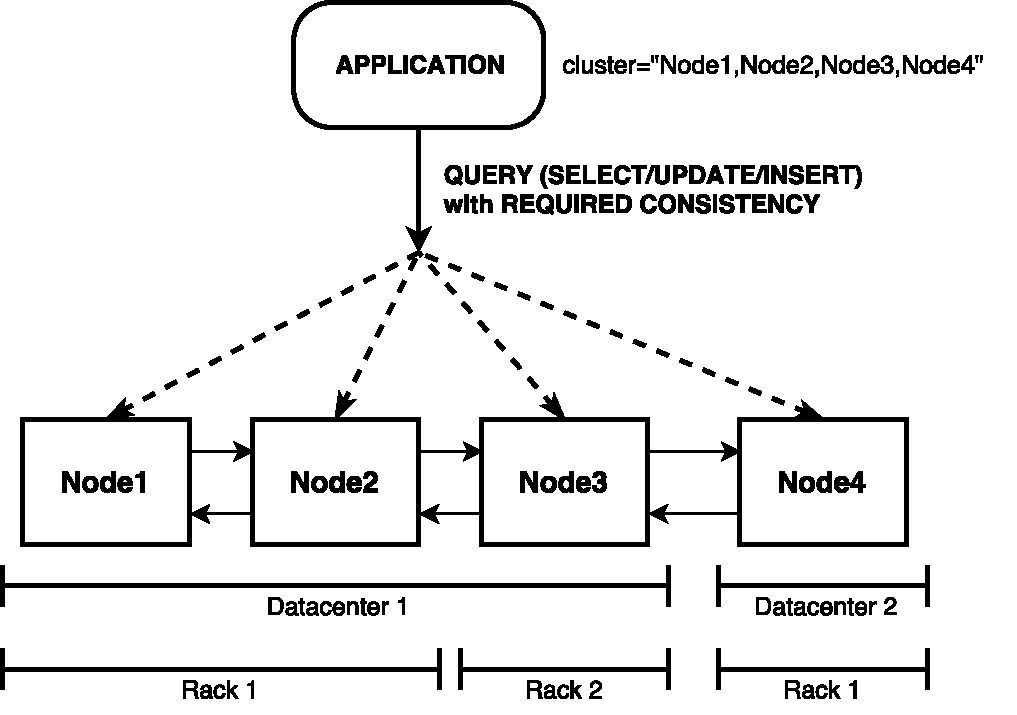
\includegraphics[width=0.7\linewidth]{Figures/cassandra_arch}
    \caption{An overview of Cassandra Architecture}
    \label{fig:cassandraarch}
\end{figure}


Cassandra's architecture revolves around all of the cluster nodes being equal, thus eliminating the need of a master-slave architecture which implicitly introduces a point of failure in the availability. Cassandra’s design was influenced by \textbf{Staged Event-Driven Architecture}, SEDA. \textbf{SEDA} is a general architecture for highly concurrent Internet services \cite{Welsh:2001:SAW:502059.502057} where a single operation may start with one thread, which then hands off the work to another thread, which may hand it off to other threads. Work is subdivided into what are called stages, basic units of work, and the thread pool associated with the stage determines execution. This design means that Cassandra is better able to manage its own resources internally because different operations might require disk I/O, or they might be CPU-bound, or they might be network operations, so the pools can manage their work according to the availability of these resources.

\paragraph{Data Center \& Racks} Cassandra is frequently used in systems spanning physically separate locations. Cassandra grants the possibility to describe the topology of a cluster with two levels of grouping: data center and rack. A \textit{rack} is a set of nodes in proximity to each other, being on the same physical machines or in a single rack of equipment, while a data center is a set of racks, connected by reliable network and located in the same building. Out of the box, Cassandra uses the information provided by the the cluster’s topology described in the configuration to determine where to store data and how to route queries efficiently. In order to maximize availability and partition tolerance, Cassandra stores replicas of data in multiple data centers but tend to favour the use of local nodes to route queries to maximize performance.

\paragraph{Partition Tolerance \& Node Communication} Cassandra uses a gossip protocol so that every node is able to keep track of state information about the other nodes in the cluster, so that decentralization and partition tolerance are supported in a robust way. \textbf{Gossip protocols} (also called “epidemic protocols”) generally behave by assuming a faulty network, within very large, decentralized network systems. They are often used for automated  replication in distributed databases.
A gossiper usually tries to communicate with every endpoint in the cluster, to determine if any of them is dead. It then \textit{convicts} any non-responding endpoint by marking it as dead in its local list, additionally logging that fact.
Failure detection is robustly supported through the \textbf{Phi Accrual Failure Detection algorithm} \cite{hayashibara2004spl}, which is based on the ideas that failure detection should be flexible, decoupling it from the monitored application, and that a traditional heartbeat approach is naive and should be improved via a \textit{suspicion level}, the level of confidence of an actual node failure.
An additional component in Cassandra architecture is the \textbf{Snitch}, which is used to determine relative host proximity in a cluster and gather information about network topology to efficiently route requests, either writes or reads. In its dynamic implementation, it uses a proper version of the Phi failure detection mechanism used by gossipers.

\paragraph{Consistency Levels} Cassandra's tunable consistency make it so that database performances could span from a strong consistency, where each node need to acknowledge each write, to weak consistency, where a single node is sufficient to confirm a write. A consistency level is specified for each read or write query: the higher level of consistency the higher number of nodes or replicas must be acknowledged to the client. Levels go from \texttt{ANY}, \texttt{ONE}, \texttt{TWO} and \texttt{THREE}, considered weak consistency, to \texttt{QUORUM} and \texttt{ALL}, considered strong.

\paragraph{Caching and Tables} Cassandra stores data both in memory and on disk to provide both high performance and durability. When a write operation is performed, it’s immediately written to a \textbf{commit log}, a mechanism for crash-recovery to support Cassandra’s durability goals. A write will not be considered successful until it’s written to the commit log to ensure that, if a write operation does not make it to the \textbf{Memtables}, the in-memory store, it will still be possible to recover the data. 
\\Each memtable contains data for a specific table and when the number of objects stored in the memtable reaches a threshold, the contents of the memtable are flushed to disk in a file called an \textbf{SSTable}, a compacted representation of the memtable, creating then a new memtable.

Cassandra provides three different caches: the \textbf{key cache}, storing a map of partition keys to row index entries, to allow faster read access into SSTables stored on disk; the \textbf{row cache}, containing entire rows, that can greatly speed up read access for frequently accessed rows, at the cost of more memory usage, and the \textbf{counter cache} used to improve counter performance by reducing lock contention for the most frequently accessed counters.

\paragraph{Storage} Cassandra's component to determine how data is distributed across the nodes in the cluster is the \textbf{partitioner}. Exploiting the fact that each row has a partition key, used to identify the partition, it uses a hash function for computing the token of a partition key. Each row is then distributed within the cluster according to the value of the partition key token. Furthermore, each node serves as a replica for different ranges of data: Cassandra replicates data across nodes transparently to the user, via a \textbf{replication factor} specified, that is the number of nodes in the cluster that will actually receive copies of the same data.
The orchestration of Cassandra's storage management is done through internal control mechanisms such as the \textbf{Storage Engine}, which manages all aspects of table storage, including commit logs, memtables, SSTables, and indices.

\subsection{Data Model \& CQL}

With respect to classic relational database design principles, which favours a normalized design of the database, in order to efficiently design a data model in Cassandra, it must be taken into account that \texttt{JOIN}s cannot be performed on Cassandra and that there's no concept of referential integrity. It's favourable to use denormalized tables, modelled with a \textit{Query-first design}, with storage and sorting being design decisions.\\
\\
The basic Cassandra data structures are \textbf{columns}, \textbf{rows}, \textbf{tables}, \textbf{keyspaces} and \textbf{clusters}. The \textbf{column} is the most basic unit of data structure in the Cassandra data model, containing a name and a value of a particular type specified when the column is defined. Each column value contains \textbf{timestamps}, generated each time a value is updated, used by Cassandra to keep data current. In addition, a \textbf{Time To Live} can be configured to guarantee data deletion after the specified amount of time. A \textbf{row} is a container for columns, referenced by a primary key, a uniquely identifying column value. A \textbf{table} is a container for an ordered collection of rows, each of which is itself an ordered collection of columns. The ordering is determined by the columns, which are identified as keys. A \textbf{keyspace} is the outermost container for data in Cassandra, corresponding closely to a relational database. In the same way that a database is a container for tables in the relational model, a keyspace is a container for tables in the Cassandra data model. Like a relational database, a keyspace has a name and a set of attributes that define keyspace-wide behavior, while a \textbf{cluster} is a container for keyspaces that spans one or more nodes.\\
\\
Cassandra offers a SQL-like expressive query language, which supports all of the typical operations that can be done on a relational database, from creating tables and keyspaces, through \texttt{CREATE} queries, to \texttt{INSERT}ions and \texttt{UPDATE}s. The creation of a table must specify a type for each column name: types range from numeric data types (\texttt{int, bigint, smallint, tinyint, varint, float, double decimal}) to text types (\texttt{\justify{text, varchar, ascii}}) and time and identity data types (\texttt{timestamp, date, time, uuid, timeuuid}), but include also simple data types such as \texttt{boolean}, \texttt{blob}, binary large objects, \texttt{inet}, \texttt{counter} and collections such as \texttt{set}, \texttt{list} and \texttt{map}.

Users can define inside each keyspace custom types, composing them with the aforementioned basic types, making sure that if a collection type is used in a User Defined Type, it should be marked as \textit{frozen}, a forward compatibility flag introduced to make sure that individual attributes will be accessible with an \textit{unfreeze} mechanism, once Cassandra will support it.
\chapter{Data Ingestion}

When it comes to using data coming from one or more sources, being them sensors or user activities from a website, there needs to be adequate tools for handling, gathering and routing them inside the cluster where they will be processed.

\section{Kafka}

\textbf{\href{https://kafka.apache.org}{Apache Kafka}} \cite{kafka_doc} is a distributed streaming platform which allows publishing and subscription to streams of records, similarly to a message queue or messaging systems, while storing those streams in a fault-tolerant way and optionally processing them as soon as they enter the system. 

It is mainly used for building real time streaming data pipelines that need to reliably get data between systems or applications, but also when real time streaming applications need to transform or react to the streams of data.

Kafka is run on one or more servers as a cluster, storing streams of \textit{records} in categories called \textit{topics}. Each record consists of a key, a value and a timestamp.

It has two main core APIs, \textbf{Producer and Consumer API}, the basic blocks to create streams, but it's possible to use two more sets of APIs: the \textbf{Streams API}, which can be used to process the records and transform them between two or more topics, and the \textbf{Connect API}, which allows to run producers and consumers that connect to other applications or data systems.

\subsection{Topics}

A topic is a category or feed name where records are published. Topics in Kafka are always multi-subscriber, since a topic can exist regardless of the actual consuming of its records, with zero, one, or many consumers that subscribe to the data written to it.

For each topic, the Kafka cluster maintains a partitioned log, where each partition is an ordered, immutable sequence of records that is continually appended to. A sequential id number called \textit{offset} is assigned to each record within a partition as a unique identifier.

The Kafka cluster, through a configurable retention period, retains all published records, whether or not they have been consumed, so that if, for example, the retention policy is set to three days, then a published record is available for consumption for the following three days, after which it will be discarded to free up space. Taking this into consideration, Kafka's performance is constant with respect to the size of the data stored, causing no actual concern if data need to be stored for a long time.


\begin{figure}[h]
    \centering
    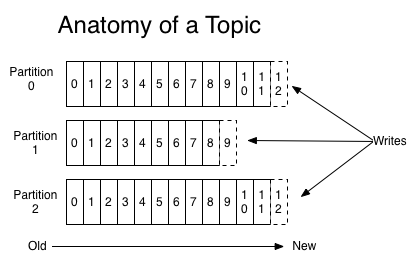
\includegraphics[width=0.7\linewidth]{Figures/log_anatomy}
    \caption[How partition works in a kafka topic]{How partitioning works in a kafka topic. Source: \cite{kafka_doc}}
    \label{fig:loganatomy}
\end{figure}

Only the offset or position of a consumer is retained as metadata, on a per-consumer basis. This offset is completely controllable by the consumer, so that if normally it would advance linearly, the consumer could consume records in any possible order. For example, a consumer can reset to an older offset or, conversely, skip ahead to consume data from the latest record, according to its own policy.

The partitions in the log allow for scaling beyond a size that could fit on a single server, since a topic can handle an arbitrary amount of data, but each individual partition must fit on the servers that host it, and act as the unit of parallelism, so that it's possible to increase the number of partitions of a topic as needed, according to the required throughput.

\subsection{Producers and Consumers}

\paragraph{Producers} They are the components that publish the data to the topics of their choice. They handle the assignment of each record to the partitions within the topic. This is usually done according to a round-robin scheduling, to favour balance loading, or otherwise with a semantic partition function (e.g. the key of a record).

\paragraph{Consumers} They are labelled with a \textit{consumer group} name, and each record published to a topic is consumed by one consuming instance within each subscribing consumer group. Each instance can be in separate processes or even on separate machines.

A common configuration has topics with a small number of consumer groups, one for each "logical subscriber", where each group, for scalability and fault tolerance purposes, is composed of many consumer instances.

\begin{figure}[h]
    \centering
    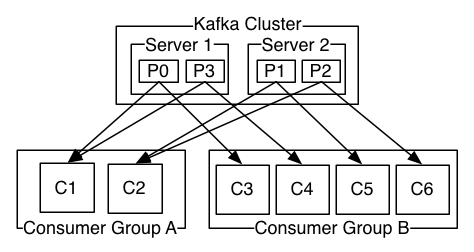
\includegraphics[width=0.7\linewidth]{Figures/consumer-groups}
    \caption[Consumer groups subscribing to a Kafka Cluster]{Consumer groups subscribing to a Kafka Cluster. Source: \cite{kafka_doc}}
    \label{fig:consumer-groups}
\end{figure}


The way Kafka implements consumption is by dividing up the partitions in the log over the consumer instances so that each instance gets a "fair share" of partitions reserved at any point in time. If new instances join the group, Kafka will handle dynamically this addition by giving away some partitions from other members of the group, in order to preserve the fair sharing. Otherwise, if an instance dies, its partitions will be distributed to the remaining instances.

A total order over records is provided only within a partition, and not between different partitions in a topic. However, if a total order over records within a topic is required, than a single partition is needed, consequently meaning that there can only be one consumer process per consumer group. 

\subsection{Use cases}

\paragraph{Messaging}

Kafka can be used as a replacement for a more traditional message broker, for reasons such as decoupling processing from data producers and buffering unprocessed messages. In comparison to most messaging systems, Kafka provides replication, better throughput, built-in partitioning and fault-tolerance, being then a very good solution for large scale message processing applications.

In this domain, Kafka can be compared to  \href{https://www.rabbitmq.com/}{RabbitMQ} and \href{http://activemq.apache.org/}{ActiveMQ}, two of most used traditional messaging systems.

\paragraph{Log Aggregation}

Log aggregation usually collects log files off servers and puts them in a central place, such as a file server or HDFS, for processing purposes. Kafka gives a cleaner abstraction of log or event data as a stream of messages, abstracting away the details of files and allowing, in addition, for lower-latency processing and easier support for multiple data sources and distributed data consumption. In comparison to log-centric systems like Flume, Kafka offers a much lower end-to-end latency and stronger durability guarantees due to replication, while providing equally good performances. 
 
\paragraph{Activity Tracking \& Metrics}

The original use case for Kafka was to rebuild a user activity tracking pipeline as a set of real time publish-subscribe feeds. Thus decomposing site activity, such as page views, searches, or other actions users may take, publishing records to one topic per activity type. These feeds would be available to subscription for real time processing or monitoring, and loading into any data warehousing system for offline processing and reporting.

Kafka is often used for aggregating statistics from distributed applications in order to produce centralized feeds for operational monitoring purposes, providing a fault-tolerant monitoring pipeline with low latency.


\section{NiFi}

\textbf{Apache NiFi} \cite{nifi_doc} is a distributed system for centralising, processing and distributing streams of data across a cluster. Its most notable feature is a web GUI allowing to visually structure the data flow directly from the sources through the definition of graphs where each vertex is called \textbf{Processor} and each edge in-between is a queue in which the \textbf{Flowfiles}, objects wrapping a single records, wait if the processor is busy.

NiFi allows for the creation of a secure cluster where each node takes care of processing a fraction of the Flowfiles circulating inside the graph, load balancing in case of node failures. 

\subsection{FlowFiles}

A \textbf{FlowFile} represents a single piece of data in NiFi, made up of two components: \textbf{FlowFile Attributes} and \textbf{FlowFile Content}. The FlowFile Content is the actual payload, the data that is represented by the FlowFile, while the attributes are characteristics that provide information or context about that data, consisting of key-value pairs. 

All FlowFiles have the following standard attributes:

\begin{itemize}
    \item \textbf{uuid}: A unique identifier for the FlowFile
    
    \item \textbf{filename}: A human-readable filename that may be used when storing the data to disk or in an external service
    
    \item \textbf{path}: A hierarchically structured value that can be used when storing data to disk or an external service so that the data is not stored in a single directory, that is its location on the system
\end{itemize}

\subsection{Processors}

As already mentioned a \textbf{Processor} is the basic block for the graph structure of a NiFi flow. There are a great variety of Processors built in, ranging in function from database connections for insertions or queries to producers and consumers for queue processes such as Kafka; from object manipulation such as JSON or XML splitting and fetching to ingestion from sources like web sockets or filesystems.

A single processor can be scheduled to run periodically or continuously and can be configured with the number of concurrent threads that can be used for the execution. Each Processor has different output ports according to the results of the Flowfile processing: \textit{success}, \textit{failure} or other processor-specific routes (e.g. \textit{\textbf{SplitText}} processor, used to split text according to user-specified rules has \textit{original} and \textit{splits} as additional output ports, used to convey in different routes Flowfiles both before and after being split).
\chapter{Elaborazione Dati}

Una volta che il dato è stato memorizzato, strutturato in maniera conforme al tipo di operazione cui sarà soggetto e pulito è il momento che venga utilizzato attivamente.\\
Questo avviene tramite analisi e elaborazioni operate con il supporto di molteplici framework di sviluppo, aventi come fine ultimo l'estrazione di ulteriori informazioni e la trasformazione di ciò che si è ottenuto finora. Solo in questo modo potranno emergere ulteriori aspetti e \textit{insights}, che verranno visualizzate secondo i dettami della Data Visualization.\\

\section{Le Tecniche}

\subsection{Batch Processing} \label{BatchProc}
Batch data processing is the most classical data processing mode and is characterised by the delayed execution and the simultaneous processing of data in chunks (batches) loaded from a dataset.
\\
\newline
The processing is divided in three phases: at first data are collected for an extended period of time, after which the batch of collected data is loaded to the processing component where it is modified concurrently as a whole, with transformation like Map and Reduce; finally the processed batch is written again on the destination storage.
\newline
\\
The main advantages of this method are that it efficiently processes high volumes of data and transactions, and that processing can be scheduled at fixed times or when the machines' load is light; the main drawback is that it is not suited for real time applications which are becoming more and more prominent.

\subsection{Graph Processing} \label{GraphProc}

A graph in data science is a representation of entities and their relationships.\newline
Entities are represented as nodes, the vertices, and the relationships as edges between those nodes.\newline
\\
Data represented in such way is useful to represent information where connection is as important as the entity, such as people's friends networks or the world wide web; and requires a very different processing model with respect to other structured data.\newline
\\
A widely used Graph processing system is Apache Giraph used for Facebook friends' networks, which implements the architecture described in Google's project Pregel paper for large-scale graph computing\cite{Malewicz:2010:PSL:1807167.1807184}.
\\
Both Apache Spark and Flink feature plugins for the support of graph analysis.

\subsection{Stream Processing} \label{StreamProc}

Streaming data processing differentiates itself from the classic data processing for its use of unbounded datasets, that is a continuous and endless data flow which needs adequate abstractions in order to be able to apply operators or transformations like Map, Reduce and Filter operations. \\ 

Generally, there are 2 execution models usable when approaching an unbounded dataset:

\begin{itemize}
    \item \textbf{Streaming}: continuous elaboration as long as data are being produced.
    \item \textbf{(Micro-)Batch}: finite time execution, which releases resources when the batch processing ends.
\end{itemize}

A Batch based execution is feasible when requirements on the state management, in-order consuming and windowing are not present or very relaxed and, thus, a Streaming approach is generally favoured because of the conceptual paradigm which defines it: \textbf{Dataflow Programming}.

\paragraph{Dataflow Programming}  \label{DataflowProg}

Dataflow Programming is a programming paradigm which models an application as a Direct Acyclic Graph (DAG) and thus it differentiates itself very heavily from the Imperative Programming (or Control Flow), which models a program like finite sequence of operations.\\
This paradigm emphasizes the continuous flow of data between operators, defined as Black Boxes with explicit input and output ports used to connect with other operators. An operation runs as soon as all of its inputs become valid. Thus, dataflow languages are inherently parallel and can work well in large, decentralized systems \cite{Johnston:2004:ADP:1013208.1013209}.

\pagebreak

\section{MapReduce} \label{MapReduce}

\textbf{MapReduce} \cite{hadoop_doc} is a framework, part of Apache Hadoop, named after its processing  abstractions, engined to be run on YARN to deploy applications able to process data in batches from HDFS or distributed databases. \\

\subsection{Structure}
The framework's management is handled by two tracker components, the \textbf{Job Tracker} who acts as a master and the \textbf{Task Trackers} who run on the single nodes, acting as slaves and carrying out the tasks issued by the \textbf{Job Tracker}.

The \textbf{Job Tracker} manages available resource and the MapReduce job's lifecycle.\\ It is responsible for the load distribution using a Data Locality policy, so that nodes are chosen to process data present in their file system if possible or at least from a machine in the same rack. This way the overhead caused by the sending of data is minimised.
\\
The \textbf{Job Tracker} is also responsible for the framework fault tolerance, checks the liveness of tasks and nodes and reschedules failed tasks.

\subsection{Process Flow}

A MapReduce job usually involves six steps:

\begin{enumerate}
	\item \textbf{Load dividing}: The framework elects some nodes to load the Map function and some others to load the Reduction function.
	\item \textbf{Input handling}: The framework divides the whole data set in batches and formats the input to the appropriate key, value pair; each batch is sent to a node marked with a Map for processing.
	\item \textbf{Mapping}: Each Map node applies the Map function defined by the developer to the list of key, value pair in its batch and outputs a transformed list of key, value pairs
	\item \textbf{Shuffling}: The framework sorts and shuffles the pairs output by the Mapping so that pairs with the same key are sent to the same Reduce node.
	\item \textbf{Reducing}: Each Reduce node applies the Reduce function defined by the developer to the Mapped list of key, value pair and for each key aggregates all values and produces one or more transformed pairs.
	\item \textbf{Output handling}: The framework collects all outputs from Reduce nodes and writes it onto HDFS or a DB, usually the same where the input data set came from.
\end{enumerate}

 \pagebreak
 
\section{Apache Spark} \label{Spark}

Apache Spark è un framework open source per il calcolo distribuito in tempo reale, nato a Berkeley nel 2009 e successivamente passato sotto l'ala della Apache Software Foundation, che si occupa tuttora del suo mantenimento.\\ Grazie alle sue caratteristiche ha un ampio spettro di applicazioni, dal Batch Processing al Graph Processing e Stream Processing.
\subsection{Requisiti} 
Il framework richiede un'ambiente che lo supporti nell'interazione con il resto dell'architettura: un gestore di cluster e un sistema di archiviazione distribuita.\\ 
Per quanto riguarda il primo sono supportati Hadoop YARN o Apache Mesos, in aggiunta ai quali è possibile adottare l'opzione \textit{standalone}, consigliata solo con obiettivi di testing, in cui è Spark che avvia il singolo nodo su cui eseguire l'applicazione. In ogni caso il framework è completamente astratto da questo aspetto, unificando l'approccio per ogni scelta adottata.\\
Per il secondo punto il framework richiede uno tra cui i principali rappresentanti della categoria, tra i quali i già citati HDFS o Cassandra.\\ 

\subsection{Architettura}
Spark adotta un'architettura distribuita di tipo "Master Slave": un task \textit{Driver} e molteplici tasks \textit{Worker}.\\ 
Il programma \textit{Driver} viene eseguito sul nodo principale e gestisce la divisione delle operazioni sugli altri nodi tramite l'oggetto \textit{SparkContext}. Questo interagisce con il gestore del cluster del sistema per definire job \textit{Executors} nei nodi secondari. A questi vengono successivamente inviati il codice dell'applicazione e i task particolari da eseguire.\\
I programmi \textit{Worker} vengono avviati sui nodi secondari e rimangono in esecuzione per tutta la durata dell'applicazione. È importante sottolineare che ogni applicazione genera processi indipendenti dalle altre, garantendone l'isolazione reciproca per lo scheduling. Tuttavia ciò significa che l'unico modo per far comunicare applicazioni in esecuzione contemporanea consiste nella scrittura su memoria esterna.\\

\begin{figure}[h]
	\centering
	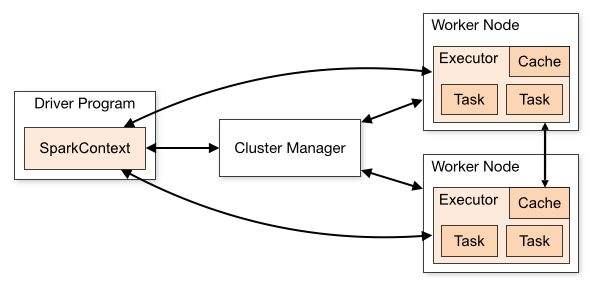
\includegraphics[scale=0.75]{Figures/spark_architecture.png}
	\decoRule
	\caption[Architettura Spark]{Architettura Master Slave}
	\label{fig:Architettura Spark}
\end{figure}

\subsection{Caratteristiche}
Spark si pone nel panorama del Data Processing come principale concorrente ad Hadoop MapReduce. Infatti, contrariamente alla controparte, fornisce l'opzione per lo Stream Processing e punta sull'analisi in tempo reale.\\
Per fare ciò l'architettura utilizza primitive "in-memory", lavorando direttamente in RAM laddove possibile. Questo approccio riduce di molto i tempi di latenza, rimuovendo l'overhead della scrittura su disco. Proprio per queste caratteristiche Spark viene preferito per algoritmi di apprendimento automatico e analisi dati interattiva, che richiedono accesso ripetuto agli stessi dati. \newline
<grafico prestazioni mapreduce vs spark>

\subsection{Struttura}
Il framework è organizzato su due livelli di librerie. Quello fondamentale è costituito da SparkCore, che fornisce i metodi e strutture dati principali e su cui poggiano le estensioni più specifiche:
\begin{itemize}
	\item SparkSQL
	\item Spark Streaming
	\item MLlib (Machine Learning Library)
	\item GraphX
\end{itemize}  

\begin{figure}[h]
	\centering
	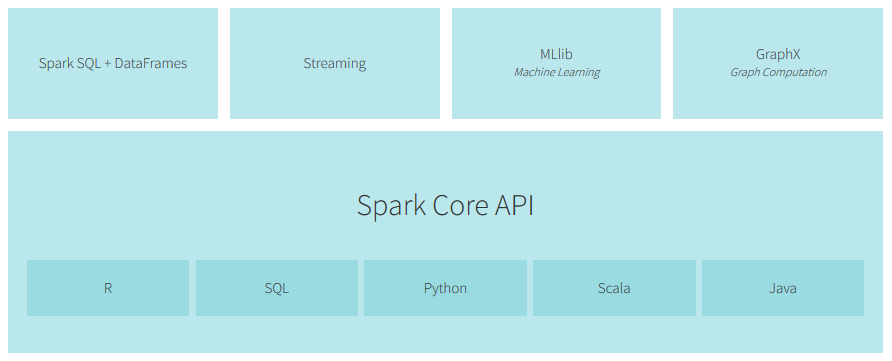
\includegraphics[scale=0.75]{Figures/spark_structure.png}
	\decoRule
	\caption[Struttura Spark]{Struttura Spark}
	\label{fig:Struttura Spark}
\end{figure}

\subsubsection{SparkCore e RDD}
SparkCore costituisce le fondamenta dell'intero framework. Garantisce la distribuzione dei task, lo scheduling e funzionalità di input e output di base. Tutte questo orbita intorno all'astrazione fornita dai RDD (Resilient Distributed Dataset), una struttura dati immutabile, tipata e distribuita sui nodi del cluster. Questa utilizza una politica di "fault tolerance" basata sul mantenimento delle operazioni che hanno interessato il singolo RDD, in modo che esso possa essere ricostruito in caso di criticità a partire da queste informazioni. \newline
Coerentemente con la filosofia del framework, gli RDD lavorano "in-memory" per quanto possibile e, se necessario, vengono persistiti in memoria o su disco. Essi rispondono al paradigma "Trasformazione/Azione" per ottimizzare l'esecuzione delle operazioni: 
\begin{itemize}
	\item Trasformazioni, le operazioni che cambiano la forma in qualche modo del RDD (per esempio Map, Filter) e valutate in maniera "lazy", ossia effettuate solo nel momento in cui un'Azione prende atto
	\item Azioni, le operazioni che accedono al RDD per restituire un risultato tipato
\end{itemize}
L'accesso ai metodi della libreria SparkCore viene fornito tramite la classe SparkContext, tramite cui è possibile creare RDD a partire da dati in locale o su HDFS.

\subsection{Extensions}
\subsubsection{GraphX}

GraphX is a Spark extension for graphs and graph analysis. GraphX extends RDD adding a Graph abstraction implemented as a directed multigraph with properties attached to both vertices and edges and exposes typical graph operators, while also providing an optimized variant of the Pregel API.

\paragraph{Property Graph}

The Graph abstraction, or property graph is a directed multigraph with properties attached to each vertex and edge, defined by the developer. A directed multigraph is defined as a directed graph where more than one edge can connect two nodes, as two nodes might have multiple relationships with different properties, (e.g. Annie and Barb are both colleagues and friends). \\ \\
Property graphs, like RDDs, are immutable and to transform them a new one must be instantiated from the former through an operation, they are distributed across executors using vertex partitioning heuristics and are fault-tolerant, thanks to the same lineage mechanism seen in RDDs.

\paragraph{Graph Operations}

Graphs implement several operators that can be divided in three classes:

\begin{itemize}
	\item \textbf{Property Operators}: the Graph equivalent to RDD map, with the difference that you can choose to map over the vertices, the edges, or the \texttt{<source node, edge, destination node>} triplets , to modify the properties of said components.
	\item \textbf{Structural Operators}: acting on the topology of the graph, an example would be reverse which, from a Graph, returns a new Graph where all edges' directions are reversed.
	\item \textbf{Join Operators}: used to join properties from different graphs or from external collections like RDDs.
\end{itemize}


\subsubsection{SparkStreaming}

\textbf{SparkStreaming} is a Spark extension developed to enable live data stream processing in the fault-tolerant and highly scalable framework provided by Spark while maintaining a high throughput.
The ingested stream source can be any major source like Kafka, Flume and NiFi; other streams like Amazon Kinesis, filesystems like HDFS or S3 and TCP sockets.
The stream can be processed through the high-level functions like map, reduce and join and finally output to any filesystem, distributed databases or further stream outputs.

\paragraph{DStream}

DStream, short for Discretized Stream, is the main abstraction introduced by SparkStreaming, which represents a continuous stream of data. \\
As for RDDs, DStreams can be instantiated from a stream source like Kafka, Flume and Kinesis, or by applying a transformation on another DStream like map. As it stands, DStreams are in fact sequences of RDDs, maintaining therefore their properties of being distributed and fault-tolerant.
\\ \\
Internally a continuous stream of data, DStream splits the live flow into mini batches which are then sent to the Spark engine that can then process them as batches and output them to processed batches as previously seen.

\subsubsection{MLlib}

Machine Learning Library, or \textbf{MLlib} for short is a set of APIs for Spark that exposes several tools for Machine Learning, using Spark as a backend taking advantage of Spark's efficiency in iterative algorithms.

MLlib exposes a selection of Machine Learning algorithms for classification, regression, creation of decision trees and random forest, recommendation, clustering, topic modelling and pattern mining.
It also offers other tools to transform features, to handle datasets and hyperparameters and to make computation with distributed linear algebra and statistics.

\pagebreak
\section{Flink}\label{Flink}

\href{https://flink.apache.org/}{\textbf{Apache Flink}} \cite{flink_doc} is an open source framework developed for the continuous and distributed processing of data flows. Based on the Dataflow Programming model, it provides a set of abstractions specifically designed for real time stream processing.

\subsection{Abstraction levels}  \label{AbstractionLevels}

\begin{itemize}
	\item \textbf{Stateful Streaming}: It's the lowest abstraction layer, which allows developers to freely manage data flows and their processing, use fault-tolerant states and callback registration on events.
	\item \textbf{Core API}: it's the basic API, which is divided between \textbf{DataStream API}, specifically conceived for bounded and unbounded dataset processing, and \textbf{DataSet API}, implemented as a special case of the first API set, used only for bounded datasets. These 2 APIs offer transformations and operations like unions, aggregations, windowing and state management, needed for the data flow upon which they are applied.
	\item \textbf{Table API}: it's a declarative DSL \footnote{Domain Specific Language: a language with a limited expressiveness which focuses on a given domain of use.} which follows the extended relational model and offers the possibility to model a data stream like a table upon which it's possible to execute operations like projections, aggregations and groupings. Despite being less expressive with respect to the Core API, it allows for a greater compactness when it comes to describing the operations to be executed on the data.
	\item \textbf{SQL}: it's the highest level of abstraction offered by Flink and interacts directly with the Table APIs in order to provide a representation of the application being developed through SQL queries. It can be executed on the tables defined by the Table API, thus directly on the data.
\end{itemize}
\pagebreak
\subsection{Programs Dataflows}  \label{ProgramsDataflows}

The base elements of a Flink application are the following:

\begin{itemize}
	\item \textbf{Streams}, data structures containing data.
	\item \textbf{Transformation Operators}, which can change the stream, for example, via aggregations, groupings, mappings and reductions.
	\item \textbf{Sources}, they are primary data entry points and can be files or records from queues like Kafka. They are the starting nodes of the application DAG.
    \item \textbf{Sinks}, They are the application output, being it a file, any process or another queue. They are the ending nodes of the application DAG.
\end{itemize}

\begin{code}

\begin{minted}[breaklines]{Scala}
val lines = env.addSource(new Consumer[String](...))

val events = lines.map(line -> parse(line))

val stats = events
            .keyBy("id") // Stream is partitioned by the key "id" 
            .timeWindow(Time.seconds(10)) // All the events in the given window are considered 
            .apply(MyWindowAggregationFunction()) // All the records are aggregated according to the function      

stats.addSink(new RollingSink(path))
\end{minted}

\end{code}

\begin{figure}[h]
	\centering
	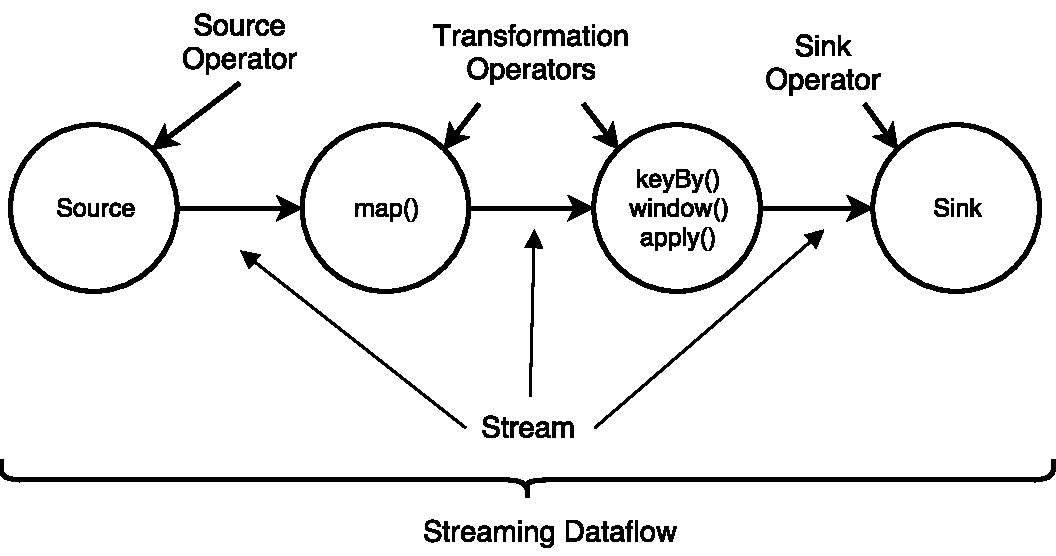
\includegraphics[scale=0.75]{Figures/dataflow.pdf}
	\decoRule
	\caption[Streaming Dataflow]{DAG outlining the previous code snippet}
	\label{fig:Dataflow}
\end{figure}

\paragraph{Event Time}

Flink supports different notions of time in streaming programs \cite{flink_eventtime}, each of them useful for specific use cases:

\begin{itemize}
    \item \textbf{Processing time} refers to the system time of the machine that is executing the respective operation.
    
    When it is being used, the system clock of the machines will be used to run all time-based operations. Being the simplest notion of time, no coordination is required between streams and machines, providing, this way, the best performance with the lowest latency. However, since the entire environment is distributed and might work asynchronously, processing time does not provide determinism, because of its susceptibility to the speed at which records arrive in the system and flow between each pair of operators inside the system.
    
    \item \textbf{Event time} is the time embedded within a record, representing when it occurred on its producing device. This time is typically assigned before records enter Flink and it can be extracted directly from the record at the Source level. An event time window of an hour will contain only records carrying an event timestamp within that hour, regardless of their actual time and order of arrival.
    
    Event time is especially useful when dealing with out-of-order or late events, and even on replays of data from persistent logs or backups. When using event time, the progress of time is discretized based on the data, rather than the clock, and the generation of the Event Time Watermarks, central to the mechanism that signals progress in event time,  must be specified internally to the program.
    
    Event time processing inherently causes a certain latency, due to its waiting for late and out-of-order events.
    
    \item \textbf{Ingestion time} is the time that events enter Flink. The source operator assigns to each record its current time as a timestamp, which all time-based operations refer to.
    
    Ingestion time can be considered an alternative, conceptually speaking, in between event time and processing time: it is more expensive than processing time, while providing deterministic results, as it uses stable timestamps assigned once at the source and used by all of the following time-based operations, but cannot handle any out-of-order events or late data, with respect to event time, even though there's no need to specify the watermarks generation.
\end{itemize}


\paragraph{Windows}

Windows are the core mechanism within a stream processing framework. They allow the application of operations after splitting the stream into \textit{buckets} of finite size. The structure of a windowed Flink program differs when considering \textbf{keyed} and \textbf{non-keyed} streams: a keyed stream is split into multiple logical sub-streams and a window is applied to each one of them separately, differently from a non-keyed stream where the window is applied globally and within a single task \cite{flink_windows}.

A Window lifecycle starts as soon as the first element belonging to it arrives, ending, by being completely removed, when the time, event or processing time, passes its end timestamp plus any user-specified \textbf{allowed lateness}. For example, in an event-time-based Flink application where a tumbling window is created every 5 minutes with an allowed lateness of 1 minute, a new window will be created for the interval between 11:30 and 11:35, as soon as a record with a timestamp falling into that interval arrives, and will be removed when the watermark passes the 11:36 timestamp.

For each window must be specified a \textbf{Trigger} and a function (\texttt{WindowFunction}, \texttt{ReduceFunction} or \texttt{FoldFunction}) attached to it: the Trigger is used to specify the conditions under which the window is considered ready or complete for the function to be applied, while the function will contain the operation to be applied to the contents of the window. The triggering policy is completely customizable and can even decide to purge a window’s contents, leaving the window metadata untouched, in order to add new data to that window.

It's possible specify an \textbf{Evictor}, used to remove elements from the window after the trigger fires and before and/or after the function is applied.

There are four main window assigners usable in Flink:

\begin{itemize}
    \item \textbf{Tumbling Windows} are fixed size and non-overlapping windows, configured with a parameter controlling how much frequently a new window has to be started.
    \item \textbf{Sliding Windows} are fixed size, similarly to tumbling windows, but are configured with an additional slide parameter, which controls how frequently a sliding window is started. Therefore they may overlap, with elements assigned to multiple windows.
    \item \textbf{Session Windows} group elements by sessions of activity. Session windows do not overlap and do not have a fixed start and end time, in contrast to tumbling windows and sliding windows. A session window closes when it does not receive elements for a certain period of time, i.e., when a gap of inactivity occurred.
    \item \textbf{Global Windows} assign all elements with the same key to the same single global window. This windowing scheme is only useful if you also specify a custom trigger. 
\end{itemize}



\paragraph{Parallelism} \label{ParallelismFlink}

Applications using Flink are inherently parallels and distributed. During execution, a stream may be divided in more than one partition; each operator can have more than a single sub-task operating on data, each one independent from the other and executed on different threads or, if possible, on different machines or containers.\\
The parallelism of a task is the parameter indicating the number of subtasks an operator can have and, consequentially, the number of partitions of the stream getting outputted from that operator.\\

\begin{figure}[!htb]
    \centering
    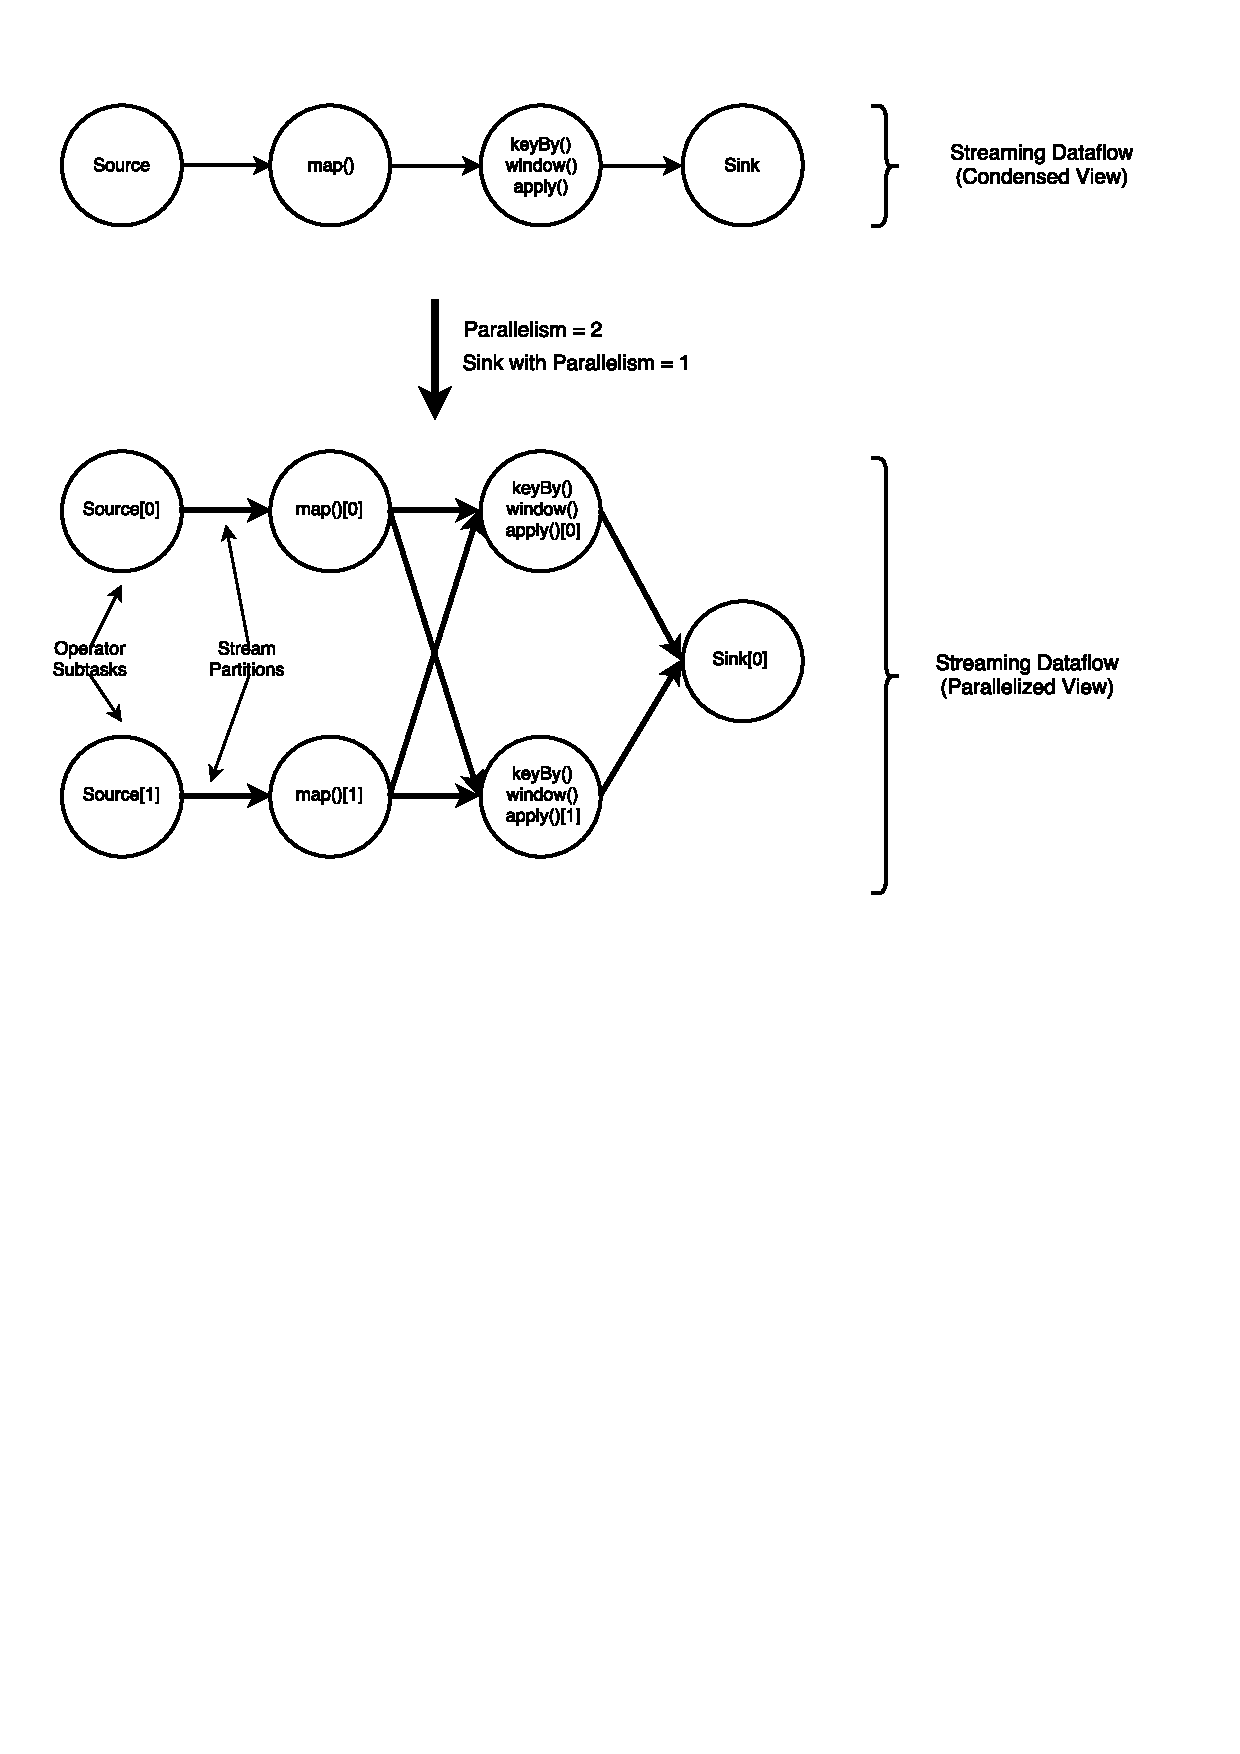
\includegraphics[scale=0.75, trim=0.5cm 12cm 1cm 0.5cm]{Figures/parallel_dataflow.pdf}
    \decoRule
    \caption[Parallel Dataflow]{DAG with Parallelism=2}
    \label{fig:ParallelDataflow}
\end{figure}

Streams can transport data between a pair of operators following two different patterns: One-to-one pattern and redistributing pattern:
\begin{itemize}
	\item \textbf{One-to-one streams} preserve the stream partitioning and the order of the elements passed to the following operator. For example, the subtask[0] of a \texttt{map()} operator will get to see the same elements produced by the subtask[0] of the previous Source operator.
   
    \item \textbf{Redistributing streams} change their partitioning, sending the data to different subtasks, based on the transformation being applied. For example, a \texttt{keyBy()} operator repartitions the stream using the hash of the chosen key. In this case, the elements' order will be preserved only between neighbouring operations pairs, and won't be ever guaranteed being the same in the following operators.
\end{itemize}

\subsection{Data Streaming Fault Tolerance}

Flink offers built-in guarantees in case of failures, so that there's minimum disruption on the processing jobs and a consistent recovery of the data streaming applications' state. The two main features which allows recovery from errors or runtime exceptions are \textbf{Checkpoints} and \textbf{Savepoints}.

In case of a program failure (due to machine-, network-, or software failure), Flink stops the distributed streaming dataflow, restarting the operators and resetting them to the latest successful checkpoint, while also resetting the input streams to that same point of the state. Any records processed as part of the restarted parallel dataflow are guaranteed to not have been part of the previously checkpointed state.

For this mechanism to realize its full guarantees, the data stream source needs to be able to rewind the stream to a defined recent point. Apache Kafka, thanks to its offsets, has this ability and Flink’s connector to Kafka makes use of it.

\subsubsection{Checkpoints}

\begin{code}
    \label{code:checkpointing}
    \begin{minted}[breaklines, breakbefore=., breakafter=(]{Scala}
    val env: StreamExecutionEnvironment = StreamExecutionEnvironment.getExecutionEnvironment
    
    env.enableCheckpointing(60000)
    
    env.getCheckpointConfig.enableExternalizedCheckpoints(ExternalizedCheckpointCleanup.RETAIN_ON_CANCELLATION)
    
    env.setStateBackend(new FsStateBackend(state_dir, true)) 
    \end{minted}
    \captionof{listing}{An example of asynchronous checkpointing configuration on a FileSystem backend}
\end{code}~\\

\textbf{Checkpoints} are Flink's tool to guarantee automatic fault tolerance and recovery of the job's state, in case of runtime errors or failures \cite{flink_checkpointing}. 
\\
\\
They are, essentially, snapshots of the current state of the job that act consistently as the system fall back in case of failure. Flink’s mechanism for drawing these snapshots is inspired by the standard Chandy-Lamport algorithm \cite{Chandy:1985:DSD:214451.214456} for distributed snapshots and is specifically tailored to Flink’s execution model \cite{DBLP:journals/corr/CarboneFEHT15}. 
\\
\\
Checkpointing must be configured on the application level as shown in the previous snippet by calling the \texttt{enableCheckpointing(milliseconds)} to specify how much time should pass between two consecutive snapshots. By default, if a job is cancelled the checkpoint is deleted as well, so the retainment on cancellation must be enabled manually. 
\\
\\
An additional configuration available to application level setup is the State Back-end, that is the location where the checkpoint, thus, the job's state, should be saved. There are three possible back-ends which can be chosen from: \textbf{in Memory}, useful for testing, on a \textbf{Filesystem} (local or distributed, like HDFS) and on \textbf{RocksDB}\footnote{\href{http://rocksdb.org/}{RocksDB} is an embeddable persistent key-value store for fast storage}, particularly recommended for huge states. Optionally, snapshots can be taken asynchronously in order not to block the processing pipeline.
Checkpoints can be used to manually recover from failures through specific commands from Flink CLI, but they don't support scaling on recovery, that is, parallelism can't be changed when recovering from a snapshot.

\paragraph{Barriers}

A core element in Flink’s distributed checkpointing are the \textit{stream barriers}: lightweight elements flowing with the records, as part of the data stream, injected into the stream starting from the data source, without interrupting it. They are used to separate the records in the data stream belonging to two consecutive snapshots. Each barrier contains the ID of the snapshot whose records were pushed in front of it: there can be multiple barriers belonging to different snapshots, meaning that checkpoints may happen concurrently.
\\
\begin{figure}[!htb]
    \centering
    \includegraphics[width=1\linewidth]{Figures/stream_barriers}
    \caption{Visual representation of Stream Barriers}
    \label{fig:streambarriers}
\end{figure}
\\
Let's call $S_n$ the point in the stream where the barriers for snapshot $n$ are injected, representing the position up to which the snapshot covers the data, reported to the checkpoint coordinator, Flink’s JobManager.
\\\\
Flowing downstream, each intermediate operator must receive a barrier for snapshot $n$ from all of its input streams before emitting a barrier for the same snapshot into all of its outgoing streams, until a sink operator is reached. Once a sink has received a barrier $n$, from all of its input streams, the snapshot $n$ is acknowledged to the checkpoint coordinator and the checkpoint is considered complete.

At the completion of snapshot $n$, the job will never ask the sources to replay the records from before $S_n$, since they all went through the topology.
\\\\
If an operator receives more than one input stream, an \textit{\textbf{alignment}} step must be performed between all of the inputs:

\begin{itemize}
\item As soon as the operator has received a snapshot barrier $n$ from an incoming stream, it must wait the same barrier from all of the other inputs, since otherwise processing would mix records belonging to consecutive snapshots and, in this case, would use also the barriers for snapshot $n+1$.

\item While waiting, all barriers $n$ are temporarily set aside and the corresponding records put in an input buffer.
    
\item Once the last stream has received barrier $n$, the operator emits all pending outgoing records and then snapshot $n$ barriers itself, before continuing processing records, starting from input buffers and then the actual input streams.
\end{itemize}

\paragraph{Exactly Once vs. At Least Once}

The alignment step previously described may add latency to the streaming program, usually negligible, being in the the order of a few milliseconds, but some applications' latency may increase noticeably. If consistent super low latency (few milliseconds) for all records is a strict requirement, Flink allows to skip the stream alignment during a checkpoint, but snapshots are still drawn as soon as an operator has seen the checkpoint barrier from each input stream.

As a consequence, the operator keeps processing all inputs, including elements belonging to checkpoint $n+1$, which will then occur as duplicates when restoring the state of the stream because they are both included in the state snapshot of checkpoint $n$ and part of the data following this same checkpoint.
\\

The alignment step happens only when operators with multiple predecessors (join operators) or 
multiple senders (such as a stream repartitioning/shuffle) are present. For this reason, dataflows containing only parallel streaming operations (\texttt{map()}, \texttt{flatMap()}, \texttt{filter()}, …) guarantee \textit{exactly once} semantics even in \textit{at least once} mode.

\subsubsection{Savepoints}

\begin{code}
    \label{code:savepoint}
    \begin{minted}{Bash}
flink savepoint <jobId> [<savepointDirectory>] -yid <yarnAppId> 
    \end{minted}
    \captionof{listing}{Savepoint triggering from the Flink CLI}
\end{code}~\\

\textbf{Savepoints}, just like checkpoints, serve the purpose to save the state of a Flink application in case of cancellation or failures. Differently from checkpoints, they can only be performed manually from the Flink CLI, but support parallelism rescaling and they're the go-to choice when Flink's application computational capabilities must be improved by setting an higher parallelism factor or when an upgrade to a more recent version of Flink must be performed. Savepoint's mechanism works such that it associates each application's stateful operator, to its own state in a map-like structure: for this very reason, in order to successfully preserve state when upgrading a Flink application, each stateful operator needs to have its own \texttt{uid} set.

\subsection{High Availability}

A Flink's setup, whether a standalone cluster (being it containerized or physical) or using Distributed Resource Managers such as \nameref{YARN} or Mesos, is made of a Job Manager and one or more Task Managers, each one with one or more parallelism slots (cores usable for processing). Task Managers (TMs) handle jobs actual executions, while the Job Manager (JM) handles TM orchestration and monitoring and, for this reason, is a single point of failure, whose crash causes the entire Flink cluster to stop.
Flink High Availability setup follows the principles of a Active-Standby architecture (also used by HDFS Namenode e YARN Resource Manager HA set-ups) where a single leading JM is active, while multiple JMs standby, ready to take over leadership in case the leader failure. This guarantees that there is no single point of failure and programs can make progress as soon as a standby JM has taken leadership. There is no explicit distinction between standby and master JM instances: all of the possible JMs are registered as masters to \textbf{Zookeeper}, which is going to handle failure scenarios.

In case of YARN clusters configured in High Availability mode, a single JM, the \textbf{Application Master}, is run, but YARN itself will restart its container on failures. As additional configuration, the maximum number of attempts for the application masters needs to be configured in the YARN configuration.

\subsection{Flink Extensions} \label{FlinkLibs}

\subsubsection{FlinkCEP: Complex Events Processing}

FlinkCEP is a Flink extension adding the possibility to analyse events pattern in a DataStream, thanks to the Pattern API. This API allows the definition of patterns to be found in a stream and their selection in order to create a new DataStream of Alerts.\\


\begin{code}
\label{code:pattern-example}
\begin{minted}[breaklines]{Scala}

val inputStream: DataStream[SensorEvent] = ...

val pattern = Pattern.begin("start").where(_.getId == 42)
.next("middle").subtype(classOf[TemperatureEvent]).where(_.getTemperature >= 90.0)
.followedBy("end").where(_.getName == "end")

val patternStream = CEP.pattern(inputStream, pattern)

val result: DataStream[Alert] = patternStream.select(createAlert(_))
\end{minted}
\captionof{listing}{An example of Pattern API usage}
\end{code}~\\

In FlinkCEP, a \textbf{Pattern}, similarly to a pattern of a Regular Expression, can be \textbf{single} or \textbf{iterative}. For example, in a pattern like \texttt{"a b+ c? d"}, \texttt{a}, \texttt{c?} e \texttt{d} are single patterns, while \texttt{b+} is iterative.
\\
In a Pattern there can be, analogously to regular expressions, \textbf{quantifiers} and \textbf{conditions}.

\paragraph{Quantifiers}

Iterative patterns can be specified with the following self explanatory methods:

\begin{itemize}
    \item \texttt{pattern.oneOrMore()};
    \item \texttt{pattern.times(\#ofTimes)};
    \item \texttt{pattern.optional()}
\end{itemize}

\paragraph{Conditions}

Each pattern can have additional conditions specified, which can be related to a property of an incoming event, or the contiguity to other events.

Methods \texttt{pattern.where()} and \texttt{pattern.or()} can be used to specify \texttt{\justify{IterativeCondition}}s, \texttt{SimpleCondition}s or a combination of multiple conditions. In this case, combinations can be specified concatenating all the previous methods, including the quantifiers, optionally adding more constraints on the contiguity of the same pattern by calling \texttt{consecutive()}, for the strict contiguity, and \texttt{allowCombinations()} for the relaxed non-deterministic contiguity.
\\
Some examples:
\\
\begin{code}
\label{code:iterative-cond}
\begin{minted}[breaklines]{Scala}
middle.oneOrMore().where(
    (value, ctx) => {
        lazy val sum = ctx.getEventsForPattern("middle")
                          .asScala.map(_.getPrice).sum
        value.getName.startsWith("foo") && sum + value.getPrice < 5.0
    }
)
\end{minted}
\captionof{listing}{Iterative Condition}
\end{code}~\\

\begin{code}
    \label{code:simple-cond}
    \begin{minted}[breaklines]{Scala}
//Example of conjunction through where concatenation
start.where(event => event getName startsWith "foo" ) )
     .where(event => event getTotal equals 50  )

start.subtype(classOf[SubEvent]).where(subEvent => ... /* some condition */)
    \end{minted}
    \captionof{listing}{Conditions combinations}
\end{code}~\\

\pagebreak

\paragraph{Pattern Combination}

Similarly to conditions combination, pattern combination is possible through the consecutive calls to the following methods allowing to specify the contiguity constraints which a given pattern should satisfy:

\begin{itemize}
    
    \item \texttt{next()}, for strict contiguity.
    \item \texttt{followedBy()}, for relaxed contiguity.
    \item \texttt{followedByAny()}, for non deterministic relaxed contiguity.
    \item \texttt{notNext()}, NOT pattern with strict contiguity.
    \item \texttt{notFollowedBy()}, NOT pattern with relaxed contiguity.

\end{itemize}

Each pattern combination can be followed by a time constraint specified by concatenating \texttt{within(Time)}.

\paragraph{Pattern Detection}

Once a pattern sequence has been specified, it needs to applied to the target \texttt{Datastream}, creating this way a \texttt{PatternStream}.
On this new stream \texttt{select} or \texttt{flatSelect} operations need to be applied in order to enable further processing on the events satisfying the pattern.

\subsubsection{Other extensions: Flink Gelly and FlinkML}

In addition to the aforementioned library for complex event handling, Flink makes available specific sets of API, which provide useful tools when it comes to enable advanced processing on data.

\paragraph{Flink Gelly} is an API based on the Flink \texttt{Dataset}s API specifically developed for Graph Processing. Graphs are stored as a finite set of vertices and edges, a special case of a \texttt{Dataset}. This library allows the application of operators like Map, Filter, Intersect and Union, mutations like edge and vertex removal, but also advanced techniques belonging to Graph Theory like \textit{Iterative Graph Processing} (Vertex-centric, Scatter-Gather and Gather-Sum-Apply), \textit{Single Source Shortest Paths}, \textit{Clustering} and \textbf{Similarity Analysis}.

\paragraph{FlinkML} is a set of tools which allows the application of Machine Learning techniques over Flink data sets, including both algorithmic implementations for supervised (\textit{SVMs} and \textit{Multiple Linear Regressors}) and unsupervised (\textit{K-nearest neighbours}) learning, Data Preprocessing and Recommendation (\textit{ALS}).



\chapter{Data Visualization}

Data Visualization is the visual representation of data using plots and visual models. In the infrastructural stack, it stands at the highest level since it's the mean through which the results of processing are shown to the final user. The reason that makes it so important is that humans are not able to extract useful information from raw data at a glance, and there comes the need for clear and intuitive plots which capture all the helpful statistics contained, in a concise way, from which humans gain insights and act accordingly.

The stack uses as a visualization tool \textbf{Tableau}, and in this chapter will be presented its structure and its strengths. 

\section{Introduction}

Tableau is a software dedicated to the creation of visualisations for the Business Intelligence. Tableau offers an highly intuitive and interactive way to the access, manipulation and analysis of data, without any need for coding, positioning itself among the first three product leaders in the sector \cite{gartner_tableau}. Tableau's main features include easiness and intuitiveness in the software use, data sources management and some innovative features such as table calculations and the possibility to use data analysis techniques directly on the plots.

Tableau On Premise version is composed of two elements:

\begin{itemize}
    \item \textbf{Tableau Desktop}: Allows for the creation of worksheets, dashboards and stories, linked to one or more data sources.
    \item \textbf{Tableau Server}: It is used to publish the plots created with Tableau Desktop, in order to make them available to the end users.
\end{itemize}

\section{Tableau Desktop}

Tableau is structured in a Microsoft Excel fashion, with workbooks and sheets: a \textbf{workbook} is made of many sheets which can be worksheets, dashboards or stories. A worksheet is a single plot, with its own filters and legend, and can be combined with other worksheets to make a dashboard. A story is a sequence of dashboards and it's usually the view shown to the end user. Each workbook starts from one or more data sources, used by Tableau for fetching the data used in the plots.

\subsection{Data Source}

The first step during the creation of a workbook is to link Tableau to a data source \cite{LearningTableau}, either through a \textbf{File Connection}, which supports all of the main data formats available such as JSON, CSV, TSV, PDF and Excel sheets, or a \textbf{Server Connection}, to \textbf{relational databases}, such as Microsoft SQL Server and Hive, \textbf{NoSQL databases}, such as MongoDB or Cassandra, and \textbf{data sources in cloud}, such as Google Analytics, Amazon Redshift and Salesforce. If there's no optimized built-in driver, it's possible to use any ODBC\footnote{ODBC: Open DataBase Connectivity is a standard API to access DBMS} driver. Any interaction with a data source is handled by default with \textbf{VizQL} (Visual Query Language), which translates all of the drag-n-drop actions executed in the GUI to adequate queries to the data source, in order to get the desired results available for visualisation.

Tableau's connection to a data source is available in two different types: Live and Extract.

\paragraph{Live}

A \textbf{Live} connection queries directly the data source, making the performances of this connection strictly dependent from the performances of the database being used. With this kind of connection it's possible to refresh all the plots each time data is being updated, making the visualisations almost real time.

\paragraph{Extract}

An \textbf{Extract} connection is a periodic query, which can be performed, for example, every day, which saves the results in a Tableau Data Extract file, which will be used for all of the following queries. The Extract may be considered a snapshot of the database and, for this very reason, any update in the database won't be seen until the next scheduled Extract File update. Even though the creation of an Extract File can take a long time, queries on it are very efficient because of its internal tabular structure, optimized for Tableau's own execution engine.

\subsection{View Creation}

Each field loaded from the data source is assigned one of two roles: dimension or measure. A \textbf{dimension} is used for categorised or discrete information, such as strings or dates, while a \textbf{measure} corresponds to numeric information, potentially object of aggregations. It's possible to change freely the roles of each field, according to the needs. Drag-n-drop allows to move dimensions and measures on both plots' axes and Tableau is able to automatically interpret the new layout, constructing a more significant chart.

\subsubsection{View Choice}
The main focus of visual analytics is to represent data in a fashion so that it conveys as much information as possible at a glance.
Tableau offers the possibility to create several kinds of visualisations, each one suitable for a specific use case. The three most common charts are without a doubt the bar graph for data comparisons, line graph for trends and pie charts to underline the share of different categories inside a single field.
More advanced representations are also supported such as:

\begin{itemize}
	\item Scatter plot, used to investigate correlation between variables.
	\item Gannt chart, used to describe scheduling in time.
	\item Bullet graph, used to give focus to our goal and its gap with the current state of affairs.
	\item Box and Whisker plot, used to highlight data distribution.
	\item Bubble chart, used to show the concentration of data.
	\item Tree map, used to emphasise hierarchy in a set.
	\item Geographical map, used to represent geo-coded data.
\end{itemize} 

\paragraph{Dual Axis}
While a graph may present more than one variable on a single axis, it is possible to place a secondary axis in a view to compare two variables along different scales. This technique is called \textbf{dual axis} and grants the ability to superimpose two independent visualisations upon the the same view.\\
Furthermore, it is possible to use dual axis with different kinds of charts to realize heterogeneous visualisations.

\subsection{Visual Analytics}

The feature that distinguishes a Visual Analytics solution from a plain visualisation application is the possibility to create interactive views and to process complex analyses.\\
Visual Analytics, in fact, describes a way to present information useful to spur visual thinking: data can be highlighted, filtered and quickly represented through new charts. This gives us the chance to execute new analyses inspired by our natural inclination towards thinking visually.

\subsubsection{Filtering}

Filtering is one of our main tools in data analysis and can be implemented in various layers of the Tableau stack.
A first filtering can be applied at the data source level: it is indeed possible to define a custom SQL query so that data from our source don't contain unneeded fields when imported into Tableau.\\
Once loaded on Tableau, contextual filtering can polish data before chart processing, an example of this would be a limitation on the number of records used for visualisation.\\
Lastly, filtering can be applied on measures and dimensions, once the view has been constructed. This filtering can either be statically applied by the developer or dynamically offered to the end user, thanks to special user interfaces, to make the view interactive.
\\
In more detail, once the dimension or measure to filter is chosen, it is necessary to pick a type of filtering to apply, such as single and multiple choice for dimensions, or exact value and range for measures. There is also a special section for dates which offers greater control over granularity.
Finally it is possible to filter data directly from the view selecting the markers of our interest.

\subsubsection{Table calculations}

\textbf{Table Calculations} are one of the main innovative features in Tableau: while all of the other operations are executed at the data source level, a table calculation is executed on the aggregated data composing the view, using Tableau's cache like the Figure \ref{fig:TableCalculation} shows.


\begin{figure}[ht]
    \begin{center}
        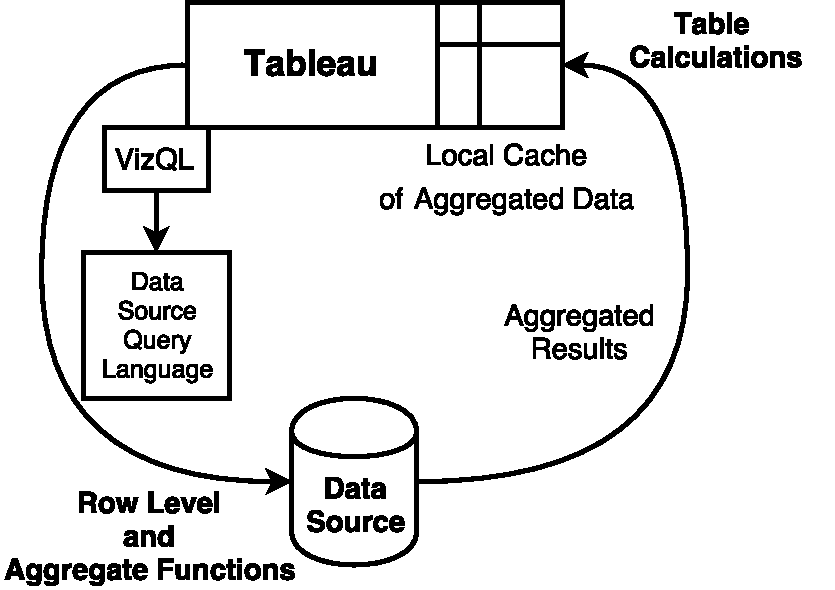
\includegraphics[width=0.8\linewidth]{Figures/TableCalculation}
    \end{center}
    \caption{Execution flow of a table calculation.}
    \label{fig:TableCalculation}
\end{figure}

Tableau gives the user the possibility to use a great variety of operations and allows for writing a custom table calculation, such as:

\begin{itemize}
    \item Computing the running total.
    \item Computing time variance in both absolute values and percentage.
    \item Computing the moving and percentile average.
    \item Ranking or sorting according to specific functions.
\end{itemize}

\subsubsection{Analysis}

Another innovative feature available in Tableau is the possibility to make statistical analyses through built-in mathematical models  or algorithms written in \textbf{R, Python or MatLab} \cite{LearningTableau}. The main built-in models usable in Tableau are:

\begin{itemize}
    \item \textbf{Trend lines}: each trend line added to a chart represents a regression, which Tableau builds according to linear, logarithmic, exponential or polynomial models.
    \item \textbf{Forecasting}: in case of the visualisation of a time series, it's possible to use the \textit{exponential smoothing} method to compute future values according to an exponential function, weighing current value and past values' average; Tableau can also recognize periodic patterns in time series.
    \item \textbf{Clustering}: Tableau uses K-Means algorithm to classify the data on the chosen variables and gives the user the possibility to change the value of K, that is the number of total clusters.
\end{itemize}

\section{Tableau Server}

\textbf{Tableau Server} is a server application used to contain data and metadata of sources and shared workbooks. Through an Access Control List based on accounts, Tableau server allows users to view, interact, download, share and edit a worksheet without the need to install Tableau Desktop. Additionally, through the sharing of an already present data source, a user can create new worksheets without installing the correspondent drivers.

\subsection{Tableau Embedded}

Tableau Server offers the possibility to embed worksheets in a web application using Tableau JavaScript API, which allows for:

\begin{itemize}
    \item Viewing and interacting with the shared view.
    \item Loading and resizing the view dynamically.
    \item Download the view as a PDF or an image.
\end{itemize}

Corresponding user credentials would be required to view the shared charts and plots, but it's possible to use Tableau's \textit{Trusted Authentication} to authenticate the server hosting the application in order to allow all the web app users access to it.
\chapter{Security}

Dal momento che i dati che trattiamo e ricaviamo dall'analisi hanno rilevanza conoscitiva e valore in termini di mercato e ricerca, risulta fondamentale considerare un ambiente sicuro in cui accogliere tali informazioni. Tale perimetro deve però garantire, contemporaneamente alla discrezione relativamente all'accesso del dato, un livello sufficiente di astrazione dalla generica interazione esterna, permettendo un massimo controllo sull'interezza del sistema.

\begin{figure}
	\centering
	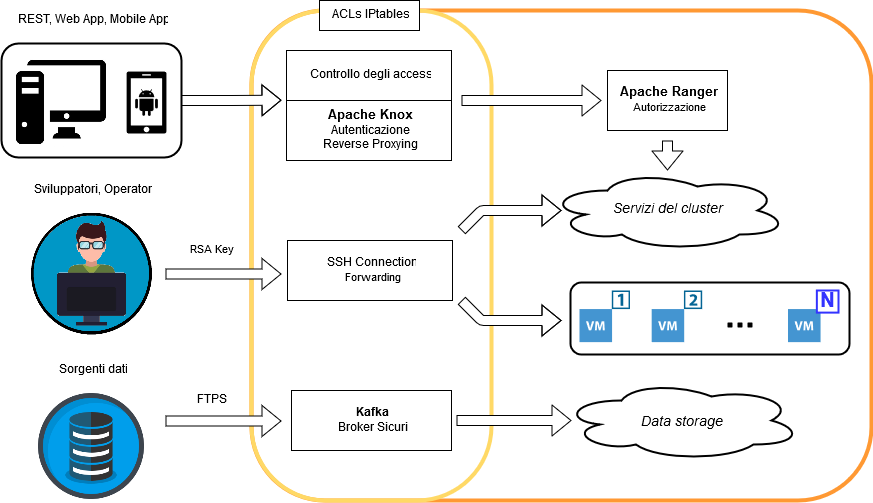
\includegraphics[scale=0.4]{Figures/security_diagram.png}
	\decoRule
	\caption[Infrastructural Stack]{Struttura del perimetro di sicurezza}
	\label{fig:security_diagram}
\end{figure}
La struttura progettata risulta, dunque, articolata su due livelli:
\begin{itemize}
	\item frontend, che si occupa dell'interazione dell'utente con i servizi forniti dal cluster;
	\item cluster, ossia i nodi sottostanti, che garantiscono un livello di sicurezza più specifico per ogni servizio interpellato.
\end{itemize}
Il primo problema da porsi nello sviluppo di una struttura di sicurezza risulta essere la definizione delle entità che possono interagire con il sistema e in quale misura tali interazioni avvengono, in modo da fornire una soluzione adatta sia in termini di confidenzialità per le parti che per facilità d'uso.
\newline
Parliamo, quindi, di:
\begin{itemize}
	\item operatori tecnici: sviluppatori o amministratori del sistema, che necessitano di accessi più profondi e possono lavorare all'interno della rete aziendale.
	\item utenti esterni: clienti o personale generico, che necessitano di utilizzare i servizi del cluster, senza possibilità di modificarne la struttura.
	\item sorgenti dati: data streams esterni, inviano dati su cui si lavorerà con gli strumenti presenti nel cluster.
\end{itemize}
Per ciascun utente si sono considerati approcci differenti, commisurati alle esigenze. 
Le richieste avvengono su un ristretto numero di porte abilitate alla comunicazione con l'esterno e viaggiano su canali sicuri, tramite l'utilizzo di protocolli quali HTTPS, SSH e FTPS.
\newline
In un secondo momento le chiamate vengono autenticate tramite provider dedicati come LDAP o Kerberos, per poi essere sottoposte ad un controllo di autorizzazione, atto a verificare che la richiesta sia congrua ai diritti dell'utente.
\newline
L'esito di ciascun passaggio viene registrato da un servizio di auditing, che permette di tenere traccia delle richieste e degli accessi al sistema, in modo da identificare eventuali abusi o tentativi di forzatura del sistema.

\pagebreak

\section{Knox}

Apache Knox è un Application Gateway, componente della suite di strumenti Hadoop, che fornisce varie funzionalità in termini di sicurezza per clusters Hadoop, specialmente se coadiuvato da altri elementi.
\newline
Nella struttura in esame riveste il ruolo fondamentale di "Reverse Proxying" dei servizi offerti dal cluster e di autenticazione e "Access Control".
\subsection{Reverse Proxying}
Il gateway Knox fornisce un servizio di mascheramento che permette di definire un URL da mostrare all'utente esterno corrispondente a ciascuna chiamata rivolta al cluster. In questo modo è possibile distinguere interfaccia e implementazione del servizio, mantenendo confidenziale la struttura dell'architettura sottostante e garantendo la modularità del sistema.
\newline
Ogni servizio che necessiti di Knox deve essere dichiarato all'interno di uno specifico file di topologia. La topologia è un file XML che dichiara le componenti associate a Knox, quali provider di autenticazione e autorizzazione, e i servizi gestiti dal file in esame.
A questo vengono accompagnati due file di definizione del servizio:
\begin{itemize}
	\item service.xml, che definisce la struttura della chiamata che verrà associata al servizio interessato;
	\item rewrite.xml, che definisce tramite regex la politica di riscrittura che deve essere seguita, prima che la chiamata venga inoltrata al cluster.
\end{itemize}
Le chiamate che possono essere fatte tramite Knox seguono i dettami del protocollo REST, riportando indirizzo, topologia e servizio richiesto nell'URL sottoposto.
% procedimento di reverse proxying ???
\pagebreak

\subsection{Autenticazione e Access Control}
Il gateway Knox si presenta come unico access point sicuro per le interazioni con il cluster, che siano esse tramite API REST che attraverso chiamate HTTP/HTTPS. Ogni richiesta viene inoltrata previa sottomissione di credenziali. Queste vengono autenticate da Knox tramite il provider dichiarato dalla topologia selezionata, LDAP o Kerberos.
Successivamente la chiamata autenticata viene sottoposta all'entità specificata per l'autorizzazione che garantisce controllo sugli accessi ai servizi del sistema.
Infine, una volta garantita la bontà della richiesta, viene sottoposta al servizio per l'esecuzione.
\pagebreak

\section{Ranger}

Apache Ranger \cite{ranger_doc} è un framework che si occupa di definire e gestire la sicurezza del dato all'interno di un cluster Hadoop. Questo avviene tramite l'utilizzo di un sistema di autorizzazione specifico per ogni servizio presente nel cluster che centralizza le logiche di autorizzazione per le varie risorse del sistema. La gestione di Ranger può avvenire sia tramite interfaccia grafica web, sia tramite chiamate REST al nodo su cui risiede il framework. Infine, garantisce una profonda conoscenza per quanto riguarda le interazioni con il cluster, tramite un servizio di audit che osserva le operazioni effettuate in tempo reale e le registra su HDFS o Solr.
\newline

\subsection{Autorizzazione}

Nel momento in cui una richiesta a un servizio del cluster viene autenticata dal provider scelto, deve essere sottoposta al controllo di Ranger, per verificare i privilegi dell'utente nei confronti della risorsa richiesta. È possibile gestire il processo di autorizzazione su due livelli differenti: discriminando rispetto caratteristiche di chi effettua l'accesso o a che unità di lavoro appartiene (access authorization) o relativamente alla risorsa richiesta (resource authorization).
\newline 
All'interno di tali approcci possiamo riconoscere ulteriori distinzioni. Relativamente al controllo degli accessi degli utenti:
\begin{itemize}
	\item Role based (RBAC), che valuta l'accesso in base a criteri di ruolo e privilegi dell'utente;
	\item Attribute based (ABAC), una specializzazione del RBAC, che considera nella valutazione anche attributi aggiuntivi, come indirizzo IP, luogo di login o dati dell'utente.
\end{itemize}
Per quanto riguarda,invece, l'accesso alle risorse, essendo un framework rivolto all'utilizzo in un ambiente Hadoop, Ranger mette a disposizione alcuni plugin per interagire direttamente con i principali servizi presenti nella suite, garantendo un controllo più specifico e profondo riguardo quali operazioni l'utente possa e non possa fare. I plugin sono programmi in Java incapsulati in processi del servizio di riferimento che si occupano di caricare le regole da un server centrale e memorizzarle localmente in un file. Tra i servizi riconosciuti troviamo:
\begin{itemize}
	\item HDFS
	\item HBase
	\item Hive
	\item Yarn
\end{itemize}
Ad esempio, per quanto riguarda Hive, le regole di autorizzazione permettono di specificare per ogni regola quali operatori è possibile utilizzare nelle query al database, chi può effettuarle e a quali campi può avere accesso.
%immagine policy
\newline

\subsection{Regole "Tag Based" e persistenza dei dati}

Versioni più recenti di Ranger hanno introdotto la possibilità di utilizzare regole di sicurezza basate su etichette. Queste vengono attribuite a varie risorse dai vari servizi in modo da definire lo stesso tipo di regola per entità differenti senza doverlo definire esplicitamente, rendendo più semplice le operazioni di controllo degli accessi e di gestione delle risorse. Le etichette e la loro definizione sono tenute in un "Tag Store", mentre un processo di sincronizzazione TagSync si occupa di mantenere le informazioni sempre aggiornate tra i servizi che ne fanno uso.
\newline
Tutte i dati relativi alla logica di sicurezza sono memorizzati in locale, in uno database MySQL su uno degli hosts, che mantiene tutte le informazioni relative a regole e utenti previsti dal framework. La coerenza del sistema viene garntita da un processo di sincronizzazione dedicato che aggiorna le liste di utenti, gruppi e ruoli con LDAP/Active Directory e le opzioni di configurazione con Ambari.
\newline
\chapter{Air Traffic monitoring: a use case}

\section{Introduction}

Air traffic monitoring can be considered a practical use case for the infrastructure described in the previous chapters, being characterised by the Big Data 3 Vs, as there are more than 5000 aircrafts flying any time (\textbf{Volume}), each one of which is transmitting data via transponder signals once every few seconds (\textbf{Velocity}) and, for each data source, data formats can be wildly different from one another, while, additionally, raw data transmitted by aircrafts can be used in conjunction with other kinds of data, such as weather and social networks, for deeper analytics (\textbf{Variety}).

\section{Infrastructure overview}

The infrastructure bones have been built with a series of Virtual Machines provisioned in the \textbf{Azure Pack Cloud-On-Premise} environment provided by the \textbf{VarGroup Data Center} located in Empoli (FI). There are, in total, seven VMs mounting CentOS 7 with the following specifications:
\\    
\begin{table}[!htb]
    \centering
    \begin{tabular}{|c|c|c|c|c|}
        \hline
        \# of VMs & CPUs & Memory & Storage & Hosts \\ \hline
        1 & 1 & 512 MB & 40 GB & \texttt{frontend} \\ \hline
        2 & 4 & 12 GB & 80 GB & \texttt{master-1}, \texttt{master-2} \\ \hline
        4 & 4 & 6 GB & 100 GB & \texttt{slave-1}, \texttt{slave-2}, \texttt{slave-3}, \texttt{slave-4} \\ \hline  
    \end{tabular}
\end{table}

All of these VMs are part of an \textbf{Hortonworks} cluster featuring HDP 2.6.1, deployed via Ambari Blueprint interface through an aptly made scripting suite to automate machine preparation. As additional software used, other than Hortonworks Hadoop distribution, which includes HDFS, YARN, Spark 2, Hive, Kafka, Zookeeper, Ranger, Knox and NiFi, \textbf{Flink 1.4} binaries have been compiled from sources targeting Hortonworks hadoop version and installed for usage on top of YARN, while a Cassandra cluster has been installed on the four slave nodes.

The cluster has been made secure by the gatekeeping provided by Knox and the fact that access is only possible through the front-end machine and only via passwordless SSH by operators and developers. The front-end additionally implements iptables as firewall to prevent access to unwanted ports from external requests.

\textbf{Note:} 10 additional VMs have been provisioned in the same environment for a MongoDB cluster, used as an additional data sink after Flink processing. Two additional distinct Windows Server 2012 machines have been provisioned to host the domain controller for the cluster and Tableau Server.

\section{Deployment \& Operations}

As mentioned, the virtualised cluster has been provisioned in a \href{https://www.microsoft.com/it-it/cloud-platform/windows-azure-pack}{Azure Pack Cloud-On-Premise} environment, which allows to automate the virtual machines' creation and management through \textbf{Azure Powershell} tools and its set of \textbf{cmdlets}\footnote{A \textit{cmdlet} is a lightweight command that is used in the Windows PowerShell environment within the context of automation scripts that are provided at the command line, executing an action and returning a Microsoft .NET Framework object to the next command in the pipeline.} to create, remove and, in general, manage Virtual Machines and their allocated resources.

\subsection{Hadoop Cluster Deployment}
After the virtualised cluster creation, Hadoop and other cluster services need to be installed. In order to do that, as a way to streamline a cluster installation, \href{https://hortonworks.com/products/data-platforms/hdp/}{\textbf{Hortonworks HDP 2.6.1} Hadoop distribution} has been chosen (with Hadoop 2.7.3, from Hortonworks repositories), rather than installing all of the Hadoop services one-by-one. When it comes to the cluster installation, HDP main feature is \textbf{Apache Ambari}\footnote{\href{https://ambari.apache.org/}{Apache Ambari} is a software for provisioning, managing, and monitoring Apache Hadoop clusters, providing an intuitive, easy-to-use Hadoop management web UI backed by its RESTful APIs.} and its Blueprint REST interface for a cluster installation which can be made through a single REST call. For this very reason, a script suite called \textbf{hw-install}\footnote{\href{https://github.com/fedexist/hw-install}{hw-install} is Python 2.7 script suite to automate an Hortonworks cluster installation} has been developed to take advantage of this functionality and automate the cluster preparation and configuration, before the actual deployment.

\textbf{hw-install} is composed of two main packages: \texttt{hw\_install} and \texttt{\justify{hw\_add\_new\_host}}, while the first one handles the installation of an entire cluster given a proper configuration in YAML format, the second one handles the preparation of a new host to be added to an existing cluster via the Ambari Server UI.

Both packages use the same core components for the preparation of cluster hosts:

\begin{itemize}
    \item Set-up of \textbf{passwordless SSH} communication between hosts with a common RSA key identifying the user executing \texttt{hw\_install}, by default and as recommended by Hortonworks Setup guide the user is \textbf{root};
    \item Increasing of the number of \textbf{file descriptors} available in the system;
    \item Installation of the \textbf{NTP} (Network Time Protocol) service, for hosts time synchronization;
    \item Disabling of \textbf{firewall and SELinux}, in order to allow hosts to communicate freely between each other;
    \item Set-up of \textbf{hostnames, FQDNs}\footnote{Fully Qualified Domain Name} \textbf{and DNSs};
    \item Installation on the selected host of the \textbf{Ambari Server}, together with the Ambari Agents, on all of the hosts
\end{itemize}

In addition, \texttt{hw\_install} uses \textbf{Ambari Blueprint} interface, for the cluster deployment, passing the configuration file containing the needed services and their per-component configuration, if any (in absence of this per-component configuration, Ambari will apply default values), and then making a REST call to the Ambari Server which will take care of the installation of the needed components on the selected hosts.

\pagebreak
An example of a configuration file is:
\\

\begin{minted}[breaklines, breakafter="ambari/"]{YAML}
cluster-name: cluster_name
blueprint-name: blueprint_name
ambari-repo: http://public-repo-1.hortonworks.com/ambari/centos7/2.x/updates/2.5.1.0/ambari.repo
Blueprints: # HDP version to be installed
    stack_name: HDP
    stack_version: 2.6
ambari-server: # Host where Ambari Server will be installed
    IP: 192.168.1.1
    FQDN: master.localdomain
hosts: # Other hosts in the cluster
    - IP: 192.168.1.2
      FQDN: slave.localdomain
host-groups:
    - name: master
    hosts: # Hosts belonging to the 'master' host group
        - fqdn: master.localdomain
    components: # Services to be installed in 'master' host group
        - name: YARN_CLIENT
        - name: HDFS_CLIENT
        - name: HIVE_SERVER
        - name: HIVE_METASTORE
        - name: NAMENODE
        - name: ZOOKEEPER_CLIENT
        - name: RESOURCE_MANAGER
        - name: WEBHCAT_SERVER
        - name: ZOOKEEPER_SERVER
        - name: AMBARI_SERVER
.....
\end{minted}
\pagebreak

Once a cluster has been installed, it's easy to add another host to the cluster, using \texttt{hw\_add\_new\_host}: after adding the appropriate \texttt{new-hosts} entries to the configuration file of the cluster, executing this script allows to set-up the host before manually adding it to the cluster from the Ambari Server UI, where it's possible to select the new services to be installed.


\subsection{Flink \& Cassandra Deployment}
For the current use case, it's been chosen to use Flink running on top of YARN, so that there's no need to set up a standalone Flink cluster with its own configuration. In order to use Flink, it's then necessary to download the sources of the needed version, 1.4.0 in this case, and compile it against the Hadoop version which was installed and selecting, if needed, the Scala version which is going to be used while developing the Flink applications.\\
\\
Cassandra deployment is rather straightforward, since, starting from a common \texttt{\justify{cassandra.yaml}} configuration file where all of the nodes have been noted as cluster \texttt{seeds}, it's possible, after importing its repository, to install it directly from CentOS package manager as a system daemon/service.


\subsection{Deployed Software \& Versions}
To sum up, the cluster has been provisioned with HDP 2.6.1, which includes:
\begin{itemize}
    \item Hadoop 2.7.3.2.6.1.0-129 (HDFS, YARN and MapReduce),
    \item Tez 0.7.0,
    \item Hive 1.2.1000, 
    \item ZooKeeper 3.4.6,
    \item Kafka 0.10.1,
    \item Knox 0.12.0,
    \item Ranger 0.7.0,
    \item Spark 2.1.1,
    \item NiFi 1.2.0,
    \item Registry 0.3.0,
    \item Slider 0.92.0.
\end{itemize}

In addition, it's been used Flink 1.4.0 for Scala 2.11 compiled from sources against hadoop 2.7.3.2.6.1.0-129 and Cassandra 3.11.
\\
\\
The cluster is composed of seven machines:
\begin{itemize}
    \item \texttt{frontend}, with Knox and a Nginx reverse proxy installed, used as single point of entry for developers and cluster operators to access cluster services via SSH tunneling. Specifications: 1 core, 512 MB of RAM.
    \item \texttt{master-1}, one of the two master components of the cluster, with an HDFS Namenode, a Zookeeper Server, a Registry MySQL database, a Kafka Broker, Hive Metastore and HiveServer 2 Interactive (support for Hive LLAP daemons), Ranger Admin and UserSync, a NiFi node and Spark2 History Server. Specifications: 4 core, 12 GB of RAM.
    \item \texttt{master-2}, the other master component of the cluster, with the YARN Resource Manager and App Timeline Server, HDFS Secondary Namenode, a Zookeeper Server, a WebHCat Server and HiveServer2 for Hive, a Kafka Broker, a Nifi node, MapReduce2 History Server and Flink binaries. Specifications: 4 core, 12 GB of RAM.
    \item Four slave machines, \texttt{slave-1}, \texttt{slave-2}, \texttt{slave-3}, \texttt{slave-4}, with a YARN Node Manager, HDFS DataNode and Cassandra nodes. Specifications: 4 core, 6 GB of RAM.
\end{itemize}
\pagebreak
\section{Development}

\subsection{Ingestion}

As a primary data source for the use case of Air traffic monitoring, \href{https://www.satori.com/}{Satori} and its air traffic channel have been chosen given the easy to use APIs made available to connect to the data stream. Satori is a portal where organizations can publish their open data and offers a wide variety of channels, that is data endpoints, to be used: from transportation channels, to weather related channels. The \href{https://www.satori.com/channels/air-traffic}{air-traffic channel} republishes data from \href{https://planefinder.net/}{Planefinder}, filtering only aircrafts above 37000 feet of altitude, effectively cutting most of national flights which don't even reach that altitude. In a real world application on air traffic monitoring, it would be necessary to use more than a single data source, additionally using commercial data services such as \href{http://flightaware.com/}{FlightAware} and \href{http://flightradar24.com/}{FlightRadar24} in order to get the most information available.
\\\\
Data Ingestion's pipeline is composed of 2 main components: NiFi and Kafka. Nifi, handles the distributed execution of the script used to connect to Satori and publishes the data to Kafka, which, in turn, handles the queueing and the serving to consumer applications (which is, in this case, a Flink Job).

JSON records ingested from Satori contain the following fields:

\begin{itemize}
    \item \textbf{origin}: IATA code of the airport from which the airplane has taken off.
    \item \textbf{destination}: IATA code of the airport to which the airplane will arrive.
    \item \textbf{aircraft}: model of the aircraft which has transmitted the current record.
    \item \textbf{flight}: public code representing the airplane route.
    \item \textbf{registration}: unique ICAAO identification for the aircraft which has transmitted the current record.
    \item \textbf{callsign}: radar-only code representing the airplane route.
    \item \textbf{lat}: latitude.
    \item \textbf{lon}: longitude.
    \item \textbf{speed}: speed in Knots from the current record.
    \item \textbf{altitude}: altitude in feet from the current record.
    \item \textbf{course}: vector direction in degrees, measured clockwise from north (0°).
    \item \textbf{time}: timestamp since UNIX epoch in seconds of the current record.
\end{itemize}

The ingestion pipeline in NiFi uses in total 4 Processors, as shown in \ref{fig:nifipipeline}. The first Processor is \textbf{ExecuteProcess} and it is used to execute a Python script that connects to Satori through their already mentioned APIs and prints all of the fetched records as lines containing JSON Arrays, on the standard output. The flow continues, then, in the \textbf{SplitText} and \textbf{SplitJson} processors which, respectively, deal with singling out each JSON Array and then extracting each JSON Object, which is the actual record, for it to be published on Kafka via the proper \textbf{PublishKafkaRecord\_0\_10} processor.

\begin{figure}[ph]
    \centering
    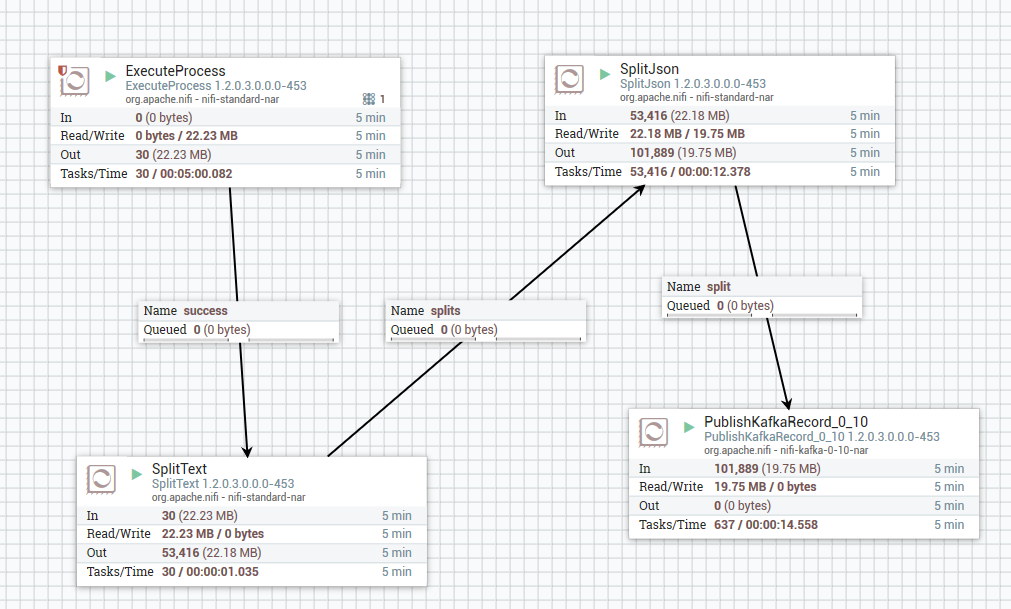
\includegraphics[width=0.7\linewidth]{Figures/nifipipeline}
    \caption{NiFi pipeline used for the ingestion from Satori}
    \label{fig:nifipipeline}
\end{figure}
\pagebreak
In order to get into more details, let's list the entire pipeline:

\begin{enumerate}
    \item \textbf{ExecuteProcess} Processor, where the data fetching actually happens, it runs continuously the following script:
    \\
    \begin{code}
        \begin{minted}{Python}
with make_client(endpoint=endpoint, appkey=appkey) as client:
    class SubscriptionObserver(object):
        def on_subscription_data(self, data):
            for in_message in data['messages']:
                if all(len(str(x)) > 0 for x in in_message.values()):
                    fetched_data.append(json.dumps(in_message))
            got_message_event.set()
    subscription_observer = SubscriptionObserver()
    client.subscribe(
            "air-traffic",
            SubscriptionMode.SIMPLE,
            subscription_observer)
    while got_message_event.wait(10):
        if len(fetched_data) != 0:
            print(fetched_data)
        \end{minted}
    \end{code}
which basically uses Satori APIs to create a client subscribing to the Air Traffic JSON stream, fetching batches of JSON records, filtering out those with empty values and printing each batch on standard output as a JSON array. ExecuteProcess will then create a \textbf{FlowFile} containing as a payload many JSON arrays from subsequent script calls, which will be the input for the following Processor.

\item \textbf{SplitText} simply deals with splitting a single FlowFile, with many JSON arrays, into that many FlowFiles containing only a single JSON array.
\item \textbf{SplitJson}, instead, deals with extracting all of the JSON Objects from the input JSON arrays, generating a FlowFile for each one of them.
\item \textbf{PublishKafkaRecord\_0\_10} is the NiFi Processor which publishes the incoming FlowFiles to a Kafka topic. Its required configuration needs the usual Kafka Producer settings: the broker list, a comma separated list of the broker listeners, in this case \texttt{master-1.localdomain:9092,master-2.localdomain:9092}, the topic in which each record needs to be published, \texttt{air\_traffic}, and the security protocol used to publish, \texttt{PLAINTEXT}. Other than these settings, this Processor needs two components: a \textbf{Record Reader}, needed to deserialize the incoming FlowFiles, and a \textbf{Record Writer}, used to serialize each record before publishing it on Kafka. Said components are services provided by an \textbf{HortonworksSchemaRegistry}, a registry used to store Avro schemas\footnote{\textbf{\href{https://avro.apache.org/}{Avro}} is a data serialization system allowing to define types and possible values for JSON encoded records.} against which incoming records are validated to make sure they follow the specified schema. If validation succeeds, the record is then correctly published on the \texttt{air\_traffic} topic, serialized following the validated Avro schema.
\end{enumerate}

Data ingestion continues, then, in Kafka. As previously mentioned, a single topic called \texttt{air\_traffic} is used, configured with a retention time of 24 hours, a single partition, since throughput is approximately of $20000$ records per minute, accounting to 4 MB per minute, being a relatively sparse stream, and two replicas handled by both the active Kafka brokers.
\pagebreak

\subsection{Processing}

The main backbone of this use case is provided by Flink. After the data is being acquired from NiFi into Kafka, it's processed by a Flink application which then will persist enriched data on HDFS, MongoDB and Cassandra.
\\
Before talking about the Flink application per se, it's worth saying that Flink has been deployed on top of YARN with a Job Manager with 1GB of memory allocated and a single Task Manager with 3GB of memory and 3 slots for parallelism, for a total of 4GB and 4 vCPUs allocated on YARN. 

The Flink application has been written in Scala, making use of the appropriate Scala API provided by Flink. The job has been configured to checkpoint every minute, through an externalised checkpoint, to use as a state backend HDFS and use \texttt{EventTime} as the Stream Time Characteristic.

\subsubsection{Application}

\begin{figure}[h]
    \centering
    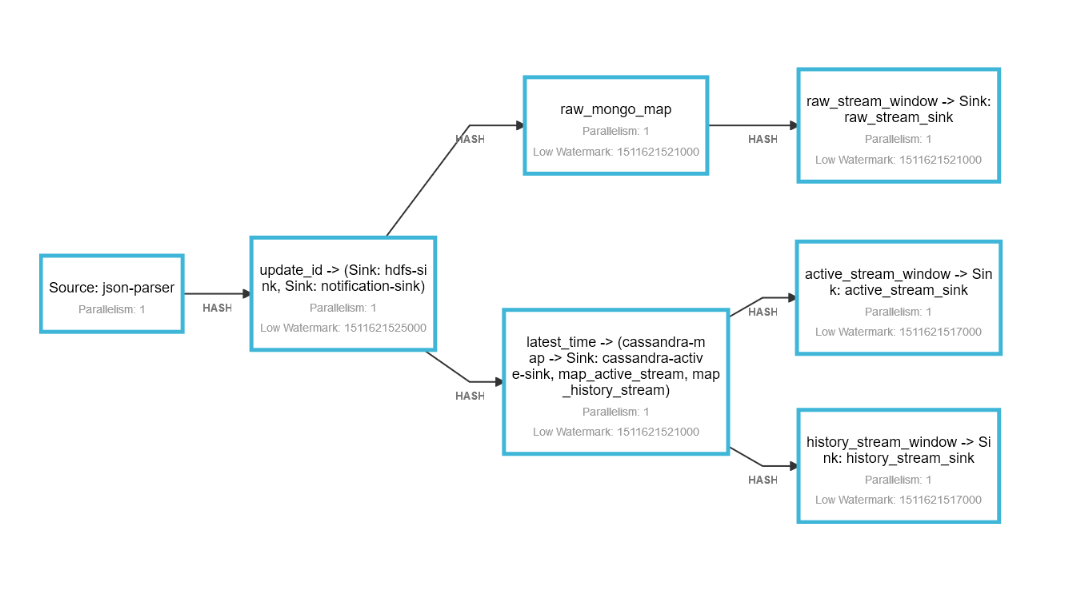
\includegraphics[width=0.8\linewidth]{Figures/flink_job}
    \caption{An overview of the complete DAG of the Flink application described in this section}
    \label{fig:flinkjob}
\end{figure}


\paragraph{Source}
The Flink application has a single source, a Kafka Consumer configured to consume from the \texttt{air\_traffic} topic connecting to both the active kafka brokers on \texttt{master-1} and \texttt{master-2}. Flink's built-in Kafka Consumer must be configured with a deserialization schema, which, in this case, parses from each JSON an \texttt{AirTrafficEvent} using Scala library \href{https://www.playframework.com/documentation/2.6.x/ScalaJson#The-Play-JSON-library}{Play-JSON}.
\\
\begin{code}
   \begin{minted}[breaklines]{Scala}
class JSONDeserializationSchema extends AbstractDeserializationSchema[AirTrafficEvent] {
       
    @throws[IOException]
    override def deserialize(message: Array[Byte]): AirTrafficEvent = {
       
    val obj = Json.parse(message)
    obj.as[AirTrafficEvent]
    }
       
    override def isEndOfStream(nextElement: AirTrafficEvent) = false
}
   \end{minted}
\end{code}

\texttt{AirTrafficEvent} is defined as a Scala case class with three fields wrapping all of the information contained in the original JSON: \texttt{FlightInfo}, containing flight, callsign, registration, origin, destination and aircraft, \texttt{InstantValues}, containing time, altitude, speed and course, and \texttt{Coordinates}, containing latitude and longitude.
\\
\begin{code}
    \begin{minted}[breaklines]{Scala}
//AirTrafficEvent definition
case class AirTrafficEvent
    (flightInfo: FlightInfo,
     coordinates: Coordinates,
     instantValues: InstantValues) extends Event(flightInfo, coordinates, instantValues) with Comparable[AirTrafficEvent]

//FlightInfo definition
case class FlightInfo
    (origin: String,
     destination: String,
     flight: String,
     aircraft: String,
     registration: String,
     callsign: String) extends Serializable

//InstantValues definition
case class InstantValues(speed: Int, altitude: Int, course: Int, time: Date) extends Serializable with Comparable[InstantValues]

//Coordinates definition
case class Coordinates(lat : Double, lon: Double) extends Serializable
    \end{minted}
\end{code}

Since Flink is using EventTime as Time Characteristic of the stream, a timestamp and a watermark should be assigned to every record, in order to be correctly managed for in order consuming and windows. The assigned timestamp and watermark are directly extracted using the \texttt{instantValues.time} field from the parsed \texttt{AirTrafficEvent}, via a \justify{\texttt{BoundedOutOfOrdernessTimestampExtractor}} to make sure that late events within 10 seconds are still correctly processed by Flink.

\paragraph{Operations}

Two main operations are performed on the data flowing through the DAG representing the application: the UID generation of the flight record currently processed and the event processing to get aircrafts which supposedly have arrived to destination.

UID generation is made through \texttt{UpdateIdFunction}, a stateful \texttt{ProcessFunction} processing each element of the stream according to the following pseudo-code:

\begin{minted}{Python}
if is_active_flight(element):
    id = old_id # mantained as state
else:
    id = id + 1
    notify_on_new_flight()
event = event_with_id(element, id)

return event
\end{minted}

It takes as input a \texttt{KeyedStream} of \texttt{AirTrafficEvent}s and outputs an \texttt{AirTrafficEventWithId} stream: the ID is an integer counter which gets increased each time a new instance of a flight is being detected and used to create the actual id of the outputted objects concatenating the flight id with this integer ID (e.g. the first instance of flight \texttt{AZ775} will have id \texttt{AZ775-1}). 

\begin{code}
    \begin{minted}{Scala}
    val streamWithId : DataStream[AirTrafficEventWithId]= stream
        .keyBy(_.flightInfo.flight)
        .process(new UpdateIdFunction())
    \end{minted}
\captionof{listing}{A KeyedStream of AirTrafficEvent processed into an AirTrafficEventWithId stream}
\end{code}
\pagebreak
The function handling the detection of a new instance of a flight is based off an heuristic strategy using the latest available information about the position, speed and time of the flight. This is needed because the stream may be inaccurate when it comes to transoceanic flights, passing over dead zones, without any radar at range being able to catch their transponder signals. The heuristic is described by the following Scala snippet:
\\
\begin{minted}[breaklines]{Scala}
val activeUpperBound = Time.minutes(5) // 5 minutes
val notActiveLowerBound = Time.hours(5) // 5 hours
val threshold = Time.minutes(120) // 60 minutes
val (last_lat,last_lon) = lastKnownPosition.value match {
    case null => return false
    case _ => lastKnownPosition.value
}
val last_speed = lastSpeed.value  match {
    case 0 => return false
    case _ => lastSpeed.value
}
val last_time = lastTime.value  match {
    case 0 => return false
    case _ => lastTime.value
}

if(new_time - last_time < activeUpperBound.toMilliseconds) true
else if(new_time - last_time > notActiveLowerBound.toMilliseconds) false
else
    Math.abs(distFrom(new_position, (last_lat, last_lon))/knotsToMetersSeconds(last_speed)
        - (new_time - last_time)/1000) < threshold.toMilliseconds/1000

\end{minted}

in which can be seen that there are three main conditions being checked:
\begin{enumerate}
    \item if the difference between the timestamps is less than a certain upper bound (default 5 minutes), meaning that we received an event from the current flight recently and implying the it is active.
    \item if the difference between the timestamps is greater than a certain lower bound (default 5 hours), meaning that we haven't received an event from the current flight in a while, implying it's a new instance of a flight. This case is used as a discriminant for flights flying over dead zones.
    \item provides a prediction based off the estimated time to reach the latest position from the previous last known position, at constant speed=last\_speed, and the actual time taken to reach the latest position.
\end{enumerate}

This way, we are able to be reasonably certain that an aircraft, even after passing over a dead zone for more than 5 minutes, is still flying towards its destination and we are not dealing with another instance of the same flight. A more accurate heuristic would be possible with a data source not cutting under 37000 feet and using an additional data source with the airports and their position, integrated within the stream structure.

Additionally, whenever a new instance of a flight is detected a side-output is used to forward outside of the \texttt{ProcessFunction} an \texttt{Alert} containing the relevant event, together with the event type, which is, in this case, \texttt{newAirplane}.
\\ \\
Just like it has been mentioned, the second operation executed on the stream concerns the event processing used to detect aircrafts arriving to their destination. Since it's been noted that the data stream is incomplete, in order to demonstrate \textbf{FlinkCEP} capabilities when it comes to event processing, instead of using a pattern that detects variations in altitude and speed to correctly determine the sequence of events implied by an aircraft approaching to an airport, it's been used a simple pattern based on the timing out of events sequences.

\pagebreak

The pattern is implemented as follows:
\\
\begin{minted}{Scala}
val airplaneArrivalPattern = 
Pattern
    .begin[AirTrafficEventWithId]("flying")
        .where(_.airTrafficEvent.instantValues.altitude >= 37000)
        .oneOrMore
    .notNext("disappearing")
        .where(_.airTrafficEvent.instantValues.altitude >= 37000)
        .within(Time.minutes(30))

// Associate KeyedStream with pattern to be detected
val patternStream  = CEP.pattern(streamById, airplaneArrivalPattern)
//Side output where timed out events are forwarded
val outputTag : OutputTag[Alert] = OutputTag[Alert]("side-output")
// How to handle timed out and in-time events
val result: DataStream[AirTrafficEventWithId] = 
    patternStream.select(outputTag) { //Timed out events
        (pattern: Map[String, Iterable[AirTrafficEventWithId]], 
        timestamp: Long) => {
            val alert = new Alert(pattern("flying").last, 
            AlertType.disappearedAirplane.id) alert
        }
    } { //In time events
        (pattern: Map[String, Iterable[AirTrafficEventWithId]]) =>
            pattern("flying").last}   
// Collect timed out events from the main stream
val alertStream = result.getSideOutput(outputTag)
alertStream.addSink(new NotificationSink()).uid("notification-sink")
    .name("notification-sink")
\end{minted}

and is basically structured on the analysis of a Keyed Stream, keying on the event id, such that if there's no event within 30 minutes from the last one, the pattern times out, an \texttt{Alert} is created, from the last event stored, and then forwarded to the notifications' sink.

\paragraph{Sinks}

The Flink application has three main sinks where data is forwarded to be stored after processing: \textbf{MongoDB}, \textbf{Hive via HDFS} and \textbf{Cassandra}. On these three sinks there are three types of data stores: a \textit{raw} data store where all the records are saved after being enriched with their unique ID, an \textit{history} data store where it is saved a single record per flight, updated as needed, and an \textit{active} data store used for live monitoring purposes. An additional sink is used for the \texttt{Alert}s constructed during the stream processing.

\textbf{MongoDB} is used as sink for all of the three data stores, with adequately defined collections, while \textbf{Cassandra} is used for the \textit{active} data store, and \textbf{Hive} via HDFS is used only for the \textit{raw} and \textit{history} ones.

\pagebreak

Cassandra Sink in Flink is added through the \texttt{CassandraSinkBuilder} used to specify the query to be used while inserting the records in the table:
\\
\begin{minted}{Scala}
// Add sink to Cassandra cluster
CassandraSink.addSink(
    airtrafficEvents
        .map(_.toCassandraTuple)
        .javaStream)
.setQuery(
    s"""UPDATE air_traffic.active
    |SET lat = ?, lon = ?, speed = ?,
    |    altitude = ?, course = ?, flight = ?,
    |    origin = ?, destination = ?, aircraft = ?, time = ?
    |    WHERE id = ?;""".stripMargin)
.setClusterBuilder( new ClusterBuilder {
def buildCluster(builder: Cluster.Builder): Cluster = {   
    builder.addContactPoint("slave-1")
    builder.addContactPoint("slave-2")
    builder.addContactPoint("slave-3")
    builder.addContactPoint("slave-4")
    builder.build()
}
}).build()
\end{minted}

\pagebreak

On Cassandra's cluster, composed as already mentioned previously, by the four slave nodes, has been specified an \texttt{air\_traffic} keyspace, configured with a replication factor of 3 via the replication strategy \texttt{SimpleStrategy}. Within this keyspace the following table has been defined:
\\
\begin{minted}{SQL}
CREATE TABLE air_traffic.active (
    id text PRIMARY KEY,
    altitude int,
    course int,
    destination text,
    flight text,
    aircraft text,
    lat double,
    lon double,
    origin text,
    speed int,
    time timestamp
) WITH default_time_to_live = 600
       AND gc_grace_seconds = 3600
\end{minted}

in order to contain all of the active aircrafts currently flying. All of the default configurations have been maintained, except for the TTL of the records which has been configured to 10 minutes and the interval of the garbage collection of the table tombstones (expired records after the TTL) which has been set to 1 hour, instead of 1 day.
\\ \\
Notifications sinks are rather simple \texttt{SinkFunction}s which take as input the \texttt{Alert} and make an async \texttt{POST} request, through a \href{https://dispatchhttp.org/Dispatch.html}{Dispatch} asynchronous HTTP client, to the local notification server, implemented using Firebase FCM, about which we'll talk about later on.

\pagebreak
Hive is not the direct destination of the Flink sink. As a matter of fact, an HDFS sink is used to write all of the records in JSON format, partitioned in folders according to their timestamp. As a result, each event will be bucketed in the appropriate folder and this folder will be considered as a partition of an Hive external table configured using the \textbf{JsonSerDe} to read all of the files.
\\
\begin{minted}{Scala}
val hdfsSink = new BucketingSink[AirTrafficEventWithId](hdfs_path)
hdfsSink.setBucketer(new EventDateTimeBucketer("YYYY-MM-dd"))
hdfsSink.setBatchSize(1024 * 1024 * 64) // 64MB files size

streamWithId.addSink(hdfsSink).uid("hdfs-sink").name("hdfs-sink")
\end{minted}

while the Hive external table is defined as it follows:
\\
\begin{minted}[breaklines]{SQL}
CREATE EXTERNAL TABLE IF NOT EXISTS json_dump
( `origin` string,`flight` string,
`course` int,`aircraft` string,
`callsign` string,`registration` string,
`lat` double,`lon` double,
`altitude` int,`speed` int,
`destination` string,`time` timestamp,
`_id` string)
PARTITIONED BY (`dt` string)
ROW FORMAT SERDE 'org.apache.hive.hcatalog.data.JsonSerDe'
WITH SERDEPROPERTIES ('timestamp.formats'='YYYY-MM-dd HH:mm:ss.SSS')
STORED AS TEXTFILE
LOCATION '/flink/air_traffic/json_dump';
\end{minted}

Starting from this very table, which maintains records in text format, uncompressed, further optimizations will be performed before the final storage within Hive.

\subsubsection{Post-processing: HDFS to Hive}

As we already determined, Hive is not the direct target of Flink, since we're using an Hive external table to read all of the Json files written by the HDFS sink. Using a textfile format is not optimal for storage purposes, since it's not a compressed format and we'd like to save as much storage as possible. For this reason an additional table, in the appropriate database in Hive, has been defined to be the final target of the raw stream written in HDFS. Additionally, from this table, another table called history is filled, aggregating all of the records of a flight in a single record with arrival date and departure date.

To sum up, there are three tables stored in Hive:
\begin{itemize}
    \item \texttt{json\_dump}, external table reading the Json files written by Flink;
    \item \texttt{raw} in \texttt{air\_traffic} database, containing an optimized version, for storage and query purposes, of \texttt{json\_dump} 
    \item \texttt{history} in \texttt{air\_traffic} database, aggregating \texttt{raw} creating a single record for each flight.
\end{itemize}

The raw table is defined to use ORC as storage format, to use Hive partitioning on the date and to be clustered in 100 buckets, in order to make sure that, if needed, a query concerning a certain subset of flights wouldn't read all of the files composing the table.
\\
\begin{minted}[breaklines]{SQL}
CREATE TABLE IF NOT EXISTS air_traffic.raw(
`origin` string,`flight` string,
`course` int,`aircraft` string,
`callsign` string,`registration` string,
`lat` double,`lon` double,`altitude` int,`speed` int,
`destination` string,`time` timestamp,`_id` string)
PARTITIONED BY (`dt` string)
CLUSTERED BY (flight) INTO 100 BUCKETS
STORED AS ORC;
\end{minted}

\pagebreak

The history table is instead defined with the additional fields \texttt{arrival\_date} and \texttt{departure\_date}, removing all of the instant values, deemed as not needed, as it follows:
\\
\begin{minted}{SQL}
CREATE TABLE `history`(
`_id` string, 
`date_depart` timestamp,`date_arrival` timestamp, 
`flight` string,`callsign` string, 
`registration` string,`aircraft` string, 
`origin` string,`destination` string)
PARTITIONED BY (`dt` string)
\end{minted}

Both these tables are filled in a periodic batch operation, scheduled every 20 minutes, through \texttt{INSERT OVERWRITE} queries on the current partition (date): whereas the \texttt{raw} is a simple overwrite from \texttt{json\_dump} as they have the same schema,  \texttt{history} aggregates the time field via \texttt{MAX()} and \texttt{MIN()} Hive aggregated functions as shown below:
\\
\begin{minted}{SQL}
INSERT OVERWRITE TABLE air_traffic.history PARTITION(dt="${PARTITION}")
(SELECT
    `_id`,
    MIN(time) AS date_depart,
    MAX(time) AS date_arrival,
    flight,callsign,
    registration,aircraft,
    origin,destination
FROM air_traffic.raw
WHERE dt="${PARTITION}"
GROUP BY 
    `_id`,flight,callsign,
    registration,aircraft,
    origin,destination)
\end{minted}

Periodic scheduling has been set using \texttt{crontab} functionalities of CentOS, which is used to execute a Python script called \texttt{hive\_loader} which executes the needed queries. \texttt{Hive\_loader} has four flags used to determine which queries has to be executed:
\begin{enumerate}
    \item \texttt{bootstrap}, which creates all of the tables used.
    \item \texttt{update}, which controls the scheduled execution for the update of raw and history tables.
    \item \texttt{add\_partition\_update}, used after midnight to definitively update \texttt{raw} and \texttt{history} of the previous day, while adding a new partition to \texttt{json\_dump}.
    \item \texttt{drop\_partition}, used to drop the previous day partition, before deleting it.
\end{enumerate}

Together with the aforementioned tables, additional tables have been created and filled to be available to Tableau for visualisation purposes:

\begin{itemize}
    \item \texttt{aircrafts}, containing the ID model and its capacity in terms of number of passengers.
    \item \texttt{airports}, containing, for each airport, its complete name, its IATA code, its continent and its ISO country and region codes.
\end{itemize}
\pagebreak

\subsection{Serving \& Security}
Our infrastructure's security is handled on several layers by a variety of services striving to offer access on data and visualisations to the users and to let the developers maintain and upgrade the system while providing extensive security on the data and protection from unauthorised access.

\begin{figure}[h]
	\centering
	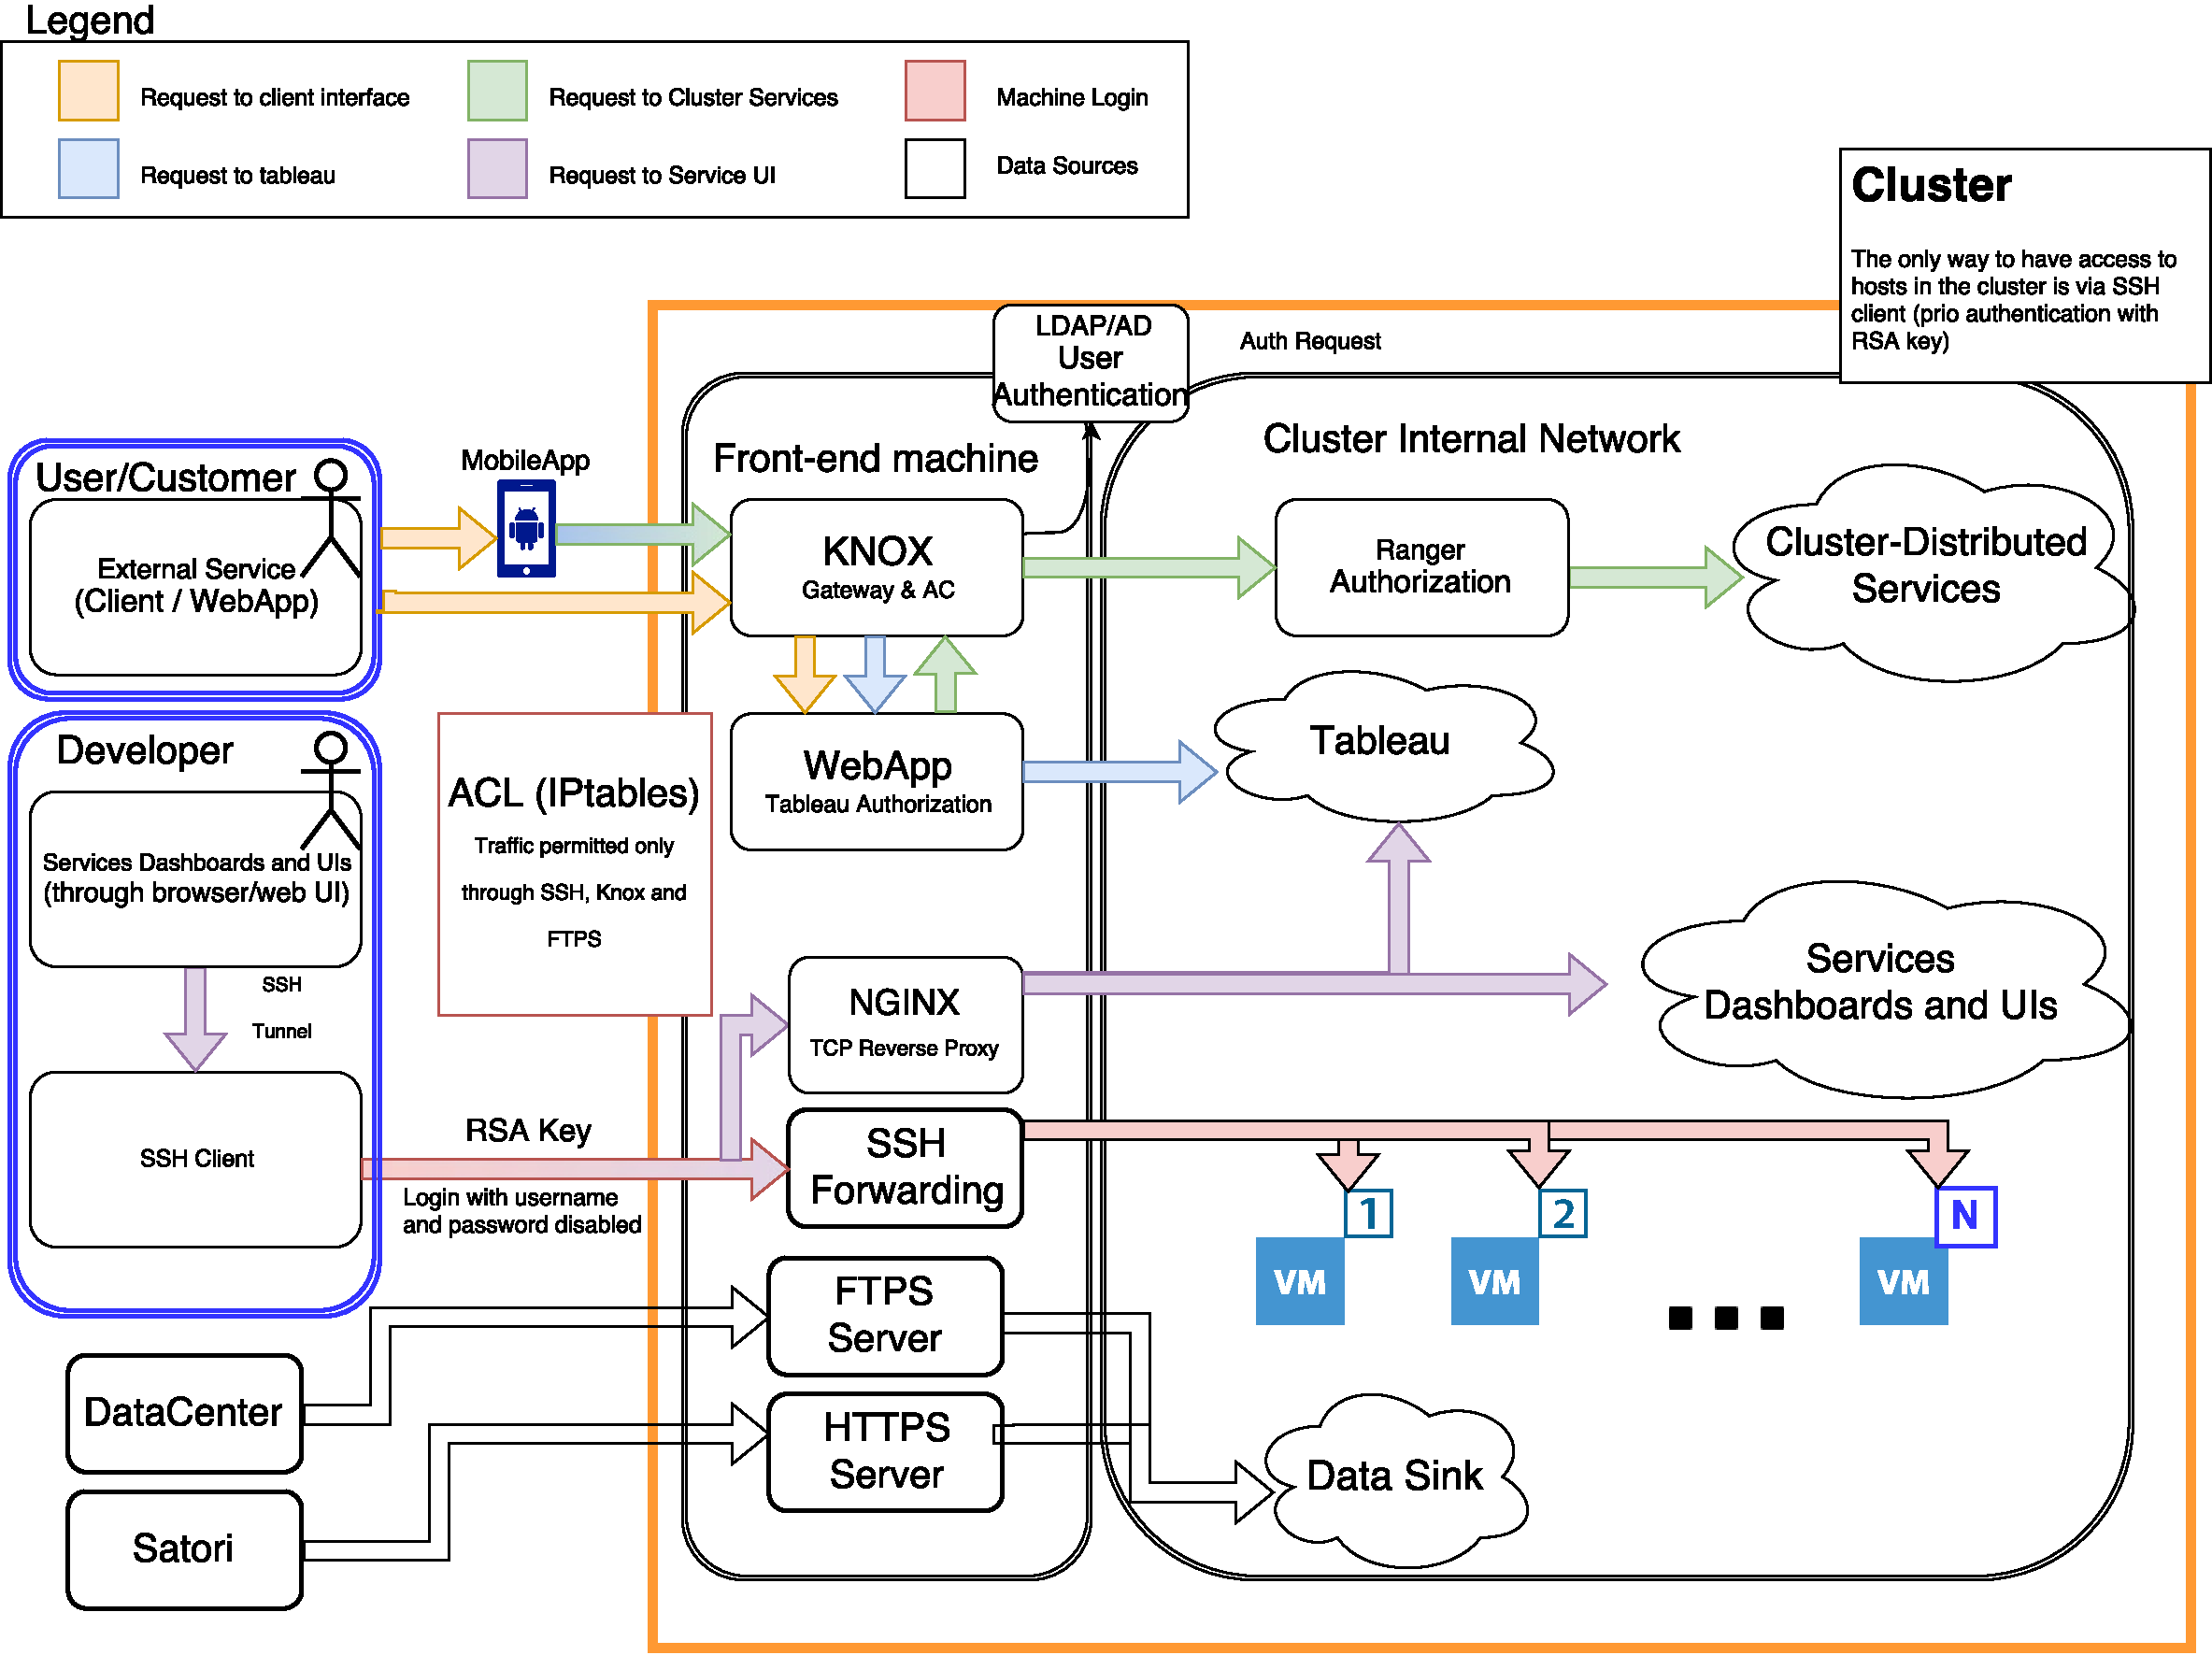
\includegraphics[scale=0.3]{Figures/SecurityStructureDiagram}
	\decoRule
	\caption[Security Structure Diagram]{A diagram to represent our Security Structure}
	\label{fig:SecurityStructureDiagram}
\end{figure}

We have structured the Security and Serving architecture through two main abstractions: the \textbf{cluster} and the \textbf{flows}.
\subsubsection{Cluster}
The \textbf{cluster} is our whole Big Data Infrastructure comprised of several nodes which for our purposes are divided as such:
\begin{itemize}
	\item One (or two in High Availability) Domain Controller, which handles user creation, update and authentication.
	\item One (or two in High Availability) Front End node, which manages access to the cluster's services and data.
	\item Several Inner Cluster nodes, the machines on which visualising, processing and storing is actually done.
\end{itemize}

\paragraph{Domain Controller}
The Domain Controller is not accessible from outside the cluster and can communicate freely with the Front End and the Inner Cluster Nodes.\\
It hosts \textbf{Active Directory}, a directory service by Microsoft comprised of several components for domain and security management such as LDAP, Kerberos, and DNS.\\ \\
As a directory service, the Active Directory instance consists of a database containing an hierarchy of objects, objects are a very high abstraction that can represent a variety of things, but for our purposes can either be Users or Groups; Groups contain one or more Users and Users may be part of one or more Groups. \\Users are identified by a username and a strong password, thus the Domain Controller can authenticate an Agent thanks to this information. \\
Through LDAP, authorised Users can access and modify Objects in the Active Directory. Each authentication, whether failed or successful is logged.\\ \\
We have defined two groups: \texttt{cluster\_users} and \texttt{cluster\_operators}, the meaning of which is further specified down the line by each layer of protection.

\paragraph{Front End}
The Front End node is the only machine accessible from outside the cluster and can communicate with the Domain Controller and the Inner Cluster nodes. \\
Access to the Front End from outside is possible through a selected number of ports and only with secure protocols (HTTPS, FTPS and SSH), this is obtained with the use of ACLs, implemented on CentOS through iptables. The Front End features Apache Knox and Nginx to route requests to the right services and stores RSA private keys of all the Inner Cluster nodes plus a public one for each developer's own private key, so that passwordless SSH connections can be established from developers' machines to Front End and from Front End to Inner Cluster nodes. \\
\\
Nginx is a HTTP and HTTPS reverse proxy that also supports TCP reverse proxying and can be used to route whatever HTTP request or TCP connection from the Front End machine to the proper Inner Cluster node's service. \\
\\
Apache Knox also serves as a reverse proxy, this time specifically for Hadoop cluster's services requiring authentication and authorisation. Its topology is implemented so that an authorised Active Directory user called Knox.domain, through LDAP, can ask for authentication on an incoming request's sender and access to lists of Users and Groups.\\ If the user is authenticated, Knox can then grant access to the request, thanks to the information on Users and Groups, to the target service and route it accordingly or deny it. \\ Outcoming requests are bundled with the authenticated username, so that inside the Inner Cluster nodes other services can use that information securely. Requests at this stage are logged whether denied or accepted, along the name of the alleged requester in order to be investigated in case of failures or attempted breaches.\\ \\
The topology is set so that all our custom services for access to MongoDB and Hive are available to all users belonging to the cluster\_users or cluster\_operators group, while the standard Hadoop services are available only to those in the latter.
\\
\\
The Front End machine also hosts programs for data ingestion, an FTPS server and a NodeJS application that serves the WebApp.

\paragraph{Inner Cluster Nodes}

All the other nodes in the Cluster are considered Inner nodes as they are barred from outside and can only communicate with the Domain Controller and the Front End. \\
These machines hold all processing services, databases and visualisation tools plus the interfaces to access their resources. Here, requests incoming from the Front End have been already authenticated and given access, but each service can enact additional policies on those, to add a layer of security and to protect from mistakes (i.e. DROP DATABASE). \\ \\
While each service might manage its own policies, most Hadoop applications delegate this burden to Apache Ranger: Ranger, thanks to its Usersync agent synchronises its list of Users and Groups with the Active Directory's one, so that further authorisation policies can be defined on the same cluster\_users and cluster\_operators seen before. \\ \\
 Thus we have decided to give users in cluster\_users clearance for the use of SELECT on our Air-Traffic database, while deletions are forbidden to them; on the other end, users in cluster\_operators are also able to update and delete records.
\\ At this level, requests are logged again, to log failed authorisations and to assign actions' responsibilities to the appropriate users.

\subsubsection{Flow}
We define the flow, in the context of the security of our system, as the path requests and responses travel from a class of external Actors to the cluster and back.
\\ \\
In general, the flow starts from an Actor outside the cluster sending a request (i.e. A User through a MobileApp), the request is received by the Front End Node, accepted or denied; accepted requests are then forwarded and routed to the target Inner Node's service which handles the request and generates a response accordingly, the response is then set back following the same path backwards to the Actor.
\\ \\
We have distinguished three different flows, each pertaining to a different Actor:
\paragraph{User}
A user, which is a person or agent requesting access to our stored data, can query our databases and view visualisations built upon stored data service through a WebApp or a Mobile App.\\
Queries are sent to our custom REST APIs to Knox on the Front End machine; the user, who must be present in Active Directory and be part of cluster\_users, is authenticated and authorised to proceed with its request, this request now routed to the Inner Cluster is received by our REST servers, parsed into queries and sent to the appropriate database with the user's credentials, the query is received by MongoDB security or Apache Ranger for Hive, whatever the recipient, its policies are enforced on the request; the result of the query is then sent back to the REST server which encapsulate it and send it back as a response to the user.
\\ \\
Visualisations are requested to the WebApp from outside the cluster, the WebApp requires a login for authentication and then authorises the user following its own policies, as a Tableau user or operator, the WebApp then requests tokens to be consumed watching visualisations on behalf of the user and then responds with a HTML page embedding the visualisations and tokens. This method prevents the need of having to authenticate the same users multiple times.
\paragraph{Developer}
While able to access the cluster as clients, the developers can also connect to the Front End through an SSH client provided they have the Front End private key, as username and password are disabled, while connected they can further their connections to all nodes to access the local file system. What's more, through tunnelling, several TCP connections can be forwarded through the SSH connection from the developer localhost to the Front End machine; there Nginx routes Front End local connections to several clusters' machines, providing a safe passage from the developer's machine to the required Dashboard or User Interface.
\paragraph{Data Source}
Lastly Data Sources must be able to send data to our secured clusters to be stored on the databases, in order to do that two options are available: an application on the Front End can pull data constantly on an endpoint (for example through HTTPS) or the providers can push data on a server on the Front End (for example through FTPS), then another application is responsible to transfer newly acquired data from the Front End to the Inner Cluster Nodes
\pagebreak

\subsection{Accessory Services}

While not strictly related to Big Data, the results we archive and process may be used for several different endeavours; we wanted to offer additional features for presentation, other than Visualisations, in the form of push notifications for mobile devices and REST APIs to access securely data in our databases.

\subsubsection{Push Notifications}
We have decided to send Push Notifications whenever a plane departs and is directed towards one of our airports of interest or whenever a plane is approaching its destination, descending below 37000 feet of altitude.
\\
To offer this service we have implemented a solution based on one of the many components of the Google Mobile Platform: \textbf{Firebase Cloud Messaging}.

\paragraph{Firebase Cloud Messaging}

Firebase Cloud Messaging (FCM) is a service for mobile and browser push notifications offered through a REST API listening on Google Firebase servers; the requests sent to this API are formatted in JSON specifying information on the message sent and on the receivers.
What's more, the Firebase Server assigns to each device attached to our application a unique and expiring token to identify what devices will be receiving each notification.
\\
In more detail, FCM supports two different ways to send messages.

\begin{itemize}
	\item \textbf{Token based messaging}: The request for the notification includes a list of the tokens assigned to the recipient devices. 
	\item \textbf{Topic based messaging}: The devices are required to subscribe to topics, requests are sent specifying the topic of which the notification is part of, so that subscribers can receive it.
\end{itemize}  

Seen that our topic in this case would have been airports, whose list is giant and ever growing, we have concluded that topic based messaging would be highly impractical and therefore chosen to use the token based solution and to handle the routing of notifications through a filtering application.

\paragraph{Local Server}
To handle users' data, filtering of notifications and the construction of requests to be forwarded to Firebase, we have implemented a middleware server using \textbf{NodeJS}, called \textit{Notifire}, listening on internal nodes, which offers a REST API customised for our needs.
\\
The server manages users' data, keeping a table on Hive representing the connection between Device Unique ID, Notifire Token and a list of airports the user is subscribed to. Changes to this table can be issued by the users through a request to the server, it is mandatory for the mobile application to send an update after obtaining a new token from Firebase, so that the table is always up to date.
The table is also cached in memory for performance reasons.
\\ \\
As mentioned, the server offers a REST service to ingest notifications and forward it to Firebase. In more detail, the server expects a JSON containing information on a departing plane such as: airport of origin, airport of destination, type of aircraft, flight number and other spatial or temporal values.
\\ \\
For each received and accepted JSON, the server writes a list of tokens that are subscribed to the airport of destination and creates a message informing of the departure. It then creates a request with those data and send it to the Firebase server which in turn sends the actual notification to all target devices and responds back to our server with a report of the action.
\pagebreak
\subsubsection{REST APIs}
As for REST APIs we have implemented two servers written in Python with the use of \textbf{Flask} library: \textit{Arnia}, offering a simple REST interface to write queries in SQL, and \textit{KhanUI}, a similarly easy to use REST API to query MongoDB through the use of PyMongo's own syntax.

\paragraph{Arnia}

Arnia accepts calls to its address in this form from within the cluster (Knox handles calls from outside in HTTPS converting them to the proper inner call and managing authentication of <user>): 

\begin{code}
	\begin{minted}[breaklines]{Bash}
http://<host.inner.ip>:<arnia_port>/query?query=<query>&user.name=<user>
	\end{minted}
\end{code}

To make this template a more comprehensible example:

\begin{code}
	\begin{minted}[breaklines, breakafter=&]{Bash}
http://10.0.0.24:8888/query?query=SELECT+*+FROM+history_aggregated+limit+1&user.name=dummy_user
	\end{minted}
\end{code}

The server would then respond with a JSON object representing the table output by the query; in particular for this example, provided dummy\_user has the required privileges to be allowed by Ranger, Arnia would return a list of records showing two flights, like this:
\\
\begin{code}
	\begin{minted}{javascript}
{Output: [{history_aggregated._id: TP1510-1, 
        history_aggregated.aircraft: A320, 
        history_aggregated.callsign: TAP1510, 
        history_aggregated.date_arrival: 2017-10-12 04:35:08.0, 
        history_aggregated.date_depart: 2017-10-12 00:46:27.0, 
        history_aggregated.destination: LIS, 
        history_aggregated.dt: 2017-10-12, 
        history_aggregated.flight: TP1510, 
        history_aggregated.origin: ABJ, 
        history_aggregated.registration: CS-TNQ}]}
	\end{minted}
\end{code}

\pagebreak
The server's core part of the code to handle this calls is here presented.
\\
\begin{code}
	\begin{minted}[breaklines]{Python}
@app.route("/query", methods=['GET','POST'])  # routes GET and POST requests made to server_ip/query to the inner code
    def query():
    if request.method == 'POST':  # filters out GET requests
        query = request.args.get("query")                # get query body from args
        username = request.args.get("user.name")        # get username from args (this was authenticated by Knox and can be used for authorisation)

        with pyhs2.connect( # connects to hive 2 interactive, to a specific database, in this case: air_traffic
        	host='10.0.0.50',  # hive 2 ip        
            port=10500, # hive 2 port            
            authMechanism="PLAIN", # without ssl because knox already protects our perimeter
            user=username, # we pass our username to authorisation
            database='air_traffic') as conn:
        
        with conn.cursor() as cur:                
            cur.execute(query)                                # executes query and saves results and metadata, the function itself prevents injection, while ranger prevents unauthorised users to modify the database
            
        output_dict = format(cur)

        return json.dumps({'Output' : output_dict}, sort_keys=True, indent=4, default=json_util.default)    # returns query result
	\end{minted}
\end{code}

\paragraph{KhanUI}

Exactly in the same way as Arnia for Hive, KhanUI accepts queries written to a specific address and returns a JSON with the result from MongoDB, the only difference being in the syntax of the query language.
As the core of the code has been already covered for Hive, we'll just bring another example of call and show its response.

Let's say we want to find the average speed, in knots, for each type of aircraft. Following the PyMongo syntax that would be:

\begin{code}
	\begin{minted}[breaklines, breakafter=&]{Bash}
db.active.aggregate([{$group:{_id:"$aircraft",speed:{"$avg":"$speed"}}}])
	\end{minted}
\end{code}

Which in URL form with some encoding would translate to:

\begin{code}
	\begin{minted}[breaklines, breakafter=speed]{Bash}
http://10.0.0.24:8889/query?query=db.active.aggregate%28%5B%7B%27%24group%27%3A%7B%27_id%27%3A%27%24aircraft%27%2C%27speed%27%3A%7B%27%24avg%27%3A%27%24speed%27%7D%7D%7D%5D%29&user.name=airtraffic
	\end{minted}
\end{code}

And for which the response would be:

\begin{code}
	\begin{minted}{javascript}

{
    Output: [
    {
        _id: E75L, 
        speed: 377.5
    }, 
    {
        _id: BLCF, 
        speed: 440.0
    }, 
    {
        _id: E170, 
        speed: 386.0
    }
    ]
}
	\end{minted}
\end{code}
\pagebreak

\subsection{Visualisation}

With the files processed by Flink and stored on MongoDB, Hive and Cassandra we have built several workbooks on Tableau:

\begin{itemize}
	\item \textbf{Live Map}: A map of the world tracking all active flights in real time (Using either MongoDB or Cassandra as data source).
	\item \textbf{Inbound Flow}: Set of different charts to analyse the flow of flights directed towards an airport of choice (Using either MongoDB or Hive as data source).
	\item \textbf{Outbound Flow}: Set of different charts to analyse the flow of flights departing from an airport of choice (Using either MongoDB or Hive as data source).
	\item \textbf{Flight Route}: A route tracked on the map of the world showing the path followed by an aeroplane of choice (Using MongoDB as data source).
\end{itemize}
\subsubsection{Connection to Data Source}

In order to connect Tableau to a data source two middlewares are required: a \textbf{Connector}, to translate Tableau's own VizQL to the target database query language, and an \textbf{ODBC} in which to specify the address and port in which the database is to be found to do the actual connection.
\\
Tableau uses internally a relational model and VizQL is therefore a query language for such models; while for relational databases, such as Hive, the query translation is pretty straightforward, for NoSQL databases like MongoDB and Cassandra the conversion is done with an additional step in which a schema is produced to translate the Document based and Key/Value models into relational models.

\subsubsection{Live Map}
The live map is used to monitor and track in real time planes flying all over the world. Data for this view are collected from Cassandra's Active table or MongoDB's Active collection through a live connection; this connection allows us to refresh the map as soon as new data are available in the database.
\\
The two most important variables for the construction of such graphic are latitude and longitude, used by Tableau to draw a marker on the map. Such marker, by default, is a bullet point, but in order to add a new dimension to the view we added a custom marker showing a plane directed towards the actual direction the flight is headed to.
\\
As for interactivity from the view, it is possible to read other details of a single plane or to use one or more of several filters:
\begin{itemize}
	\item \textbf{Origin}: Airport whence the plane departed.
	\item \textbf{Destination}: Airport where the plane is headed towards.
	\item \textbf{Flight}: The unique code given to a flight.
	\item \textbf{Aircraft}: The aircraft's model's unique code.
\end{itemize}

Figure \ref{fig:LiveMap} shows a close up of the middle east without any filtering.
\begin{figure}[h]
	\centering
	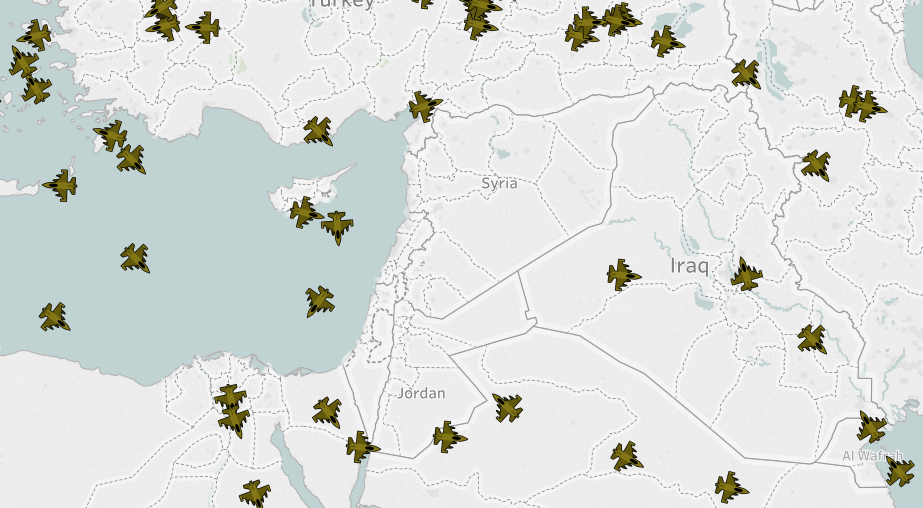
\includegraphics[width=0.9\linewidth]{Figures/LiveMap.png}
	\caption{A close up of the live map over the middle east}
	\label{fig:LiveMap}
\end{figure}

\subsubsection{Inbound Flow}

The second view built aims to present historical data of flights that have landed at an airport. For this kind of periodic analysis for which we have not need of real time connections, we have chosen to use the extract connection; this extract is updated each day and guarantees superior performances in charts' rendering.
\\
Before the extraction, we have set up a join between historical data and collections with information on aircrafts and airports in order to enrich the data source, furthermore fields not utilised in the presentation have been cleansed to lighten the load.
\\
Data are presented in three dashboards focusing on:

\begin{itemize}
	\item \textbf{Flights}: The total number of flights landed at an airport.
	\item \textbf{Aircraft}: The type of aircraft of those flights.
	\item \textbf{Passengers}: The total number of passengers landed at an airport.
\end{itemize}

Whatever the focus, the first useful operation is to filter by selecting an airport for which to analyse the flow. After that several temporal filters are available with complete control of the granularity of time through drill-down and drill-up. It is also possible to change type of chart from classical histogram to geographical maps and heat maps.

Figure \ref{fig:FlightsViz} shows a histogram depicting the flow of flights from the world towards Albuquerque in the month of November from 8 AM to 8 PM, day by day.

\begin{figure}[h]
	\centering
	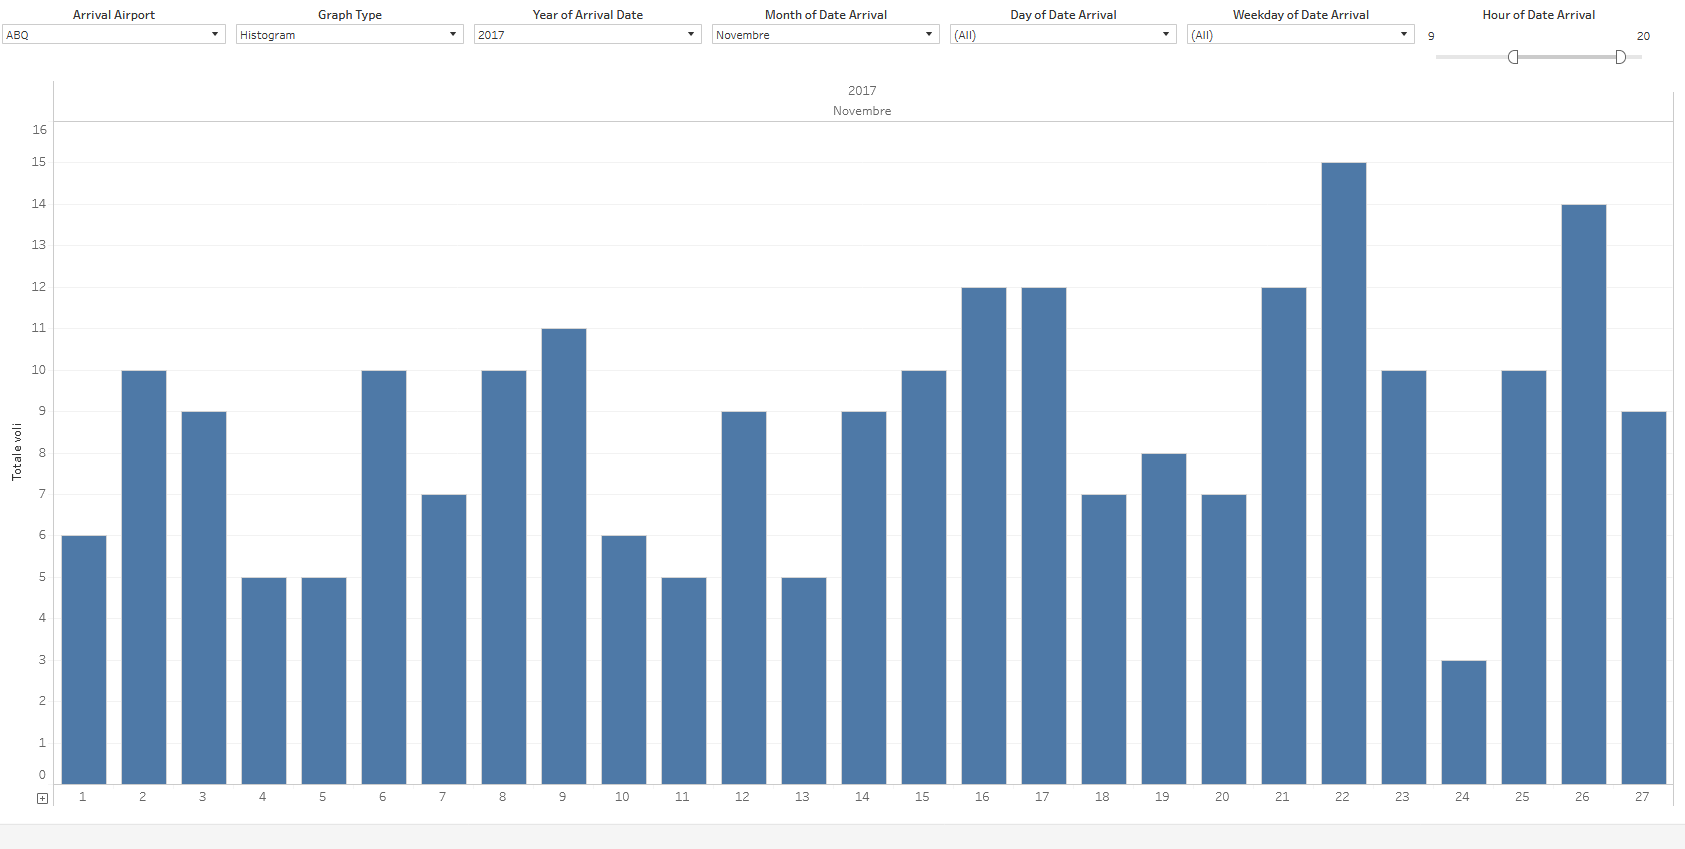
\includegraphics[width=0.9\linewidth]{Figures/FlightsViz.png}
	\caption{Inbound Flow for Albuquerque day by day 8 AM to 8 PM, November}
	\label{fig:FlightsViz}
\end{figure}

\subsubsection{Outbound Flow}
A carbon copy of the inbound flow has been realised to analyse the flow departing from an airport.\\
This duplication is done in order to optimise performances on both views. From an implementation point of view the only change is in the join condition to use during the extract creation and the use of the time of departure as timestamp, instead of the time of arrival.

Figure \ref{fig:PassengersViz} shows a map depicting the main destinations of the passengers departing from Genoa in October and November.

\begin{figure}[h]
	\centering
	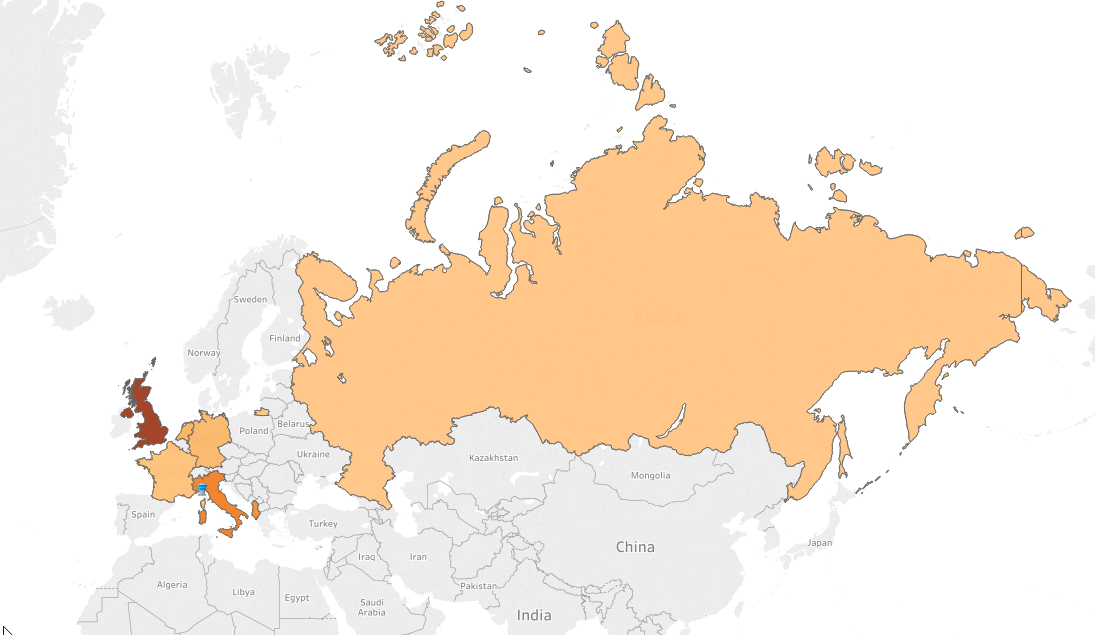
\includegraphics[width=0.9\linewidth]{Figures/PassengersViz.png}
	\caption{Outbound Flow of passengers for Genoa, October and November}
	\label{fig:PassengersViz}
\end{figure}

\subsubsection{Flight Route}
Given a flight code, it is possible to draw the path the aeroplane followed on each day for that route. This view shows the limits of Satori as an end-point, because we can only see messages coming from a height over 37000 feet, cutting the taking off and the landing parts of the fare.

 Figure \ref{fig:RouteViz} shows, through a set of points coming from consequent messages from the same plane, the route of flight UA914, from Paris to Washington, of October 25th; here it can be seen the filter cutting data below 37000 feet in action.
\begin{figure}[h]
	\centering
	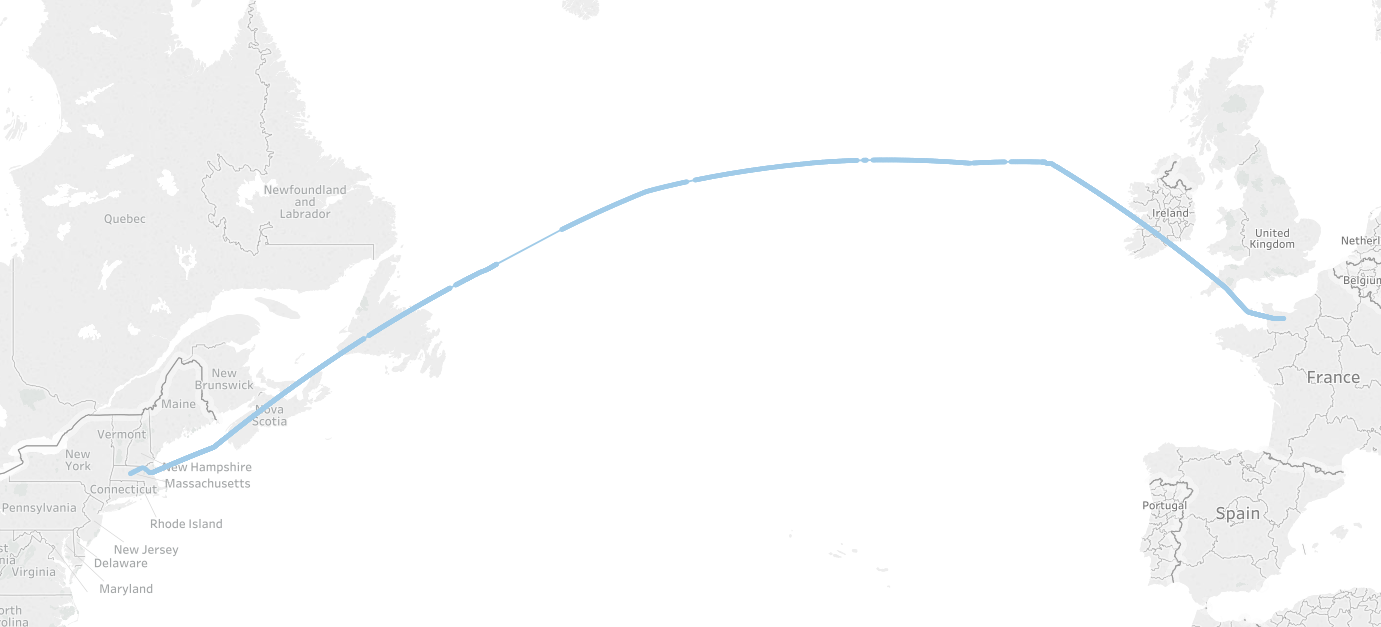
\includegraphics[width=0.9\linewidth]{Figures/RouteViz.png}
	\caption{The route of flight UA914, from Paris to Washington, of October 25th}
	\label{fig:RouteViz}
\end{figure}
This view is built with a live connection with the use of Custom SQL. Thanks to the definition of an ad hoc query, MongoDB's Raw collection is queried using the flight code as a parameter.
The query is then converted to an aggregation pipeline in MongoDB with a dedicated process, resulting in a response within few seconds, in spite of the huge size of the collection (more than a billion documents).
\subsubsection{Publishing on Tableau Server}
Once the workbooks have been created, we proceeded by publishing all the views on Tableau Server. For this purpose, we have defined two user groups with different rights: the Devs who inherit the powers and rights of the Publisher and can create, edit and interact with the workbooks; the Users which inherit the right of the Interactor and can, therefore, only interact with the workbooks.

In order to use the views freely, it had been necessary to save the required credentials for the authentication on the data sources directly on the Tableau workbook.
Finally, we have scheduled a daily update at 4 AM to refresh the extracts for the visualisations of historical data.

%----------------------------------------------------------------------------------------
%	THESIS CONTENT - APPENDICES
%----------------------------------------------------------------------------------------

%\appendix % Cue to tell LaTeX that the following "chapters" are Appendices

% Include the appendices of the thesis as separate files from the Appendices folder
% Uncomment the lines as you write the Appendices

%% Appendix A

\chapter{Frequently Asked Questions} % Main appendix title

\label{AppendixA} % For referencing this appendix elsewhere, use \ref{AppendixA}

\section{How do I change the colors of links?}

The color of links can be changed to your liking using:

{\small\verb!\hypersetup{urlcolor=red}!}, or

{\small\verb!\hypersetup{citecolor=green}!}, or

{\small\verb!\hypersetup{allcolor=blue}!}.

\noindent If you want to completely hide the links, you can use:

{\small\verb!\hypersetup{allcolors=.}!}, or even better: 

{\small\verb!\hypersetup{hidelinks}!}.

\noindent If you want to have obvious links in the PDF but not the printed text, use:

{\small\verb!\hypersetup{colorlinks=false}!}.

%\include{Appendices/AppendixB}
%\include{Appendices/AppendixC}

%----------------------------------------------------------------------------------------
%	BIBLIOGRAPHY
%----------------------------------------------------------------------------------------

\printbibliography[heading=bibintoc]

%----------------------------------------------------------------------------------------

\end{document}  
